\graphicspath{{Chapter5/Chapter5Figs/}}

\chapter{A dynamical network model of mTOR signalling reveals TSC-independent mTORC2 regulation}
\label{chap:A dynamical network model of mTOR signalling reveals TSC-independent mTORC2 regulation}
This chapter describes a systems biology-based investigation of mTORC2 regulation as described in \citep{DallePezze2012a}. The results here focus on the modelling point of view and only include \emph{in vitro} experimental work necessary for model validation and test. All the \emph{in vitro} data included in this project were collected by Annika Sonntag, PhD student supervised by Dr Kathrin Thedieck, Department of Bioinformatics and Molecular Genetics, Freiburg University, Germany. A copy of the published work, which includes the \emph{in vitro} experimental data used for parameterising and testing the model, is attached in Appendix \ref{appendixA}.

\section{Introduction}
\label{paper1-sec:Introduction}
In this project an insulin-mTOR network model integrating both mTORC1 and mTORC2 was built and used to investigate alternative mTORC2 activation mechanisms. In contrast to mTORC1, little is known about mTORC2 upstream regulation (see Section \ref{sec:Upstream signalling pathways of mTOR}). mTORC2 is mainly regulated by growth factors (see Section \ref{subsec:The insulin insulin-like signalling pathway}), but the molecular mechanism has not yet determined. \\
Many substrates of mTORC2 are proteins belonging to the family of AGC kinases (see Sections \ref{subsec:mTOR-dependent regulation of AGC kinases}, \ref{sec:Downstream targets of mTORC2}). Using these AGC kinases as indicators of mTORC2 activity, the TSC1/TSC2 complex has been implicated in mTORC2 activation by insulin. It was found that TSC1/TSC2 inhibition reduces phosphorylation of Akt at S473 \citep{Inoki2005, Huang2008, Huang2009complex, Huang2009signaling}, which contrasted with TSC1/TSC2 inhibition increasing mTORC1 activity \citep{Veelen2011}. Two models have been proposed to explain mTORC2 regulation by TSC1/TSC2, one involving direct mTORC2 activation by TSC1/TSC2 \citep{Huang2008, Huang2009complex, Huang2009signaling}, the other by an indirect mechanism through inhibition of PI3K in response to TSC1/TSC2 ablation via mTORC1-p70-S6K-dependent negative feedback loop (NFL) activation \citep{Yang2006tsc1}. However, data showing that mTORC2 contributes to proliferation in TSC2-null cells suggests that 
mTORC2 can be active in the absence of TSC1/TSC2 \citep{Goncharova2011}. A third hypothesis for mTORC2 activation is through a PI3K-independent mechanism, which has been identified in Dictyostelium \citep{Kamimura2008pip3, Lee2010mTORC2, Charest2010, Cai2010}. Interestingly, in mammals, several cellular processes that are regulated by mTORC2 have been described as PI3K independent \citep{Jacinto2004, Sarbassov2004, Worthen1994, Zheng1997, Kamada2005}.\\
To distinguish among the possible mTORC2 activation mechanisms and to determine whether they acted independently or in combination, a dynamical model was developed, assuming that different modes of mTORC2 regulation would result in distinguishable, dynamical network responses. The model was parameterised with dynamic quantitative time course data and its predictions experimentally validated. Then, perturbations were used to simulate and experimentally test alternative network structures connecting upstream insulin signalling to mTORC2. This approach also provided the benefit of both a structural and dynamical network analysis \citep{Papin2005}.\\
In contrast to the previous hypotheses, TSC1/TSC2 complex was found not to be a direct activator of mTORC2 and that mTORC2 activity was insensitive to the mTORC1-induced NFL. Although PI3K was inhibited by the NFL, activation of the NFL-insensitive mTORC2 also required active PI3K. Therefore, none of the three literature-based hypotheses was confirmed and we proposed a new hypothesis that insulin signalling activated mTORC2 through a PI3K that was insensitive to the NFL. This new model fitted all our collected experimental data.

\section{Results}
\label{paper1-sec:Results}

\subsection{Development of a dynamical insulin-TOR network model}
\label{paper1-subsec:Development of a dynamical insulin-TOR network model}
Initially, a static network model in SBGN format \citep{lenovere2009systems} of insulin-mTOR signalling was established as a means to integrate current knowledge \citep{Zoncu2011, Howell2011, GarciaEcheverria2011, Polak2009, Cybulki2009, Feldman2010, Sengupta2010} and as a platform to chose appropriate targets for measurement (Figure \ref{fig:2002469_supp_fig1}). It is impractical to work with such a large network, due to the high number of parameters and the difficulty in obtaining sufficient experimental data under reasonable time and cost. The extended model presented in Figure \ref{fig:2002469_supp_fig1} was therefore abstracted by selecting (1) regulation mechanisms with an important role in dynamical behaviour (e.g. the activation of mTOR complexes by the presence of both amino acids and insulin, the pathways connecting these stimuli to the mTOR complexes, and the NFL from p70-S6K to IRS), and (2) measurable molecules and interactions distributed across the network (Y1146-phosphorylated IR, the S636-
phosphorylated IRS1, S473- and T308-phosphorylated Akt, S2448- and S2481-phosphorylated mTOR,  T246- and S183-phosphorylated PRAS40, and T389-phosphorylated p70-S6K). These readouts are marked with an asterisk in Figure \ref{fig:2002469_supp_fig1}. This simplified network shows insulin signalling propagating from the IR through the TSC1/TSC2 complex to the mTORC1 complex and includes p70-S6K, PRAS40, and Akt. In addition, mTORC1 induction by amino acids was included. At this stage, no upstream pathway regulating mTORC2 was assumed (see Figure \ref{fig:2002469_fig1}). \\
Studies suggesting that TSC1/TSC2 regulates mTORC2 commonly used Akt phosphorylated at S473 (Akt-pS473) as an mTORC2 readout. However, Akt activity depends on PI3K-dependent relocalisation to the plasma membrane and subsequent phosphorylation at T308 by PDK1 and at S473 by mTORC2 \citep{Pearce2010}. PI3K and Akt are inhibited in the absence of the inhibitory TSC1/TSC2 complex, due to mTORC1 and NFL hyperactivation. Consequently, under conditions of TSC1/TSC2 deficiency and NFL activation, monitoring Akt-pS473 does not distinguish between PI3K, PDK1, and mTORC2 activity, and therefore may not be a suitable readout to investigate the mode of mTORC2 regulation by TSC1/TSC2 \citep{Huang2009complex}. Other AGC kinases that are targeted by mTORC2 (SGK and PKC) have similar issues \citep{Jacinto2008, Bruhn2010}. In this study mTOR-S2481 was used as a direct marker of mTORC2 activity in addition to using Akt-S473. Details about the specificity of mTOR-S2481 as an mTORC2 readout for HeLa cells can be found in \citep{
Copp2009} and in \citep{DallePezze2012a, DallePezze2012b}.

\subsection{Parameterisation of the network model}
\label{paper1-subsec:Parameterisation of the network model}
Immunoblot-based phosphorylation time-courses for network components along the signalling cascade were generated to parameterise the model depicted in Figure \ref{fig:2002469_fig1}. Data were collected from HeLa cells under amino acids/insulin starvation and restimulation conditions and quantified from 1 min up to 2 hours post induction with amino acids/insulin. The model parameters were estimated using the mean time course, computed from four time-course repetitions (Figure \ref{fig:2002469_fig2}). The initial concentrations of the species in their non-phosphorylated state were determined directly from these semi-quantitative data (see Section \ref{paper1-subsec:Modelling}). For all other species, the initial concentrations were set to 0. \\
Due to the known difficulty in calibrating a large number of parameters from the data \citep{Chen2010, Moles2003, Zhan2011}, in this case kinetic rate constants, parameter estimation was divided into calibration phases (see Figure \ref{fig:2002469_supp_fig3}). In Phase 1 of the parameter estimation, isolated modules that could be calibrated independently within the network, were identified. Because the IR regulation was not affected by the rest of the network, the 3 parameters governing the kinetics of IR activation by insulin, dephosphorylation to a refractory state and transition to a receptive state could be isolated and independently calibrated. In Phase 2, due to the lack of knowledge about mTORC2 upstream, a model that was independent of the pathway by which mTORC2 was activated, was generated. The regulation of the mTORC2 substrate Akt-S473 and mTORC2 component mTOR-S2481 were temporarily modelled with two auto-activation mechanisms, which were then calibrated using Akt-pS473 and mTOR-pS2481 
experimental datasets. This guaranteed to reproduce Akt-pS473 activation while maintaining mTORC2 isolated from the network. During Phase 2, a total of 24 reaction rate constants were estimated using eight experimental readouts. Finally, in Phase 3, the autoactivation mechanism of Akt-pS473 was replaced with a phosphorylation mediated by mTORC2-pS2481. Because the initial induction of Akt-pS473 occurred before mTOR-pS2481 was induced (see Figure \ref{fig:2002469_fig2}), mTORC2-pS2481 alone could not completely reproduce the dynamics of the experimental data for Akt-pS473. mTORC2 is not the only PDK2 candidate that may phosphorylate Akt-S473; therefore, an additional PDK2 species was introduced and parameters governing the phosphorylation of Akt-S473 under the influence of the two kinases, were re-estimated. In this phase, three kinetic rate constants were estimated using the Akt-pS473 experimental data. \\
Each of these phases was resolved using an iterative procedure (see Figure \ref{fig:2002469_supp_fig4}). This procedure is summarised by the following steps: 
\begin{enumerate}
 \item The initial values of the parameters that needed optimisation were assigned by random generation;
 \item the calibration was repeated until a set of parameters with consistent values was identified;
 \item this set of parameters was fixed and the remaining free parameters were calibrated again by repeating the process. 
\end{enumerate}
Once this process of parameterisation was complete, the simulated time courses matched the experimental data for all the analysed mTOR network readouts (Figure \ref{fig:2002469_fig2}). The ordinary differential equations (ODEs) and estimated parameters for the general model are provided in Tables \ref{tab:2002469_supp_tab1}-\ref{tab:2002469_supp_tab2}. Identifiability analysis, which indicates whether the parameters can be estimated with confidence from the available data, and sensitivity analyses, which indicates how sensitive model behaviour is to variation in each parameter, for the general model are shown in Figures \ref{fig:2002469_supp_fig5}-\ref{fig:2002469_supp_fig6}. Importantly, the identifiability analysis did not show high correlation between estimated parameters indicating that they could indeed be identified.

\subsection{Validation of the mTORC1 branch}
\label{paper1-subsec:Validation of the mTORC1 branch}
If a parameterised model correctly represents the biological mTOR network dynamics in response to amino acids/insulin, model simulations must accurately reflect the dynamics of known network responses to a gradual perturbation. To validate the mTORC1 branch of the model, the network was perturbed by gradually inhibiting mTORC1 first \emph{in silico}, and then experimentally by Raptor knock down (shRaptor). The model was used to simulate the effect of gradual mTORC1 inhibition on the activation dynamics of the direct mTORC1 substrate p70-S6K-pT389, at several time points after induction with amino acids/insulin. \\
The model predicted a constant increase in p70-S6K-pT389 signal from 10 min to 2 hours after induction. Furthermore, the model also predicted that p70-S6K-pT389 would decrease starting 10 minutes after induction in a near linear manner in response to gradual Raptor (mTORC1) inhibition, whereas there should be no detectable increase or Raptor-dependent change in p70-S6K-pT389 below 5 min after induction (see Figure \ref{fig:2002469_fig3}A). This simulated quantitative p70-S6K-pT389 response upon gradual mTORC1 inhibition (see Figure \ref{fig:2002469_fig3}B) was experimentally validated (see Figure \ref{fig:2002469_fig3}, C and D) at 3, 20 and 45 min, also indicated in the simulation in Figure \ref{fig:2002469_fig3}A by the green lines. The simulations (Figure \ref{fig:2002469_fig3}B) and the experimental results (Figure \ref{fig:2002469_fig3}D) monitoring p70-S6K-pT389 activity in response to gradual Raptor inhibition at 20 and 45 min after induction with amino acids/insulin consistently showed an overall 
increase in signal at 45 min and no signal at 3 min after induction. \\
Therefore, the model accurately reproduced the dynamic behaviour of the mTORC1 substrate p70-S6K-T389 upon gradual mTORC1 inhibition.

\subsection{Alternative models of mTORC2 regulation by TSC1\fshyp{}TSC2}
\label{paper1-subsec:Alternative models of mTORC2 regulation by TSC1/TSC2}
Two alternative mechanisms of TSC1/TSC2-dependent regulation of mTORC2 have been suggested: either direct activation or indirectly through mTORC1 and NFL \citep{Huang2008, Huang2009signaling, Yang2006tsc1}. Since the different suggested molecular mechanisms by which TSC1/TSC2 regulates mTORC2 should result in mechanism-specific changes in the dynamics of the mTORC2 readouts, the response of the readouts to network perturbations should be predictable and distinguishable through dynamical modelling. \\
On the basis of the existing literature, we postulated three different hypotheses for the molecular connection, or lack thereof, between TSC1/TSC2 and mTORC2 (see Figure \ref{fig:2002469_fig4B}): 
\begin{description}
 \item[Hypothesis 1 (TSC-dependent):] TSC1/TSC2 directly activates mTORC2 in response to insulin, and has opposite effects on mTORC1 and mTORC2
 \item[Hypothesis 2 (NFL-dependent):] mTORC2 is activated by insulin through PI3K, but independently of Akt and TSC1/TSC2, however mTORC2 activity can be inhibited indirectly by TSC1/TSC2 ablation through NFL-mediated inhibition of PI3K;
 \item[Hypothesis 3 (PI3K-independent):] mTORC2 is activated by insulin in a manner that is independent of both TSC1/TSC2 and PI3K.
\end{description}
These hypotheses were directly implemented into the established model, re-using the same kinetic parameters. To keep the hypotheses as comparable as possible, each hypothesis shared the network topology of this general model but assumed a specific mTORC2 upstream regulator according to each hypothesis (see Figure \ref{fig:2002469_fig4B}). These kinetic parameters regulating mTORC2 were re-estimated according to each hypothesis (see Tables \ref{tab:2002469_supp_tab1}, \ref{tab:2002469_supp_tab3}). The total goodness-of-fit for the general model and each hypothesis showed that no model could be statistically rejected (see Table \ref{tab:2002469_supp_tab4}), in accordance with the following: 

\begin{lemma}
\label{lemma:model derivation}
Let $\mathcal{M}$ be a model correctly parameterised with some data\footnote{This assumes that the model parameters are structurally and practically identifiable (see Section \ref{subsec:Identifiability analysis}).} and $s$ a species in $\mathcal{M}$. If a modifier $f$ directly upstream of $s$ is selected and re-calibration solely of the dynamics of $s$ maintains a close fit between the simulated time course for $s$ and the experimental data for $s$, then all the time course curves downstream of $s$ will continue to fit their corresponding data. 
\end{lemma}
\begin{proof}
Let $U$ be the set of the upstream species of $f$ ($U = \{ upstream\_species(f) \}$) and $D$ be the set of the downstream species of $d$ ($D = \{ downstream\_species(s) \}$) by applying a cut of the feedback loops. Depending on the existence of a feedback loop connecting an arbitrary species $d \in D$ to an arbitrary species $u \in U$, there exist two cases.\\
Case 1: $\nexists \; d \rightarrow u \;|\; d \in D, u \in U$. After model re-calibration, the time-course of $f$ remains unchanged and the time-course of $s$ is not affected by the dynamics of the network. Since the simulated time course of $s$ still fits the experimental data for $s$ by hypothesis, the signalling cascade from $s$ does not significantly differ, maintaining the fitting of the species in $D$ with their corresponding experimental data.\\
Case 2: $\exists \; d \rightarrow u \;|\; d \in D, u \in U$. In this case, the time-course of $f$ is also modulated by some $d \in D$ and $s$ dynamics are therefore affected by the network. However, $f$ can be interpreted as downstream target of $s$ beyond the application of the cut. Thus, for the previous case, the simulated time course of $f$ maintains the fit with its corresponding experimental data.
\end{proof}

For each hypothesis, time course simulations and experimental validation for the mTORC2 readouts mTOR-pS2481 and Akt-pS473, the PI3K readout Akt-pT308, and the mTORC1 substrate p70-S6K-pT389 (see Figure \ref{fig:2002469_fig4C}) were performed. The curves for all other analysed network components are provided in Figure \ref{fig:2002469_supp_fig7}. The simulations matched the experimental time courses, indicating that the hypotheses were compatible with the observed dynamics for mTORC2 activation and more generally for the mTOR signalling network. Further experimental validation of these models for the mTORC1 branch, monitoring p70-S6K-pT389 can be found in \citep[Fig. 7A]{DallePezze2012a}. Identifiability and sensitivity analyses for the three models representing each hypothesis are shown in Figures \ref{fig:2002469_supp_fig8}-\ref{fig:2002469_supp_fig13}. 


\subsection{Perturbations of alternative models of mTORC2 regulation}
\label{paper1-subsec:Perturbations of alternative models of mTORC2 regulation}
As independent parameter estimation for the three models could not clearly reject any of the previous hypotheses, gradual network perturbations of TSC1/TSC2, the NFL (through perturbation of mTORC1), or PI3K were computationally applied and then experimentally tested. The idea was that the hypotheses might have been rejected by first perturbing the respective upstream modulators of mTORC2 as determined for each hypotheses for each model and then finding experimental inconsistencies with the predicted perturbations. In formal terms:
\begin{definition}
\label{definition:experimentally correct connection}
Let $t : f \rightarrow s \;|\; f, s \in Species$ be a connection. Then, $t$ is said \emph{correct} if it can be experimentally proved. $t$ is said \emph{incorrect} if it can be experimentally negated. 
\end{definition}

\begin{lemma}
\label{lemma:model perturbation}
Let us assume the conditions established in Lemma \ref{lemma:model derivation} and that all the connections besides the connection $t : f \rightarrow s$ for a model $\mathcal{M}$ correctly parameterised with some data, are \emph{experimentally correct}. 
If the introduced upstream connection $t$ is \emph{correct} then the model output following perturbation of $f$ will \emph{necessarily} maintain a fit with the corresponding data. Instead, if $t$ is \emph{incorrect}, then the model output following perturbation of $f$ will not \emph{necessarily} maintain a fit with the corresponding data.
\end{lemma}
\begin{proof}
This lemma shows a semi-decidability property for model rejection. \\
Case 1: $t$ is \emph{correct}. Then, a simulated perturbation of $f$ is consistent with the corresponding data upon experimental perturbation of $f$, since the model was correctly parameterised. \\
Case 2: $t$ is \emph{incorrect}. Then, a simulated perturbation of $f$ may or may not be consistent with the corresponding data upon experimental perturbation of $f$. In fact, if this is not consistent, then the network can be clearly rejected. Instead, if the prediction is still consistent, then nothing can be asserted with such a simulated perturbation and further testing is required. Instances of this case can arise due to model abstraction or multiple input besides $f$ to $s$.
\end{proof}
From Lemma \ref{lemma:model perturbation}, a tool for rejecting a model was formalised in case of detection of model inconsistency with some data upon perturbation.\\

In this study, the connection $t$ referred to as the link from a kinase regulating mTORC2 and mTORC2 itself. For each of the three perturbations and each of the three hypotheses, the dynamical network response of the readouts of mTORC2-pS2481 activity (see Figure \ref{fig:2002469_fig5A}), Akt-pS473 activity (see Figure \ref{fig:2002469_fig5B}), Akt-pT308 activity (see Figure \ref{fig:2002469_supp_fig14}), and p70-S6K-pT389 activity (see Figure \ref{fig:2002469_supp_fig15}) were detected. These simulated perturbations unambiguously distinguished network behaviour, indicating specific experimental testing treatments, and highlighted time points in which these differences occurred (see green lines in Figures \ref{fig:2002469_fig5A}-\ref{fig:2002469_fig5B}).

% \begin{rationale}
% Let $\mathcal{M}$ be a model fitting some data and $\mathcal{S}$ a species in $\mathcal{M}$. 
%If a modifier $\mathcal{F}$ directly upstream of $\mathcal{S}$ is selected and re-calibration
%solely of the dynamics of $\mathcal{S}$ maintains a close fit between the simulated time course 
%for $\mathcal{S}$ and the experimental data for $\mathcal{S}$, then all time course curves
%downstream of $\mathcal{S}$ will continue to fit their corresponding data. However, the model 
%output following perturbation of $\mathcal{F}$ will not necessarily maintain a fit with the
%corresponding data when the introduced upstream connection is incorrect.
% \end{rationale}


\subsection{Predictions and experimental testing of mTORC2 regulation}
\label{paper1-subsec:Predictions and experimental testing of mTORC2 regulation}
\subsubsection{Prediction and testing for Hypothesis 1}
\label{paper1-subsubsec:Prediction and testing for Hypothesis 1}
The models predicted that for gradual TSC1/TSC2 inhibition, if Hypothesis 1 was correct, then the abundance of mTOR-pS2481 would be affected by TSC1/TSC2 inhibition in a linear manner down to minimum levels (Figure \ref{fig:2002469_fig5A}). In contrast, for Hypothesis 2, simulated mTOR-pS2481 dynamics were only slightly affected by TSC1/TSC2 inhibition, and for Hypothesis 3, mTOR-pS2481 was not affected (Figure \ref{fig:2002469_fig5A}). For Akt-pS473 dynamics, the phosphorylation should only be affected after 5-10 minutes since the PDK2 candidates are modelled as independent of TSC1/TSC2. If Hypotheses 2 or 3 are correct, then Akt-pS473 should exhibit a gradual decrease starting 10 min after induction for the rest of the time course (Figure \ref{fig:2002469_fig5B}). For Hypothesis 1, the model predicted a stronger reduction of Akt-pS473 in response to TSC1/TSC2 inhibition, compared to the reduction predicted for Hypothesis 2 or 3. Thus, these simulation results indicated that observation of mTOR-pS2481 in response to gradual TSC1/TSC2 inhibition should effectively distinguish Hypothesis 1 from the two other hypotheses.\\
Quantifications for Akt-pS473 and mTOR-pS2481 at 60 min after amino acids/ insulin induction are shown for the simulations of the three hypotheses, and for the experimental data in Figure \ref{fig:2002469_fig678}A. The time course analysis on Akt-pS473 suggested that Hypothesis 2 or 3 may be correct. Hypothesis 1 (direct TSC1/TSC2 activation of mTORC2) was clearly excluded because the reduction in mTOR-pS2481 activity upon TSC2 inhibition was not statistically significant. For experimental details, see \citep[Fig. 6]{DallePezze2012a}.
\subsubsection{Prediction and testing for Hypothesis 2}
\label{paper1-subsubsec:Prediction and testing for Hypothesis 2}
For gradual mTORC1 inhibition and consequent NFL inhibition, the models predicted an increase of Akt-pS473 with decreasing mTORC1 activity (Figure \ref{fig:2002469_fig5B}). The simulations also predicted that mTOR-pS2481 would remain unaffected in Hypotheses 1 and 3, and would gradually increase in response to mTORC1 inhibition in Hypothesis 2 starting 40 min after induction with amino acids/insulin (Figure \ref{fig:2002469_fig5A}). This effect should be clearly experimentally visible at 100 min after induction with amino acids/insulin and this paradigm could be used to distinguish Hypothesis 2 from the other hypotheses. \\
Quantifications for Akt-pS473 and mTOR-pS2481 in response to gradual Raptor inhibition are shown in Figure \ref{fig:2002469_fig678}B. The time course analysis on Akt-pS473 suggested that all three hypotheses may be correct. Hypothesis 2 (indirect TSC1/TSC2 activation of mTORC2 by NFL) was clearly excluded because no increase in mTOR-pS2481 activity upon Raptor inhibition was detected as statistically significant. For experimental details, see \citep[Fig. 7]{DallePezze2012a}.
\subsubsection{Prediction and testing for Hypothesis 3}
\label{paper1-subsubsec:Prediction and testing for Hypothesis 3}
For gradual PI3K inhibition, all the three models predicted strong reduction in Akt-pS473 levels (Figure \ref{fig:2002469_fig5B}). In contrast, the models predicted that mTOR-pS2481 (Figure \ref{fig:2002469_fig5A}) would remain either unaffected by PI3K inhibition (Hypothesis 1, 3), or to decline with decreasing PI3K starting 20 min after induction (Hypothesis 2). \\ 
Quantification for Akt-pS473 and mTOR-pS2481 at 30 min after induction with amino acids/insulin are shown in Figure \ref{fig:2002469_fig678}C). The time course analysis on Akt-pS473 suggested that all the three hypotheses may be corrected. Hypothesis 3 (PI3K-TSC1/TSC2-independent activation of mTORC2) was excluded since mTORC2 was inhibited by the PI3K inhibitor Wortmannin. For experimental details, see \citep[Fig. 8]{DallePezze2012a}.

\subsection{A novel hypothesis of mTORC2 activation}
\label{paper1-subsec:A novel hypothesis of mTORC2 activation}
The results reported in Section \ref{paper1-subsec:Predictions and experimental testing of mTORC2 regulation} showed that mTORC2 was not regulated by TSC1/TSC2 or the NFL, whereas it was activated by insulin in a PI3K-dependent manner. Since mTORC2 regulation was independent of NFL, the PI3K involved in mTORC2 activation had to be IRS1 independent. It is well known from literature that several isoforms of PI3Ks exist and only some of them bind with IRS1. Therefore, it is reasonable that a PI3K isoform independent of IRS may be responsible of mTORC2 regulation. This new hypothesis, referred to as Hypothesis 4, was implemented into a model (see Figure \ref{fig:2002469_fig9B}). This model did not require recalibration, because the new branch for mTORC2 activation by insulin was similar to the PI3K-independent Hypothesis 3, but contained the new proposed PI3K, which is sensitive to Wortmannin and independent of the NFL.\\
The simulated time courses of this new model matched all the available experimental data presented in this study (see Figure \ref{fig:2002469_fig9CF}A for mTOR-pS2481 and Akt-pS473 and Figure \ref{fig:2002469_supp_fig16}A for all other readouts). For each of the three network perturbations (gradual TSC1/TSC2, mTORC1, or PI3K inhibition), the predictions for all readout dynamics (see Figures \ref{fig:2002469_fig9CF}A-D, \ref{fig:2002469_supp_fig16}B) matched the experimental data (Figures \ref{fig:2002469_fig678}). Additional model validation for mTORC2 activity was performed by mTORC2 and mTORC1 knock down, experimentally obtained by Rictor and Raptor knock down respectively, at 20 minutes after amino acids/insulin induction, showing a close match with the experimental data (see Figure \ref{fig:response_letter_fig1}). This last result was published in \citep{DallePezze2012b}.\\
Identifiability and sensitivity analyses for Hypothesis 4 are shown in Figures \ref{fig:2002469_supp_fig17}-\ref{fig:2002469_supp_fig18}. The identifiability analysis reports low correlation between the estimated parameters, indicating that the parameters can be identified. Thus, the new model representing mTORC2 induced by a PI3K-variant species independent of NFL and IRS1 accurately predicted the responsiveness of mTORC2 to PI3K inhibition, and mTORC2 insensitivity to gradual TSC1/TSC2 or mTORC1 inhibition. 


\section{Discussion}
\label{paper1-sec:Discussion}
This work presents the development of a computational model of the TOR network, whose parameters were estimated by immunoblot-based semi-quantitative time-course data. From this model, three hypotheses of mTORC2 activation based on literature were investigated: (1) mTORC2 was directly activated by complex TSC1/TSC2; (2) mTORC2 was indirectly activated by complex TSC1/TSC2 through the NFL; (3) mTORC2 activation was independent of complex TSC1/TSC2 and NFL. This current confusion in the literature concerning the modalities of mTORC2 activation was mainly due to the use of mTORC2 substrate Akt-S473 as readout of mTORC2 activity \citep{Huang2008, Huang2009signaling, Yang2006tsc1}. However, Akt is involved in the NFL induced by p70-S6K to IRS1 and therefore it is not a reliable candidate for monitoring mTORC2 activity. In this study we used mTOR-S2481 in addition to Akt-S473, as readouts of mTORC2 activity. mTOR-S2481 was previously shown to be a specific marker for mTORC2 activity \citep{Copp2009} and we also 
validated it in this study \citep{DallePezze2012a, DallePezze2012b}. For each hypothesis, a dynamical model was derived from the generic one (see Figures \ref{fig:2002469_fig1}, \ref{fig:2002469_fig4B}). Since the parameter estimation for each derived-model does not allow rejection of any hypothesis, model perturbation analysis was conducted by varying the levels of mTORC2 input candidates. Perturbations of TSC1/TSC2, mTORC1 and PI3K were selected for predicting differential network behaviours and the specific time points at which these differences were maximised. These predictions clearly indicated experimental modes of intervention for testing the three hypotheses. By experimental testing of the model predictions, all three hypotheses were rejected. Surprisingly, the PI3K inhibitor Wortmannin was found to inhibit mTORC2. Since mTORC2 was proved independent of the NFL in testing Hypothesis 2, and mTORC2 levels were reduced less than Akt levels upon Wortmannin treatment, it appeared that mTORC2 could be activated in an NFL-independent and PI3K-dependent manner. This new pathway (Hypothesis 4) was implemented in a new model which was shown to be consistent with all the generated experimental data. \\
Dynamical modelling has been used extensively in the study of cell signalling networks, yielding many important insights related to cellular behaviour \citep{Kholodenko2006}. Here we use dynamical modelling to discriminate among alternative network structures, in particular alternative modes of mTORC2 regulation. Others have used similar approaches to study the possible network structures for the segment polarity gene network \citep{vonDassow2000} and the extracellular signal-regulated kinase pathway \citep{Xu2010}. Although network testing can be performed using a Bayesian statistical approach \citep{Xu2010}, we chose to perform experimental testing to distinguish among the proposed network topologies, because our simulated conditions and outputs were experimentally tractable.\\
This work differs from earlier studies \citep{Huang2008, Huang2009signaling, Huang2009complex} due to the inclusion of a direct readout for mTORC2 activity (mTOR-S2481) and in using a combined modelling-experimental approach. The modelling enabled us to predict network hypothesis dynamics and define a precise experimental plan to test these predictions. Through this methodology of hypothesis-modelling and experimental testing, a new PI3K-mTORC2 pathway, which was not previously discovered, was hypothesised and confirmed by several experimental tests.\\
In the tasks of data collection and parameter estimation, Akt regulation showed a high degree of complexity which is largely overlooked in other insulin signalling modelling studies. Model parameterisation revealed more complex dynamics for mTORC2's target site S473 in the AGC kinase Akt than for S2481 in mTOR, and this could not be explained exclusively by mTORC2 activation. To integrate Akt-pS473 dynamics into the dynamic network model, a second PDK2 that accounted for the early peak of Akt-pS473 at 3 min after induction with amino acids/insulin (Figure \ref{fig:2002469_fig2}) was considered. This need arose since, in addition to mTORC2, various other PDK2 candidates for Akt have been reported, including DNA-PK \citep{Bozulic2008, Feng2004}, ILK \citep{Troussard2003}, ATM \citep{Viniegra2004}, MAPKAPK-2 \citep{Rane2000}, PKC \citep{Kawakami2004, Partovian2004}, Pak1 \citep{Mao2008}, and even Akt autophosphorylation \citep{Toker2000}, any of which may contribute to Akt-pS473 dynamics under different 
metabolic conditions. \\
This model implements the NFL as induced by p70-S6K which phosphorylates and degrades IRS. However, this is not the only negative feedback in the insulin-TOR signalling. For example, mTORC1 activation leads to GRB10-dependent IR inhibition \citep{Yu2011, Hsu2011}. Although the identification of GRB10 as a contributor to the NFL is mechanistically relevant, the effect is the same, namely the inhibition of IRS in response to mTORC1 activity, and is readily detected by the reduction of Akt-pT308 upon high mTORC1 activity. Given the need to reduce the complexity of our model to enable parameterisation, we did not introduce such mechanisms separately into our model, but combined them into one step. \\
In this work, a new PI3K, independent of IRS and NFL, was found to mediate the insulin signalling from the insulin receptor to mTORC2. Interestingly, previous studies detected PI3K activity in cells lacking IRS \citep{Myers1994, Peruzzi1999}, or PI3K activation in part by direct binding with the insulin receptor \citep{VanHorn1994}. Therefore, it could be that an IRS-independent PI3K may be responsible for propagating alternative insulin signalling in order to activate mTORC2. In this study, a maximum Wortmannin concentration of 100nM was used to inhibit PI3K and this level was reported to inhibit class I PI3Ks only \citep{Brunn1996}. Particularly, we showed that a Wortmannin concentration of 20nM was sufficient to inhibit mTOR-pS2481 and this furthermore confirmed mTORC2 dependency on class I PI3K, in agreement with other studies \citep{Peterson2000, Soliman2010}. Despite the identification of class I PI3Ks, for this class, there are at least seven alternative regulatory subunits and four alternative 
catalytic subunits, and specific combinations of these subunits may mediate different physiologic outputs. Therefore, the existence of an NFL-independent class I PI3K is conceivable and requires further investigation.\\
In conclusion, the discovery of mTORC2 activation by an IRS-independent PI3K means that a new perspective of the insulin signalling network is required. This study is also of importance for developing new drugs in cancer and ageing research. Due to the complexity of the TOR network, this work showed the high impact that mathematical modelling can have on biology by formalising hypotheses, predicting outcomes and offering modalities of interventions to test these predictions. Importantly, despite being an abstraction of the insulin-TOR network, model simulations mathematically showed that the simplified system was sufficient to explain the experimental observations. Finally, the model provides a resource for future work and other modelling efforts can extend and build upon it, as well as provide a framework on which pharmacological interventions can be tested. 


\section{Materials and methods}
\label{paper1-sec:Materials and methods}
\subsection{Modelling}
\label{paper1-subsec:Modelling}
CellDesigner 4.2 \citep{Funahashi2003, Funahashi2008} was used to construct the model network topology in SBGN \citep{lenovere2009systems}. COPASI 4.7.34 \citep{Hoops2006} was used for all deterministic simulations, parameter estimations, parameter scanning and sensitivity analysis. The deterministic simulation algorithm (LSODA) was configured with parameters: Duration (1440), Interval Size (1), Intervals (1440), Integrate Reduced Model (0), Relative Tolerance (1e-06), Absolute Tolerance (1e-12), Max Internal Steps (10000). The algorithm used for parameter estimation was Simulated Annealing \citep{Kirkpatrick83, Corana1987}, configured with parameters: Start Temperature (1), Cooling Factor (0.85), Tolerance (1e-06), Random Number Generator (1), Seed (0). The parameter estimation weight method was Mean Square and the experiment type was Time Course. The initial concentration of the species in non-phosphorylated state was fixed to the maximum intensity of the third quantile time course, computed from the four 
experimental datasets, of the corresponding experimental phosphorylated protein. This ensured that the modelled kinases did not saturate their substrates and that the level of concentration of the substrates remained small. The initial concentration of the species in any other state was fixed to 0. The initial concentration of PDK2 was assumed equal to the concentration of the beta subunit of the IR because the two species are directly connected in the model. In the absence of experimental data for the TSC complex, the initial concentration was assumed to be 10. The models were formalised using only mass action reactions. For each phase, the kinetic rate constants were estimated by running 350 independent calibrations, each initialised with a random initial configuration of the parameters. The parameter values were constrained within the interval [1e-04, 1], except for the Akt parameters, which were constrained within the interval [1e-04, 10]. For each calibration phase ($F$), the solutions of the 
estimations consistent with the data and achieving the lowest root mean square error (RMSE) were selected as the best solutions set ($BS$). Among these, the solution closest to the centroid of the $BS$ cluster in the parameter space was selected using the following formula:
\begin{align}
  \label{eq:centroid_formula}
  \argmin_{S \in BS_F} {\sum_{i=1}^{N}{(S(p_i) - \mu_i)^2}}
\end{align}
with:
\begin{align*}
BS_F = 
 \begin{Bmatrix}
    x\; |\; \forall y \in AllSolutions,  \\
    RMSE(Model(x), Data) \leq RMSE(Model(y), Data) 
 \end{Bmatrix}
\end{align*}
where $p_i$, is the $i^{th}$ estimated parameter in $S$, $\mu_i$ is the $i^{th}$ parameter mean computed from $BS_F$ and $N$ is the number of estimated parameters. \\
Model identifiability based on correlation analysis of sensitivity trajectories was calculated using SBToolbox2 and SBPDToolbox \citep{Schmidt2006} for MATLAB. SBMLToolbox 4.0.1 \citep{keating2006} was used to import our SBML \citep{hucka2003systems} models into SBToolbox2. Identifiability analysis tables for the general model and the four hypotheses models are depicted in Figures \ref{fig:2002469_supp_fig5}, \ref{fig:2002469_supp_fig8}, \ref{fig:2002469_supp_fig10}, \ref{fig:2002469_supp_fig12} and \ref{fig:2002469_supp_fig17}.\\
All parameter values for the final models are given in Tables \ref{tab:2002469_supp_tab2}-\ref{tab:2002469_supp_tab3}. The sensitivity analysis algorithm was configured for time series with parameters: Delta Factor (0.001) and Delta Minimum (1e-12) (Figures \ref{fig:2002469_supp_fig6}, \ref{fig:2002469_supp_fig9}, \ref{fig:2002469_supp_fig11}, \ref{fig:2002469_supp_fig13}, \ref{fig:2002469_supp_fig18}). Models were exported in SBML Level 2 Version 4 using Copasi and CellDesigner. The latter was used to generate the extended mTOR network model in SBGN graphical notation.

\subsection{Statistics}
\label{paper1-subsec:Statistics}
The statistical and programming language R v.2.12.1 \citep{RCoreTeam} was used to calculate the statistics and generate the plots of this study. The Standard Error of the Mean (SEM) was chosen to estimate the statistical variability of the measured samples of experimental time course. Model goodness-of-fit was defined by computing Akaike information criterion \citep{Akaike1973} and $\chi^2$ calculated as in Formulae \ref{eq:chi_square} and \ref{eq:hat_theta}. For the general model and the four hypotheses, $\chi^2$ and Akaike information criterion measures are provided in Table \ref{tab:2002469_supp_tab4}. Tukey's Honest Significant Differences (HSD) test, in conjunction with one-way analysis of variance (ANOVA), was used as statistical test for multiple comparisons among groups of experimental data.


\section{Figures and tables}
\label{paper1-sec:Figures and tables}

\begin{figure}[tb]
	\begin{center}
		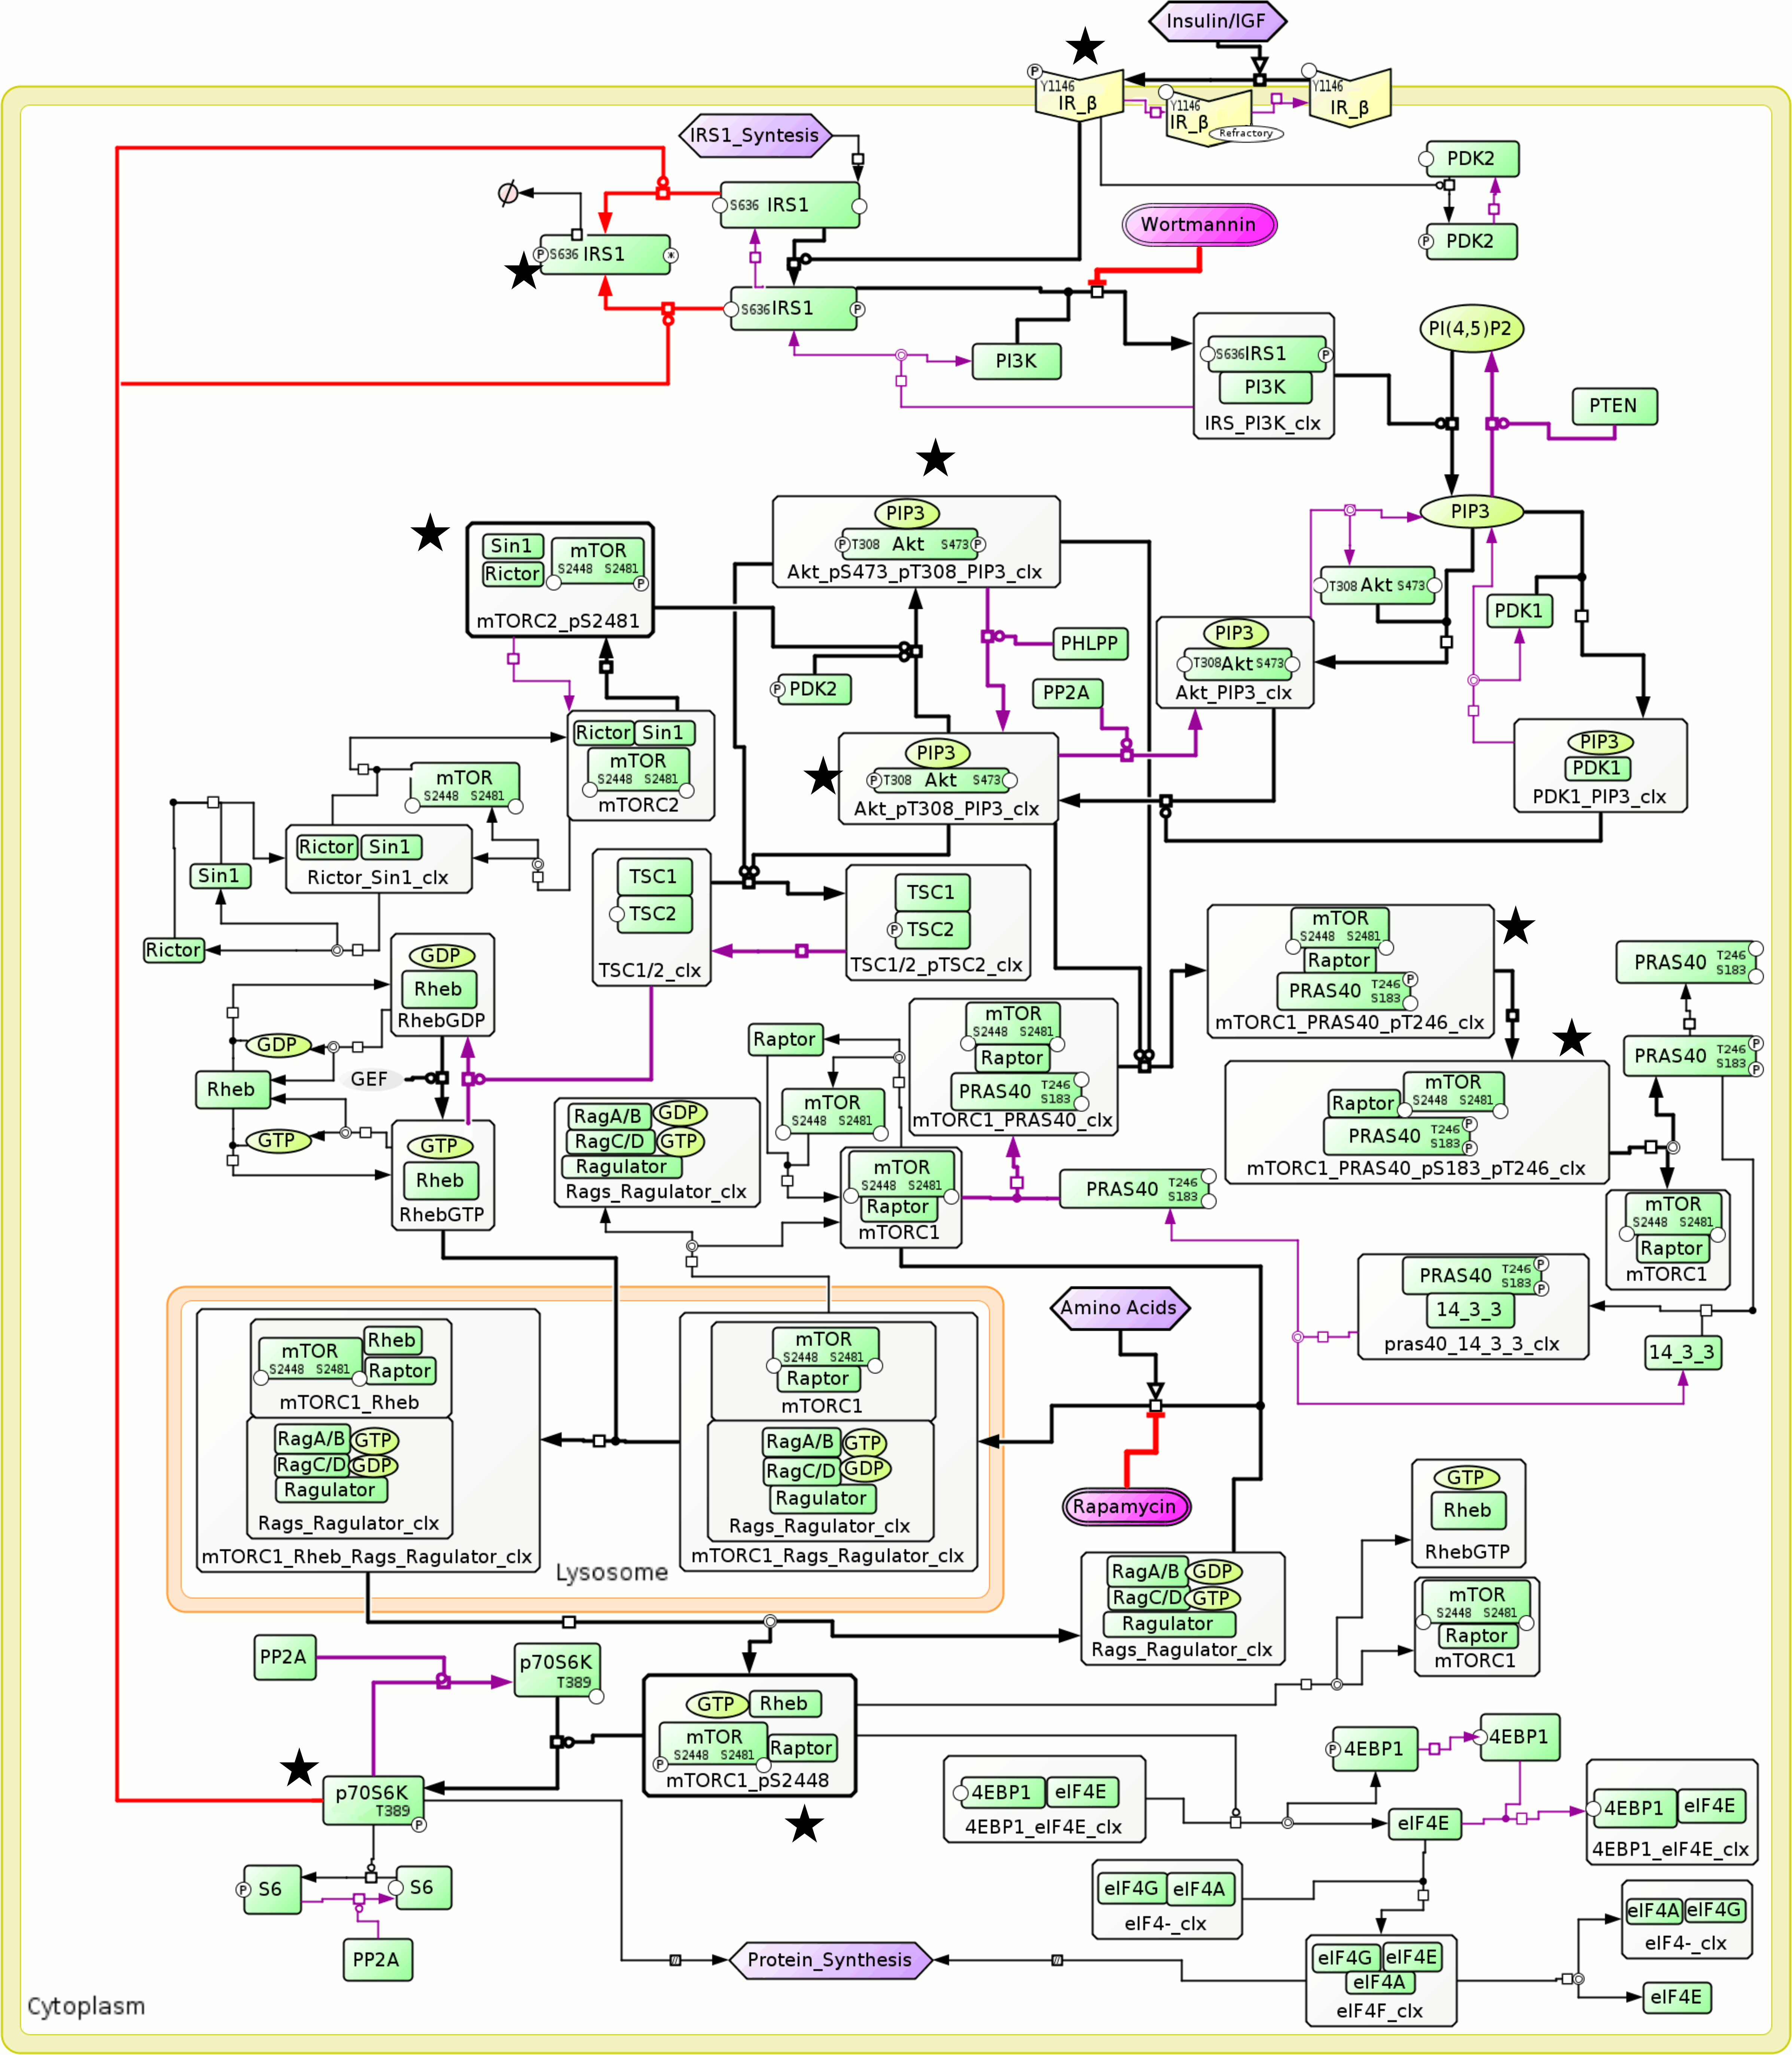
\includegraphics[width=5.7in, height=7.3in]{2002469_supp_fig1_improved.png}
		\caption[Extended graphical model of the mammalian TOR network]{A static network model of TOR signalling stimulated by amino acids plus insulin is shown in SBGN notation. This model integrates the current knowledge and guided our decision on appropriate targets for measurement. The selected targets are marked with an asterisk.}
		\label{fig:2002469_supp_fig1}
	\end{center}
\end{figure}
\clearpage

\begin{figure}[tb]
	\begin{center}
		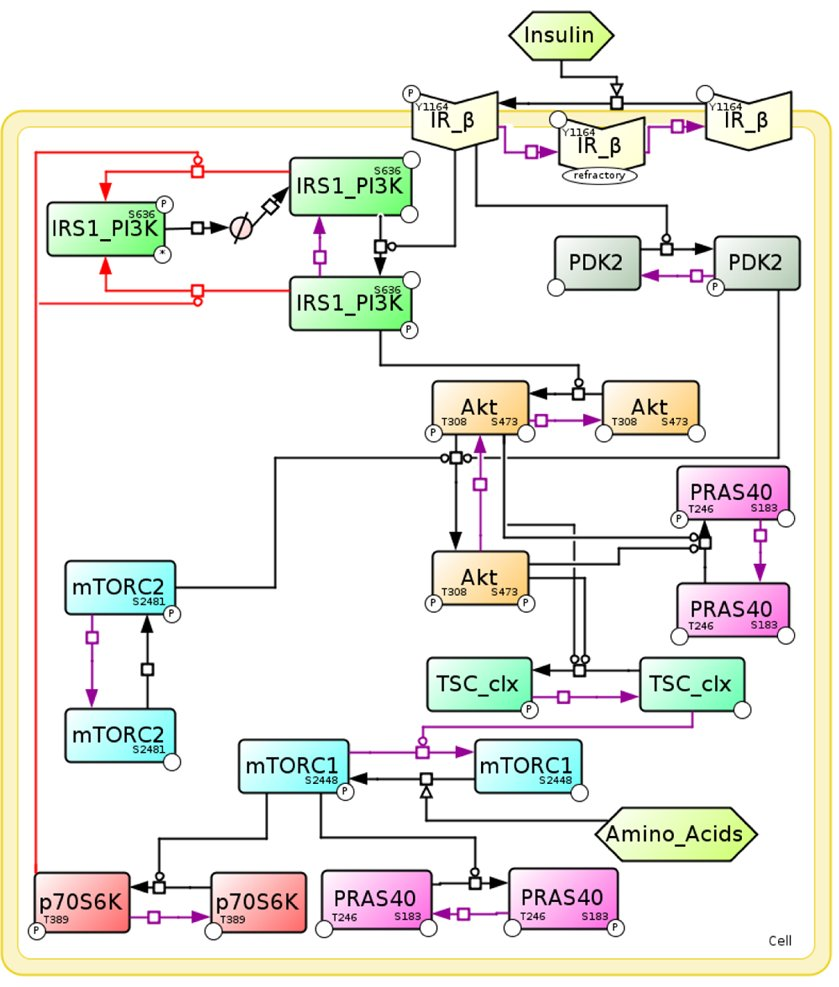
\includegraphics[scale=1.6]{2002469_fig1.jpg}
		\caption[An insulin/mTOR network graphical model]{An insulin/mTOR network graphical model. Reduced graphical model of the mTOR network activated by amino acids/insulin (see Figure \ref{fig:2002469_supp_fig1} for the extended graphical model).}
		\label{fig:2002469_fig1}
	\end{center}
\end{figure}
\clearpage

\begin{figure}[tb]
	\begin{center}
		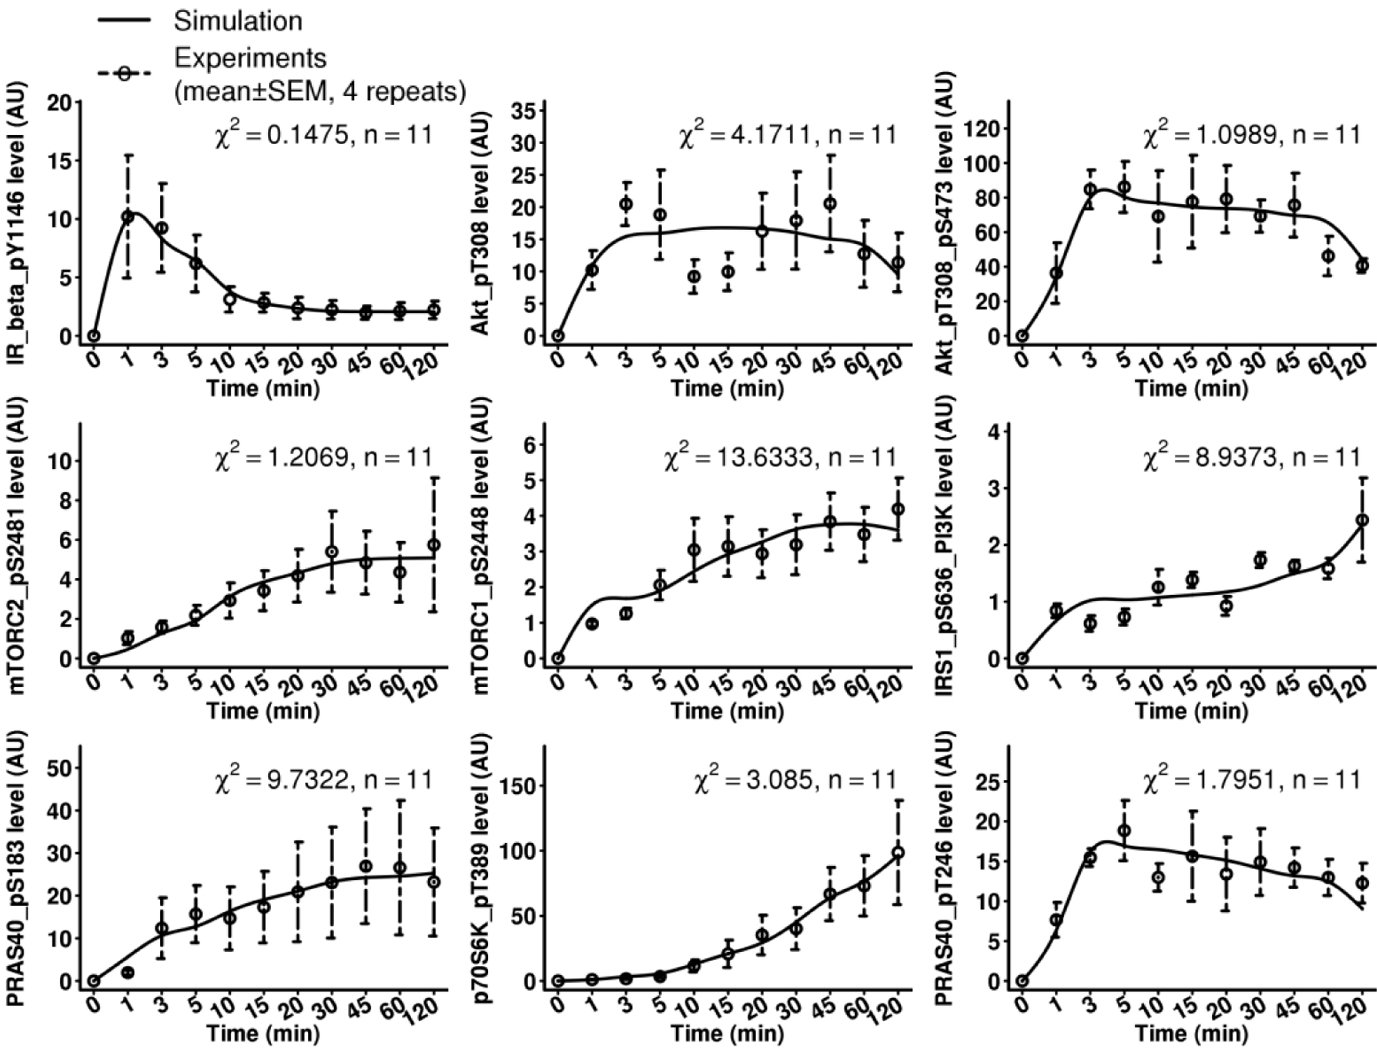
\includegraphics[scale=1.2]{2002469_fig2.jpg}
		\caption[Development of a dynamic insulin/mTOR network model]{Development of a dynamic insulin/mTOR network model. Comparison between the simulated time courses of the general model (solid lines) and the experimental time courses (points, dotted error bars) within [0, 120] min. For each curve, the $\chi^2$ computed over $n$ time points, is reported as goodness-of-fit measure. Experimental data based on quantitative immunoblotting time course by measuring phosphorylation dynamics of central network components (four replicates). \emph{In vitro} experiments were performed by Annika Sonntag, Freiburg University, Germany.}
		\label{fig:2002469_fig2}
	\end{center}
\end{figure}
\clearpage

\begin{figure}[tb]
	\begin{center}
		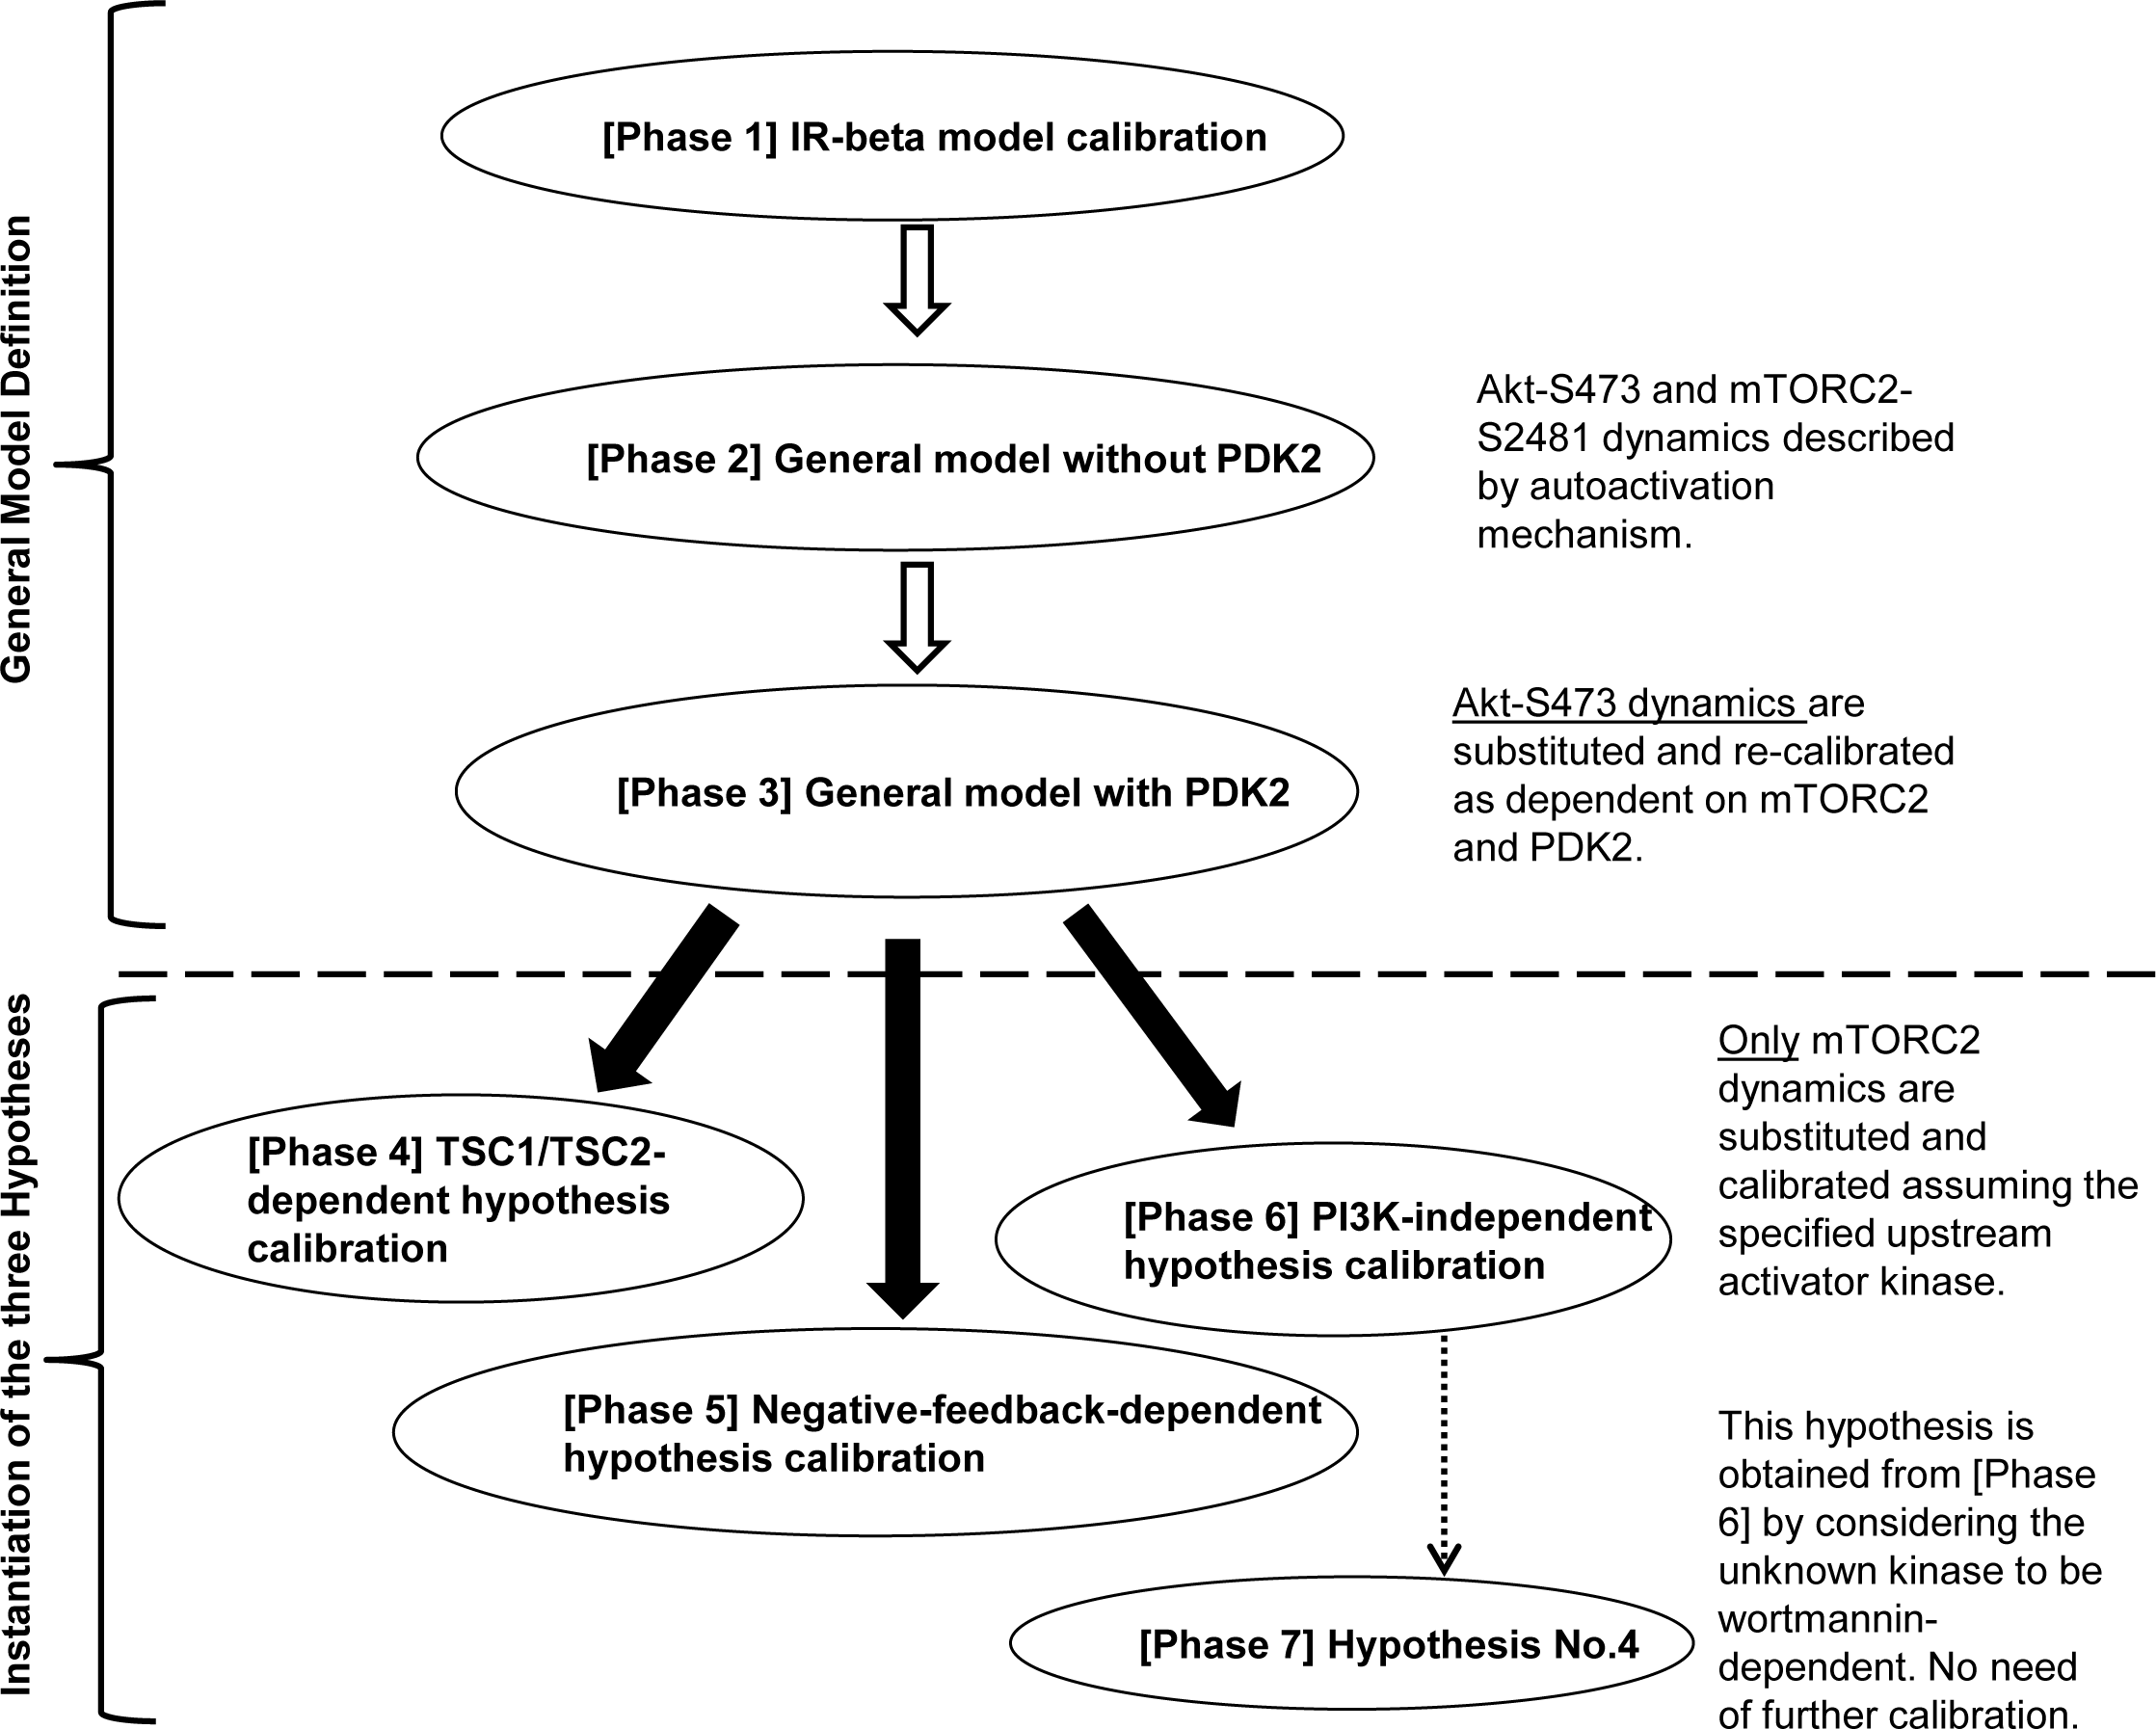
\includegraphics[scale=0.7]{2002469_supp_fig3.png}
		\caption[Phases of the calibration process]{Phases of the calibration process. The approach for defining our model was hierarchical and structured in two main parts. Part 1 (Phases 1-3) was the development of a general model without regulation of mTORC2 and Part 2 (Phases 4-7) was the introduction of specific hypotheses for regulation of mTORC2. In Phase 1, the kinetic rate constants of the insulin receptor were calibrated independently because the insulin receptor module was not regulated by the rest of the network. In Phase 2, the kinetic rate constants for the model representing the entire network without PDK2 were calibrated, assuming that the phosphorylation dynamics of mTOR-S2481 and Akt-S473 dynamics were regulated by autoactivation. In Phase 3, PDK2 was added to the network and the autoregulation mechanism controlling phosphorylation of Akt-S473 was replaced with the regulation by both mTORC2 and PDK2. Part 2 (Phases 4-7) of the calibration process concerned the introduction of the three hypotheses 
(Hypothesis 1,2, and 3) for mTORC2 activation from the general model defined in Part 1 (Phase 3). The development and calibration of these hypotheses only required substitution of the mTORC2 dynamics of the general model with the specific regulation of the corresponding hypothesis and then recalibration of these new kinetic parameters. In Phase 7, Hypothesis 4 was obtained from the PI3K-independent model by transforming the unknown kinase into one dependent on Wortmannin, which did not involve further calibration.}
		\label{fig:2002469_supp_fig3}
	\end{center}
\end{figure}
\clearpage

\begin{figure}[tb]
	\begin{center}
		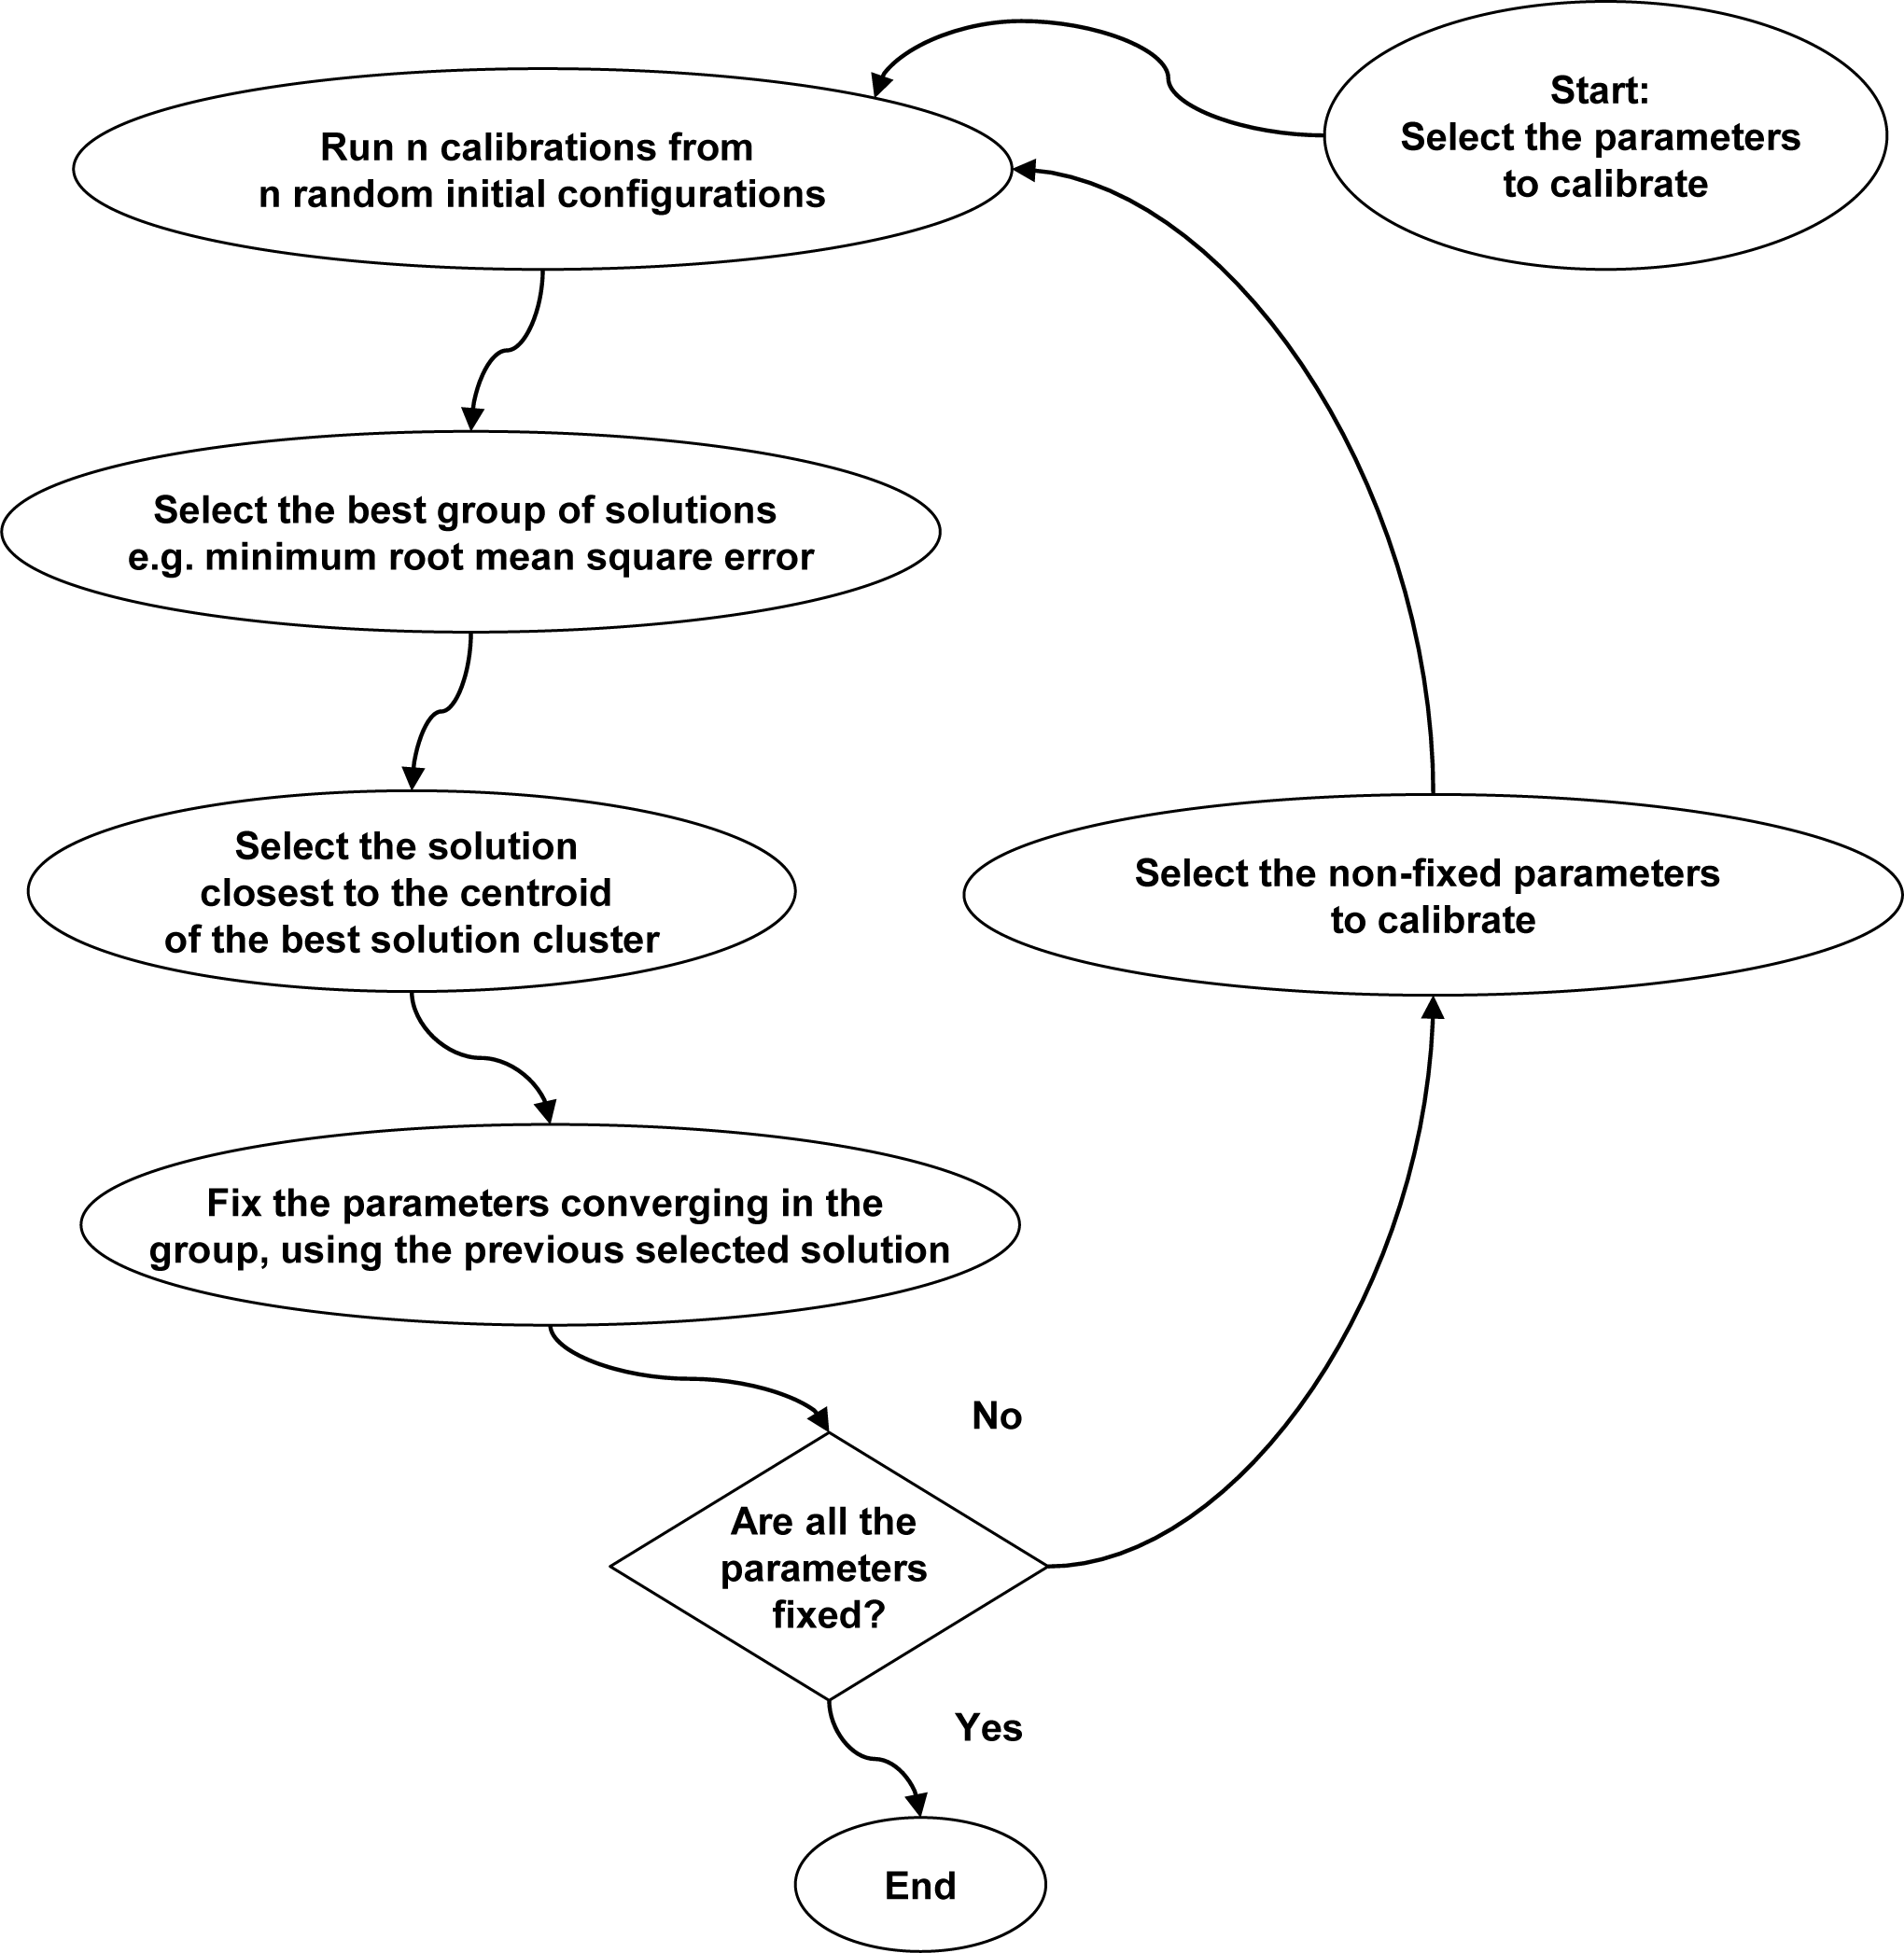
\includegraphics[scale=0.7]{2002469_supp_fig4.png}
		\caption[Detail of a calibration phase]{Detail of a calibration phase. The flow chart shows the details of the parameter calibration procedure. The procedure began with the selection of the set of parameters to estimate. After completing the calibrations, the procedure selected the subset of the solutions that obtained the minimum root mean square error (best solutions). The closest solution to the centroid of the best solution cluster was selected and the values common to all the solutions were fixed. All the parameters that were not fixed were selected for the next step of calibration. The procedure terminated when there were no further parameters to calibrate. In the model calibration, all the parameters were identified in only one iteration step.}
		\label{fig:2002469_supp_fig4}
	\end{center}
\end{figure}
\clearpage

\begin{figure}[tb]
	\begin{center}
		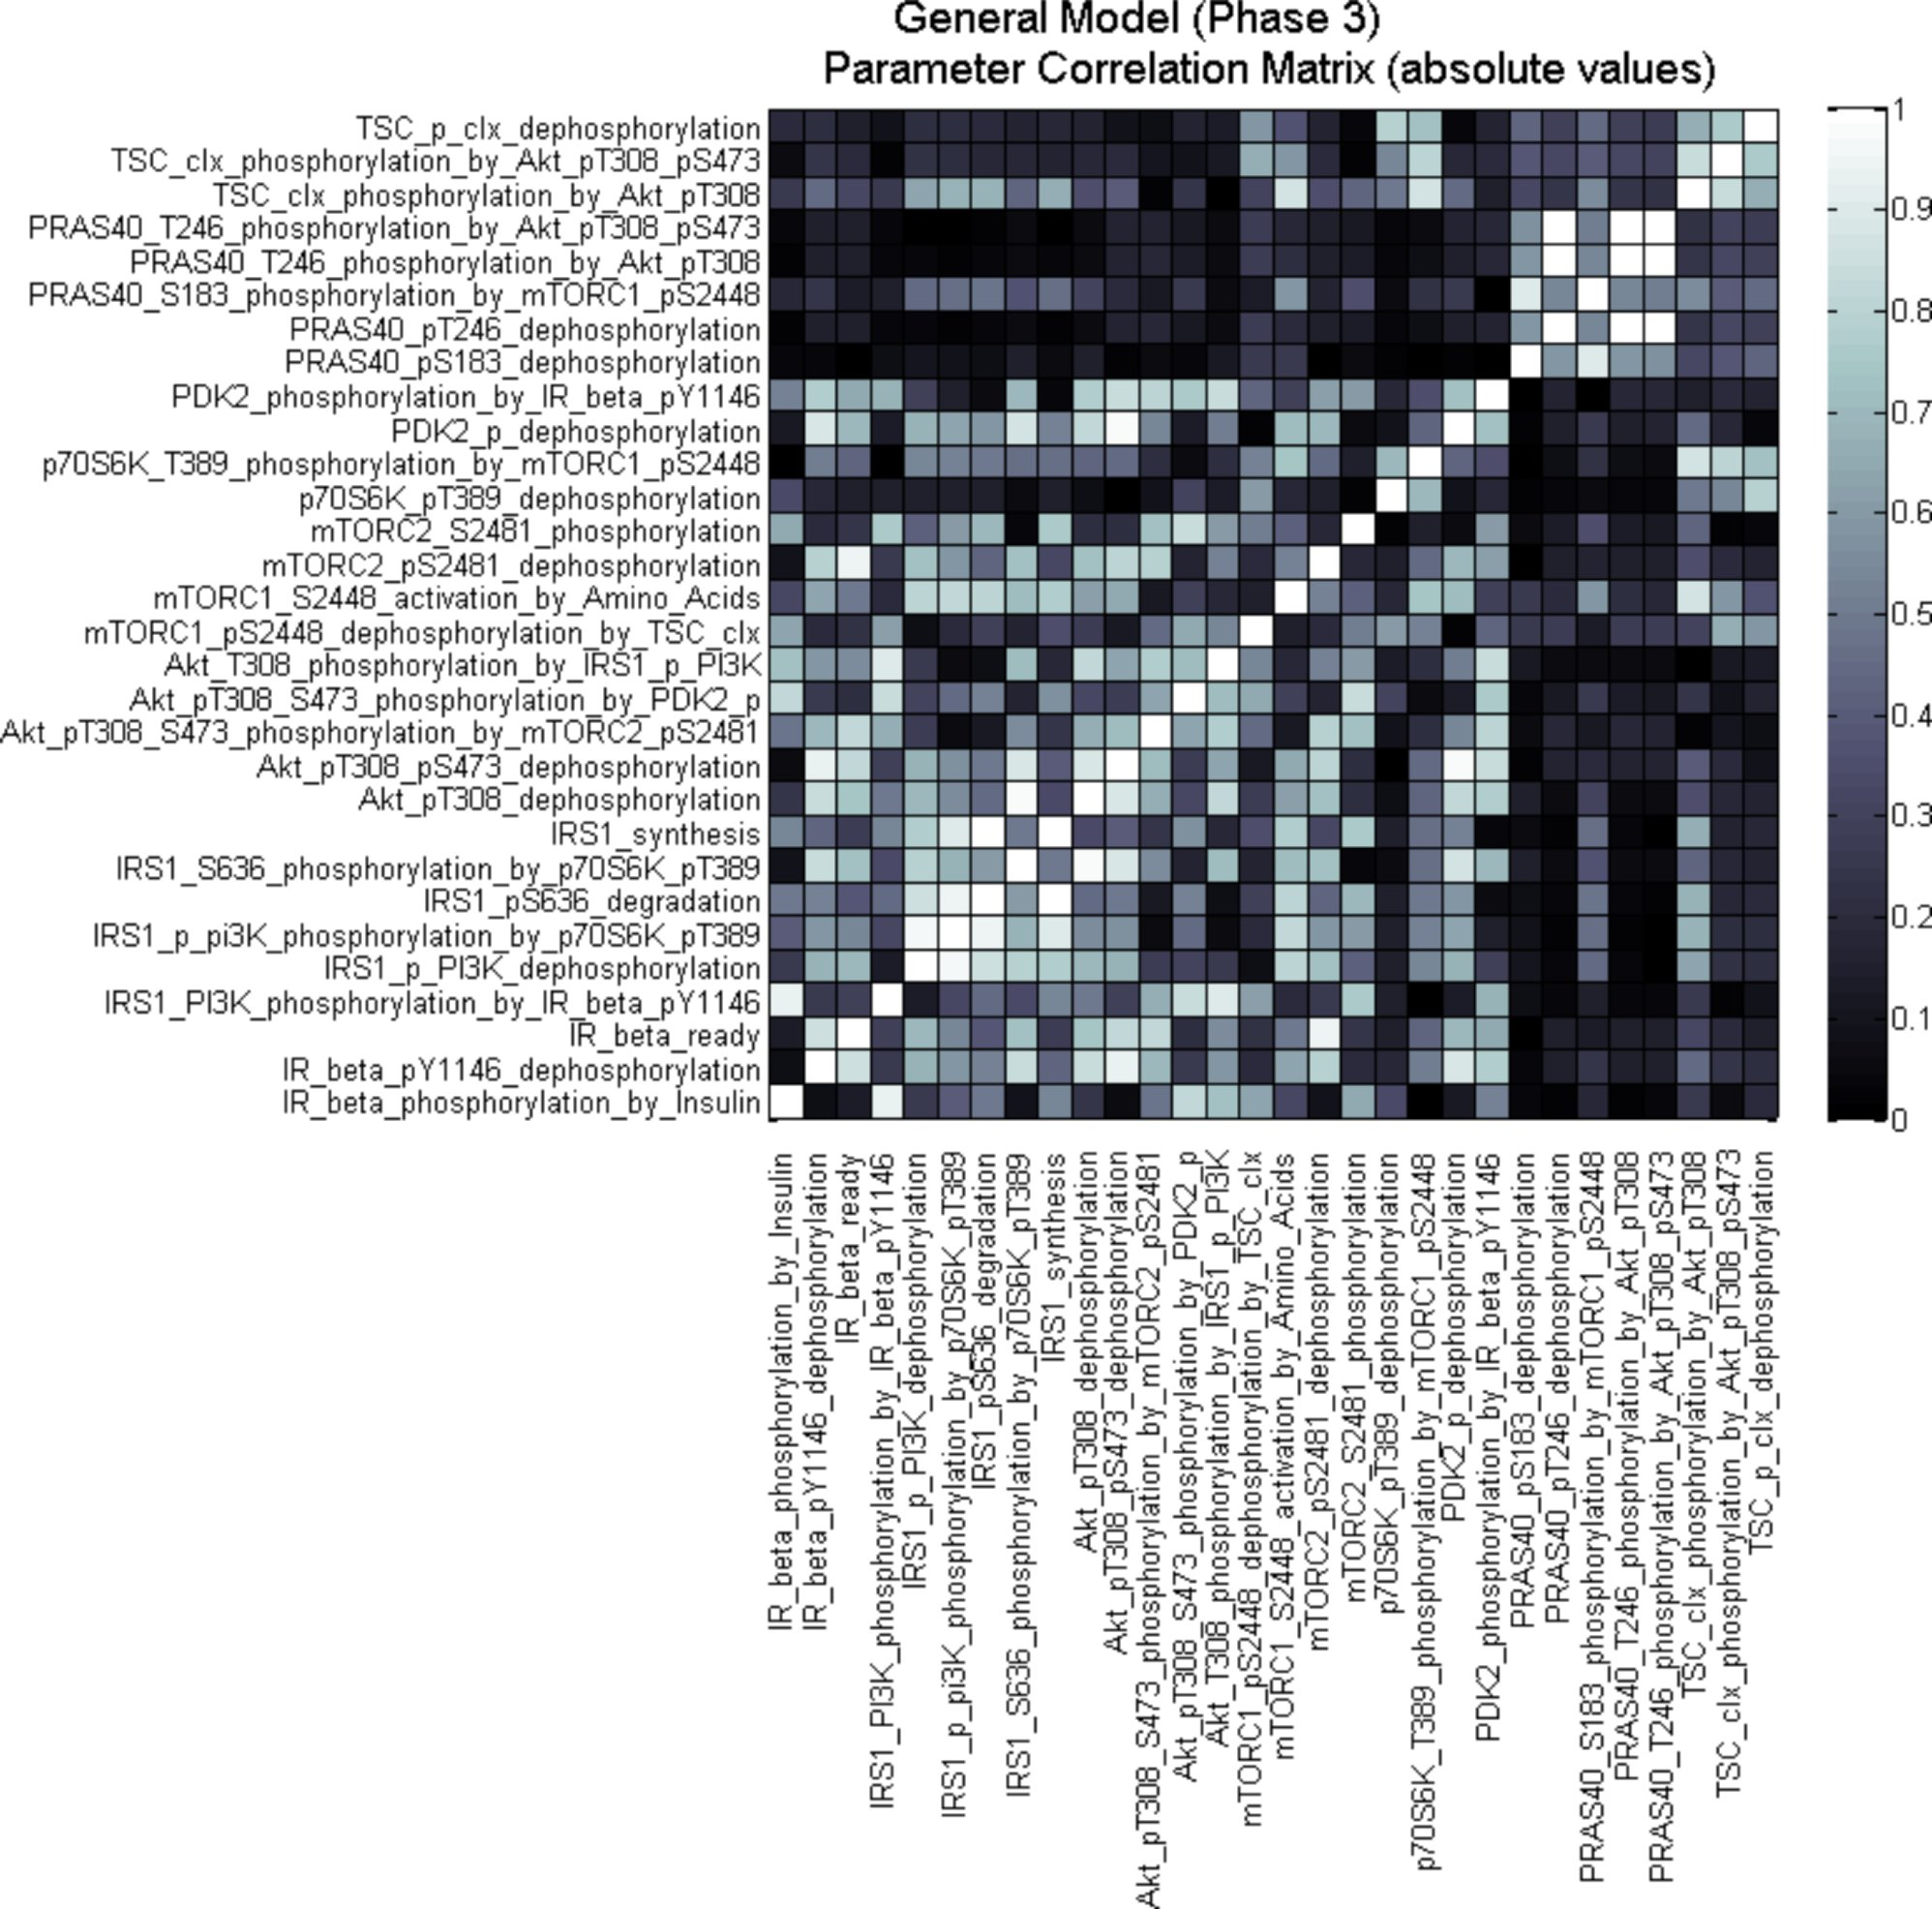
\includegraphics[scale=0.8]{2002469_supp_fig5.jpg}
		\caption[Identifiability analysis for the general model]{Identifiability analysis for the general model. Parameter identifiability is based on sensitivity analysis and parameter correlation as computed by SBPD Matlab Toolbox. The symmetric matrix shows the parameter correlation in absolute values. High parameter correlations suggest potential issues in identifying the corresponding parameters independently (the elements on the diagonal obviously have correlation equal to 1). Conversely, low parameter correlations indicate that the corresponding parameters can be identified independently. Our experimental data were used in computing the reported identifiability analysis.}
		\label{fig:2002469_supp_fig5}
	\end{center}
\end{figure}
\clearpage

\begin{figure}[tb]
	\begin{center}
		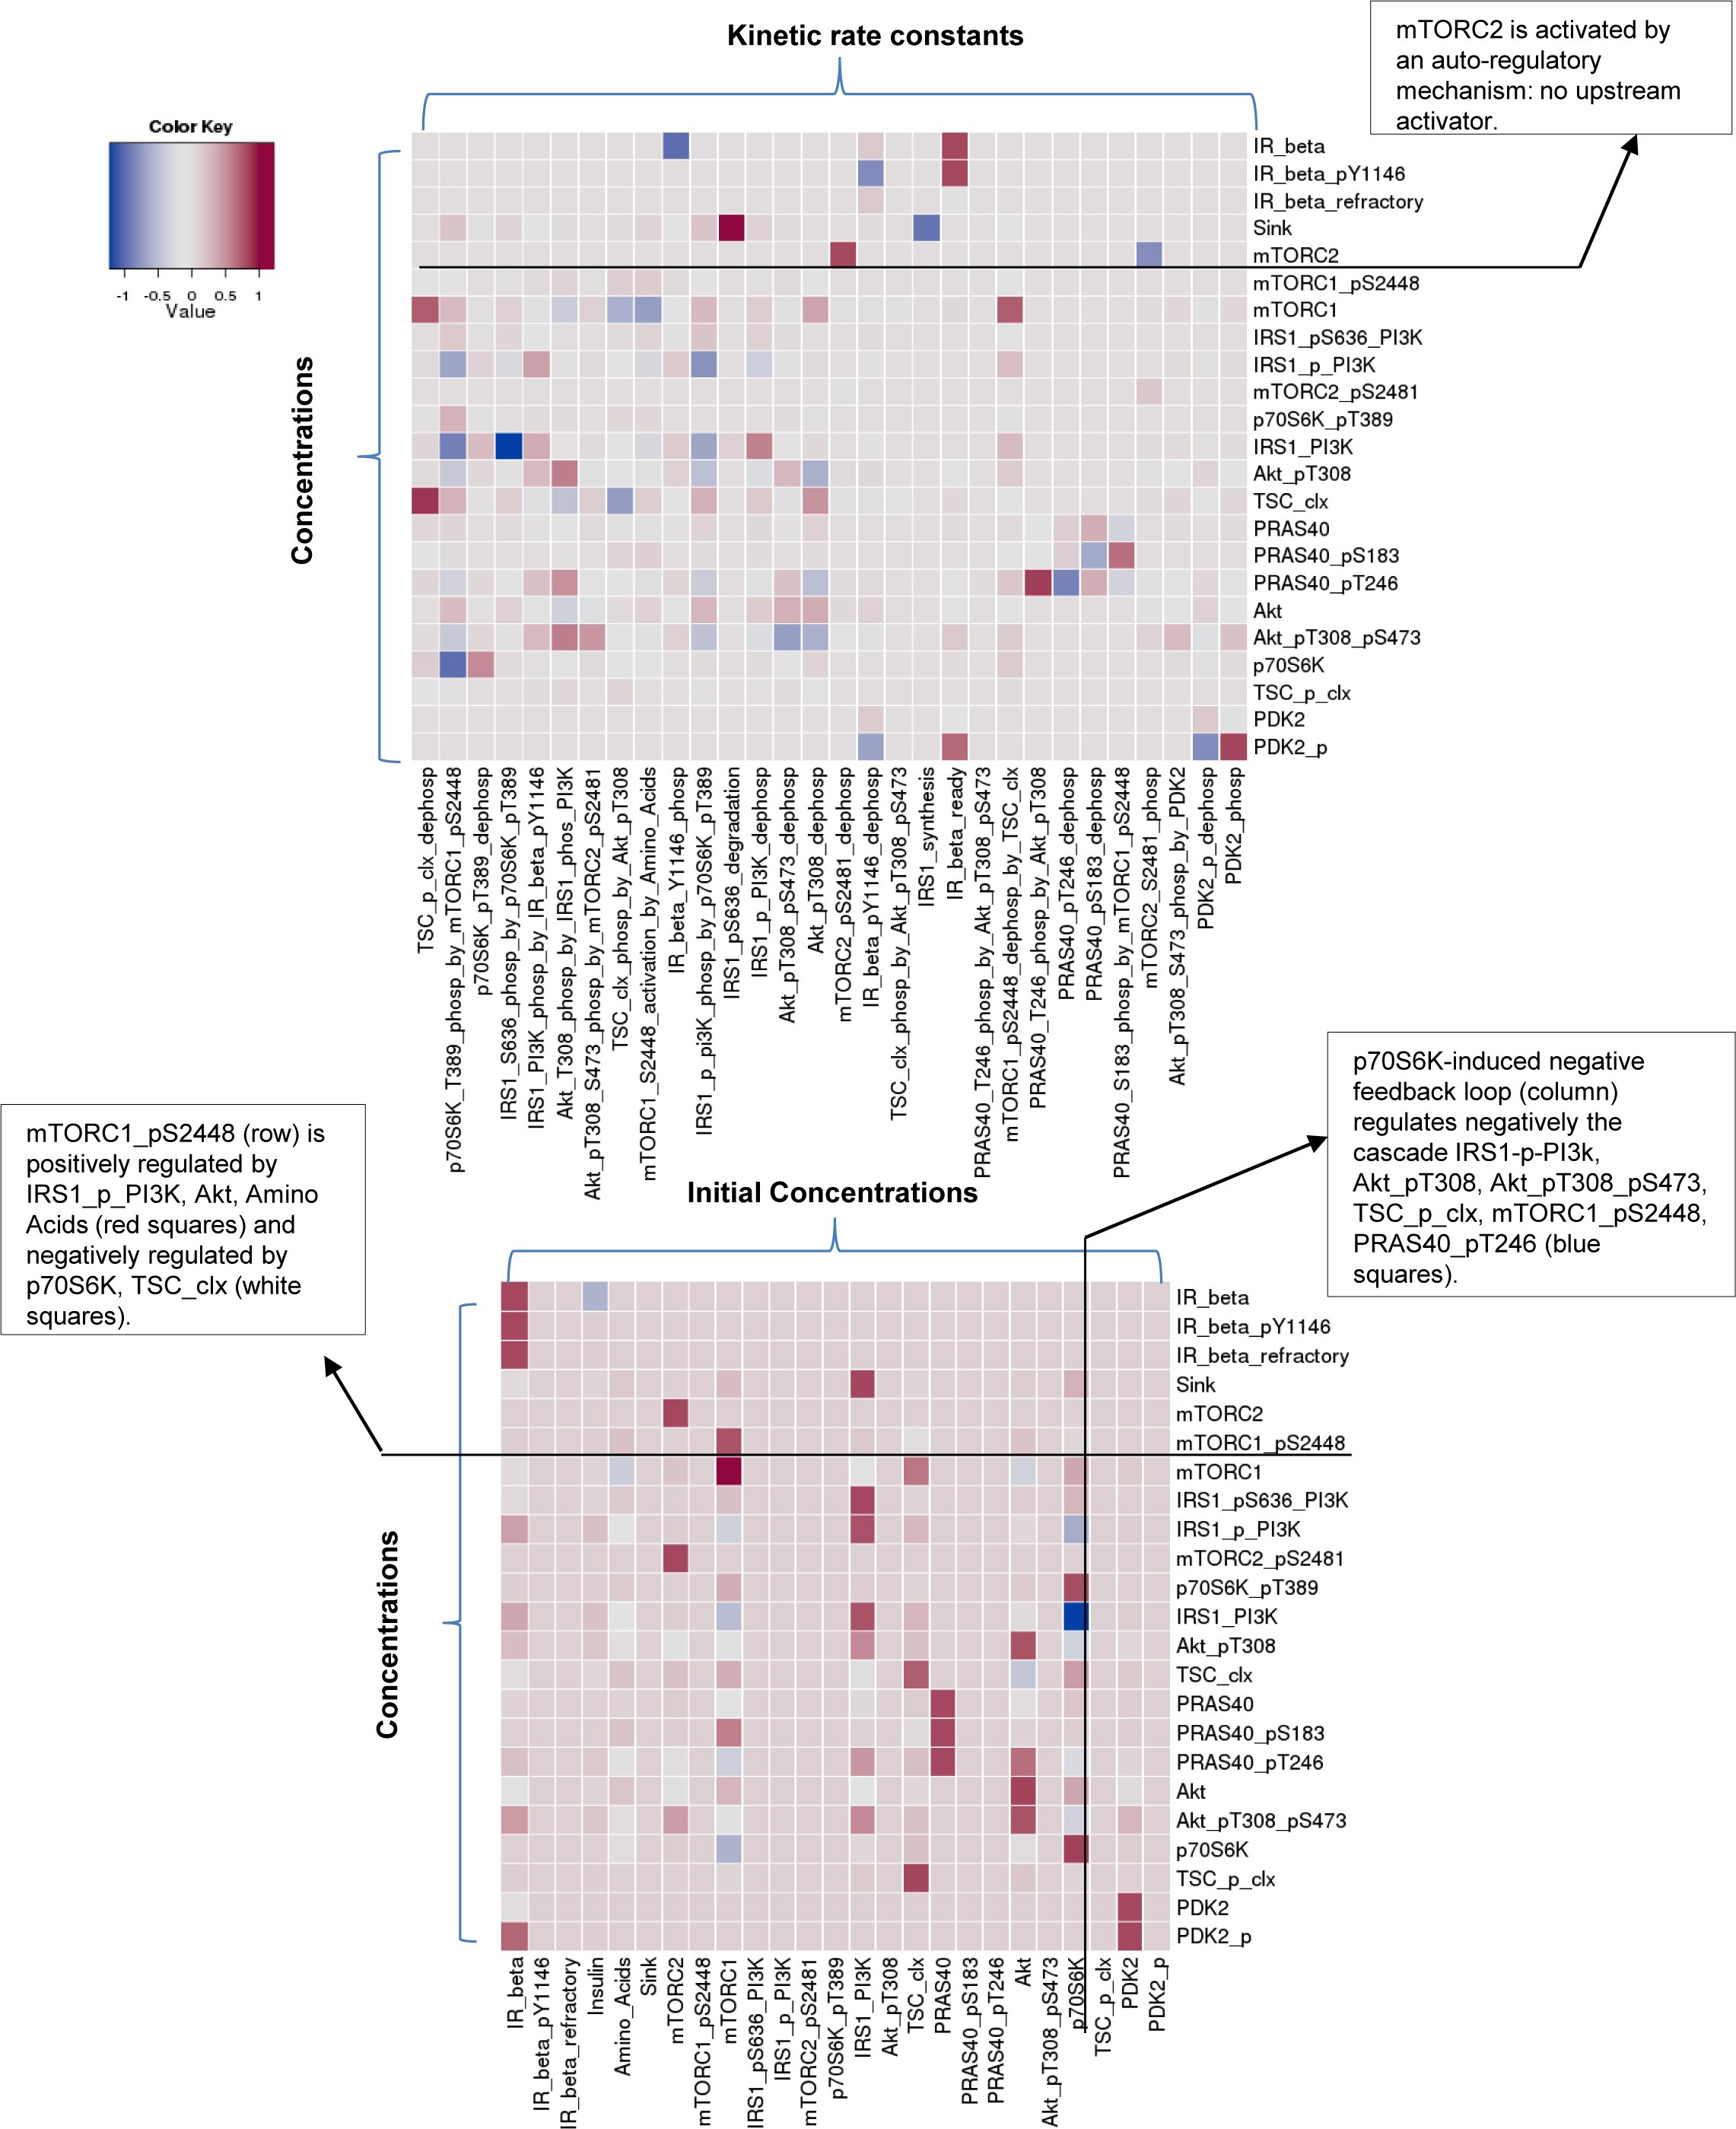
\includegraphics[width=5.60in]{2002469_supp_fig6.jpg}
		\caption[Sensitivity analysis for the general model]{Sensitivity analysis for the general model. The top plot illustrates the sensitivity analysis of the model by row, in response to the perturbations of the kinetic rates constants shown in columns. The bottom plot shows the model sensitivity analysis of the initial concentrations of the modelled species by row with perturbations shown in columns. Values were normalised in the range [-1, 1]. Positive values (red squares) represent positive regulation; negative ones (white-blue squares) represent inhibition.}
		\label{fig:2002469_supp_fig6}
	\end{center}
\end{figure}
\clearpage

\begin{figure}[tb]
	\begin{center}
		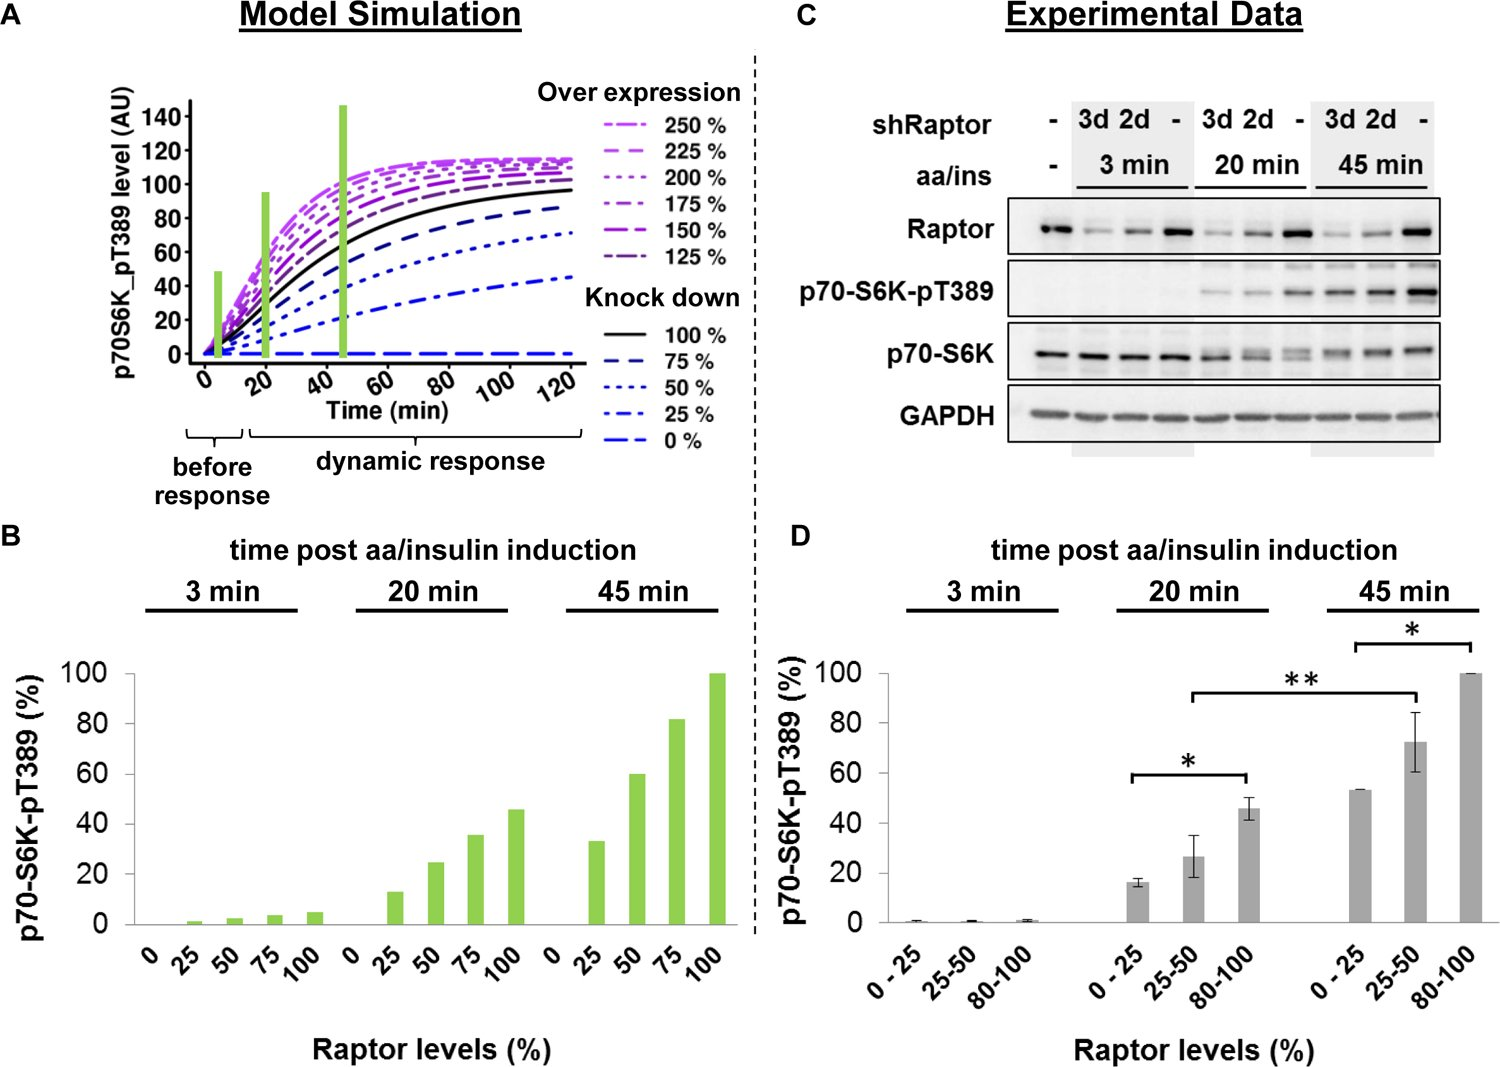
\includegraphics[scale=1.05]{2002469_fig3.jpg}
		\caption[Validation: dynamic response of p70-S6K-pT389 to gradual Raptor inhibition]{Validation: dynamic response of p70-S6K-pT389 to gradual Raptor inhibition. (A) Model predictions for p70-S6K-pT389 dynamics in response to a perturbation of mTORC1. The curves show the simulated response to gradual mTORC1 inhibition starting at 5-10 minutes after induction with amino acids/insulin. The model was simulated with both mTORC1 overexpression and knockdown conditions. Time points for experimental validation are indicated by green lines. (B) Simulated and quantified relative amounts of p70-S6K-pT389 under conditions of mTORC1 reduction (0, 25, 50, 75, 100 \%) at selected time points after induction with amino acids/insulin. (C) Experimental validation of the effect of gradual Raptor knockdown (shRaptor) on p70-S6K phosphorylation in starved cells induced with amino acids/ins for the indicated times. Data are representative of 3 experiments. d = days. (D) Experimentally determined and quantified p70-S6K-pT389 
amounts at the indicated times after induction with amino acids/insulin in cells in which Raptor was knocked down. Data are the average and SEM of 3 experiments. * $P\;<\;0.05$, ** $P\;<\;0.01$; low Raptor levels compared to high Raptor levels after 20 min and 45 min induction, 20 min compared to 45 min induction.  Differences in p70-S6K-pT389 were significant. \emph{In vitro} experiments were performed by Annika Sonntag, Freiburg University, Germany.}
		\label{fig:2002469_fig3}
	\end{center}
\end{figure}
\clearpage

\begin{figure}[tb]
	\begin{center}
		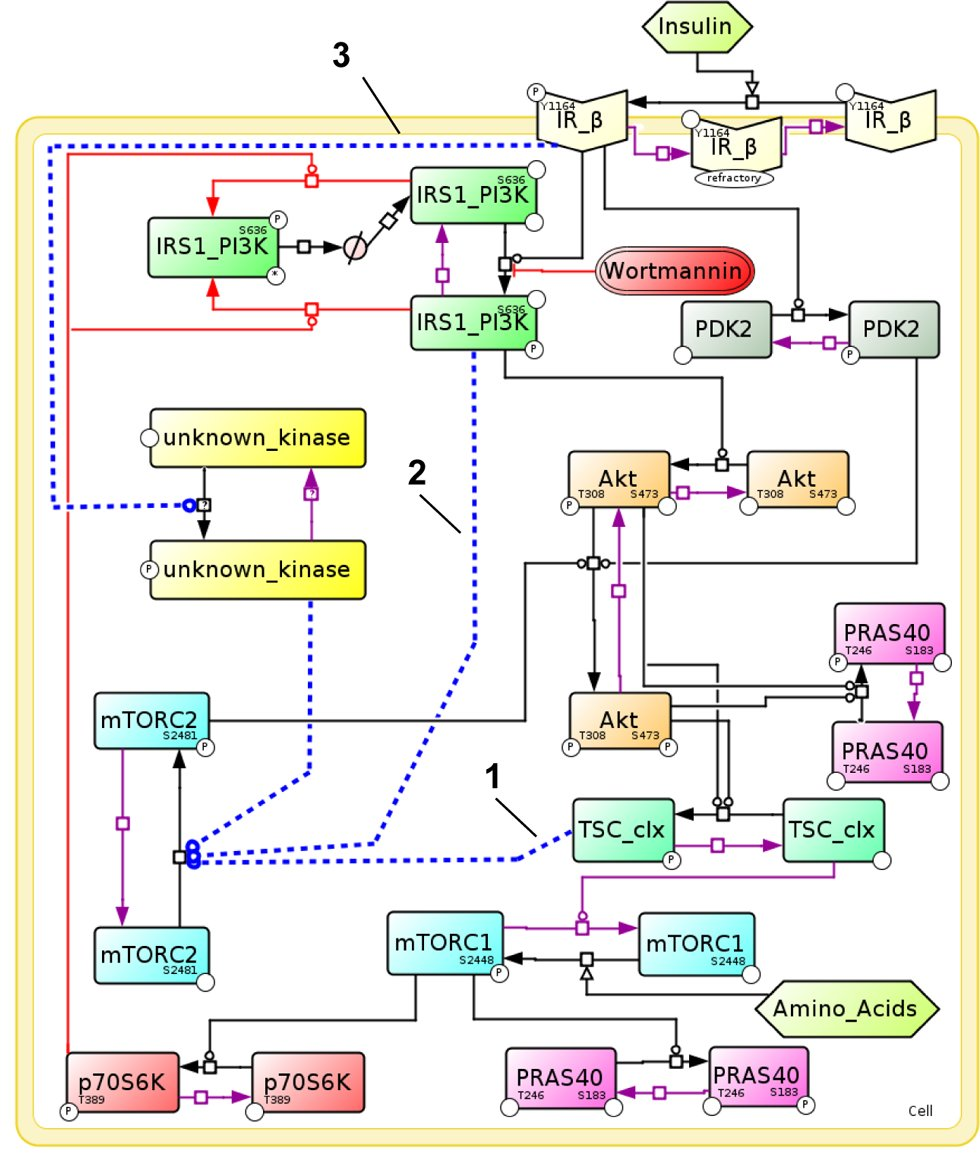
\includegraphics[scale=1.4]{2002469_fig4B.jpg}
		\caption[Three different hypotheses on mTORC2 regulation by insulin (graphical model)]{Three different hypotheses on mTORC2 regulation by insulin (graphical model). Reduced graphical network model including the three hypotheses (1, 2, 3, indicated by the dotted lines), translated into different network structures.}
		\label{fig:2002469_fig4B}
	\end{center}
\end{figure}
\clearpage

\begin{figure}[tb]
	\begin{center}
		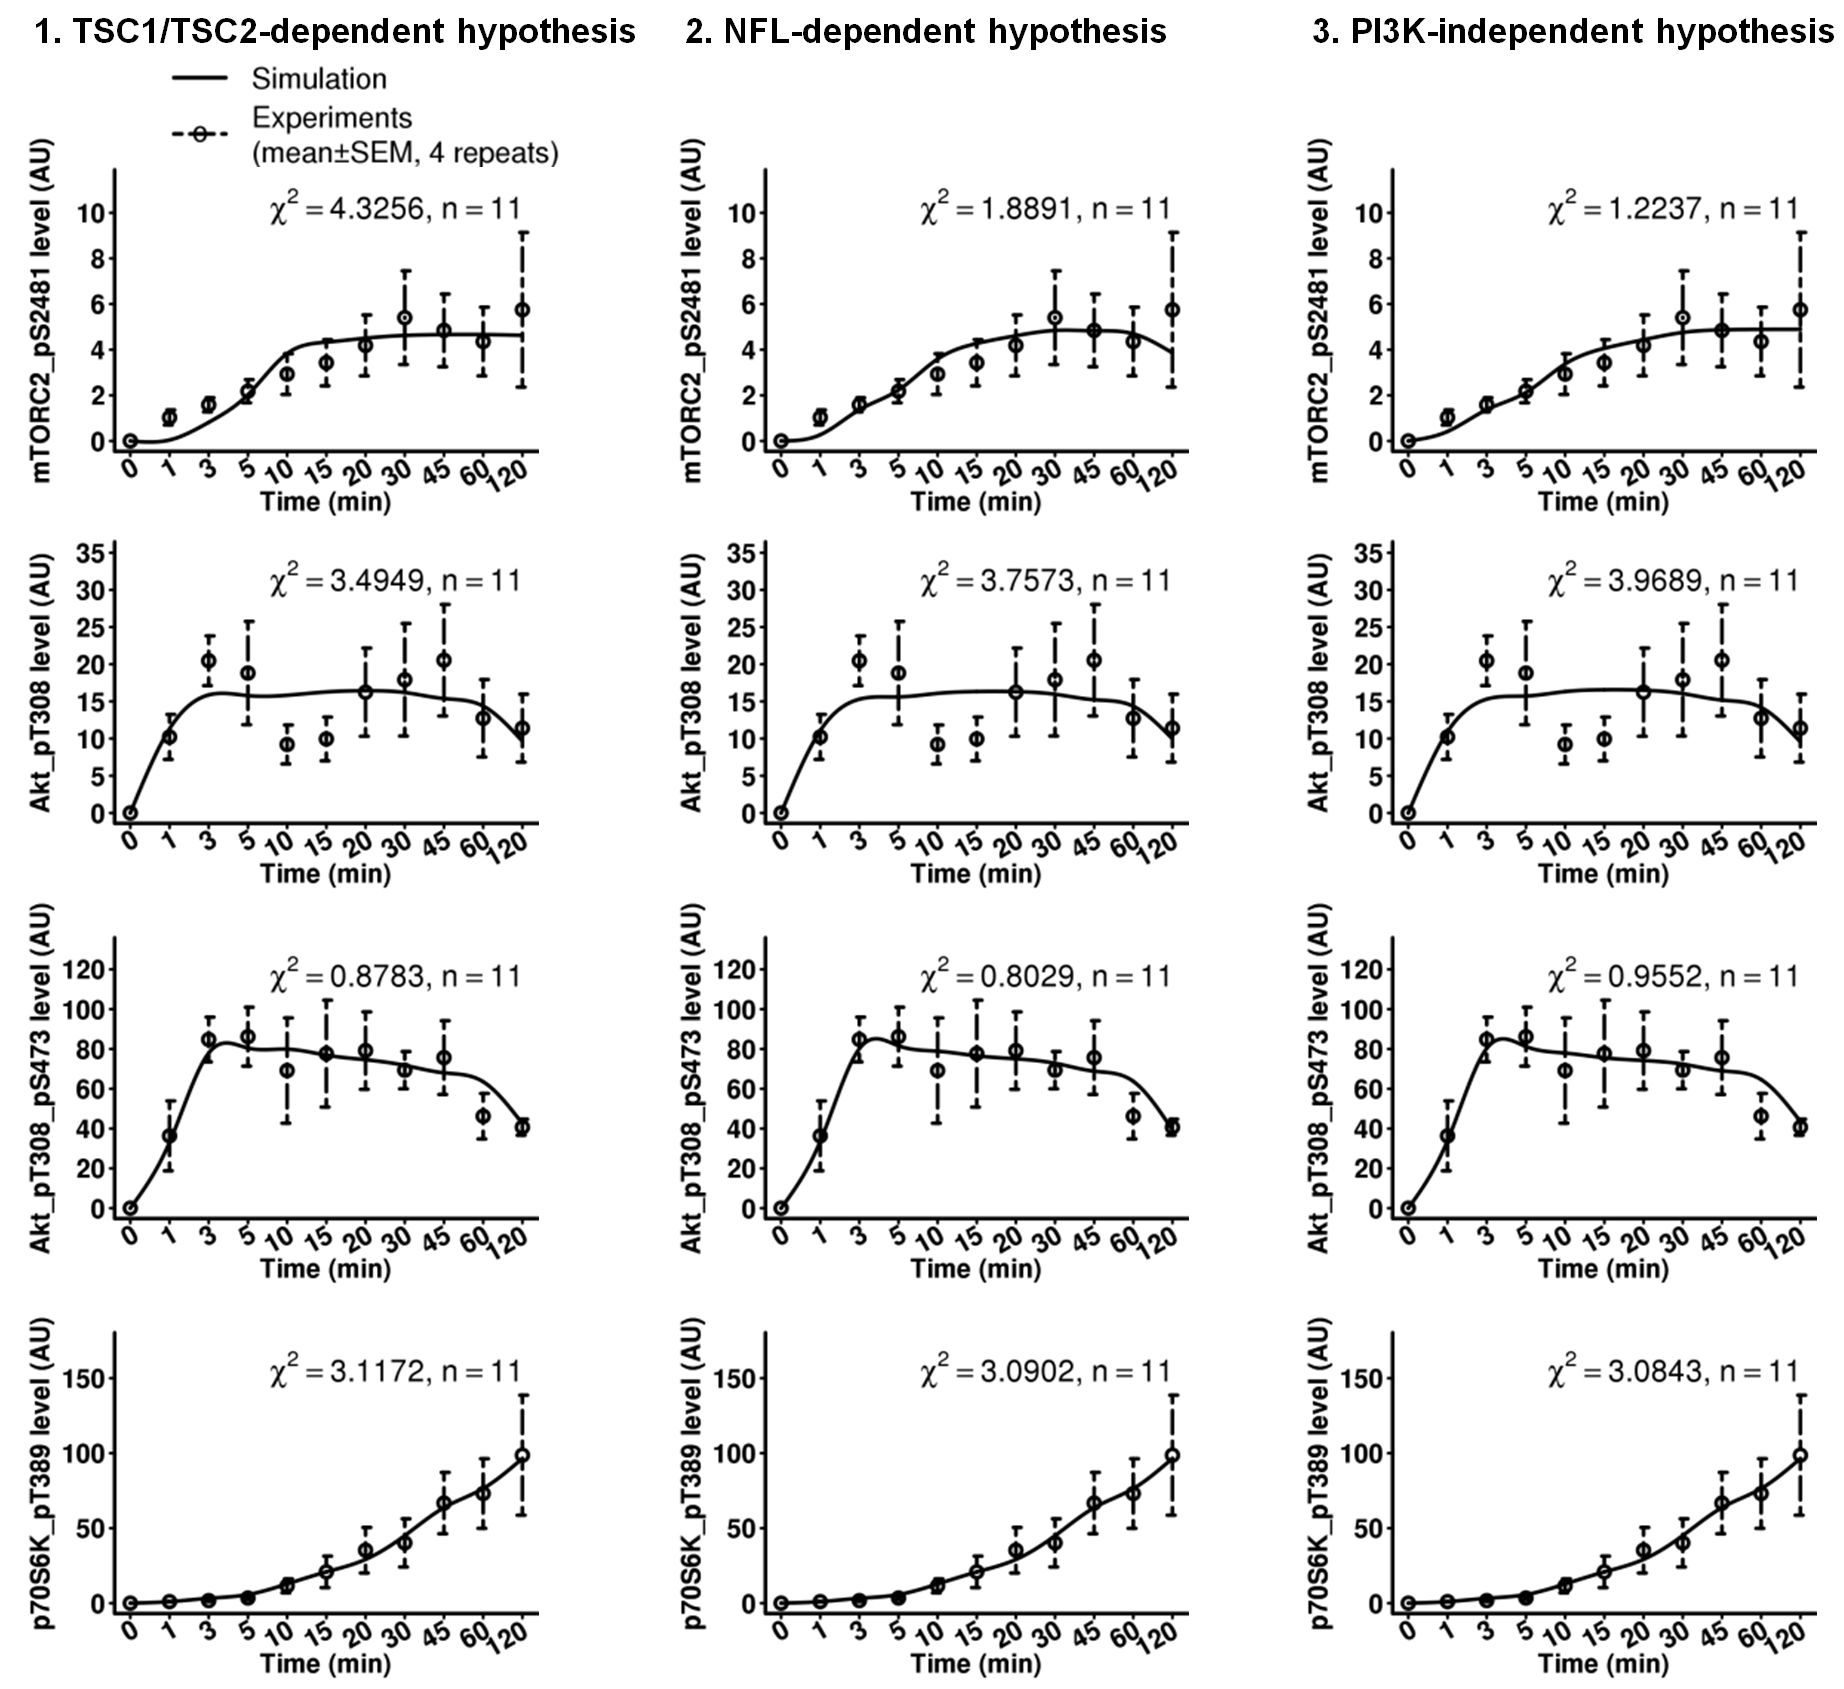
\includegraphics[scale=0.8]{2002469_fig4C.png}
		\caption[Three different hypotheses on mTORC2 regulation by insulin (dynamical models)]{Three different hypotheses on mTORC2 regulation by insulin (dynamical models). Comparisons of simulated time courses, calibrated for each hypothesis, with experimental data. Data shown are for mTORC2 readouts (mTOR-pS2481, Akt-pS473), the PI3K readout Akt-pT308, and the mTORC1 readout p70-S6K-pT389 (see Figure \ref{fig:2002469_supp_fig7} for curves of all other readouts). \emph{In vitro} experiments were performed by Annika Sonntag, Freiburg University, Germany.}
		\label{fig:2002469_fig4C}
	\end{center}
\end{figure}
\clearpage

\begin{figure}[tb]
	\begin{center}
		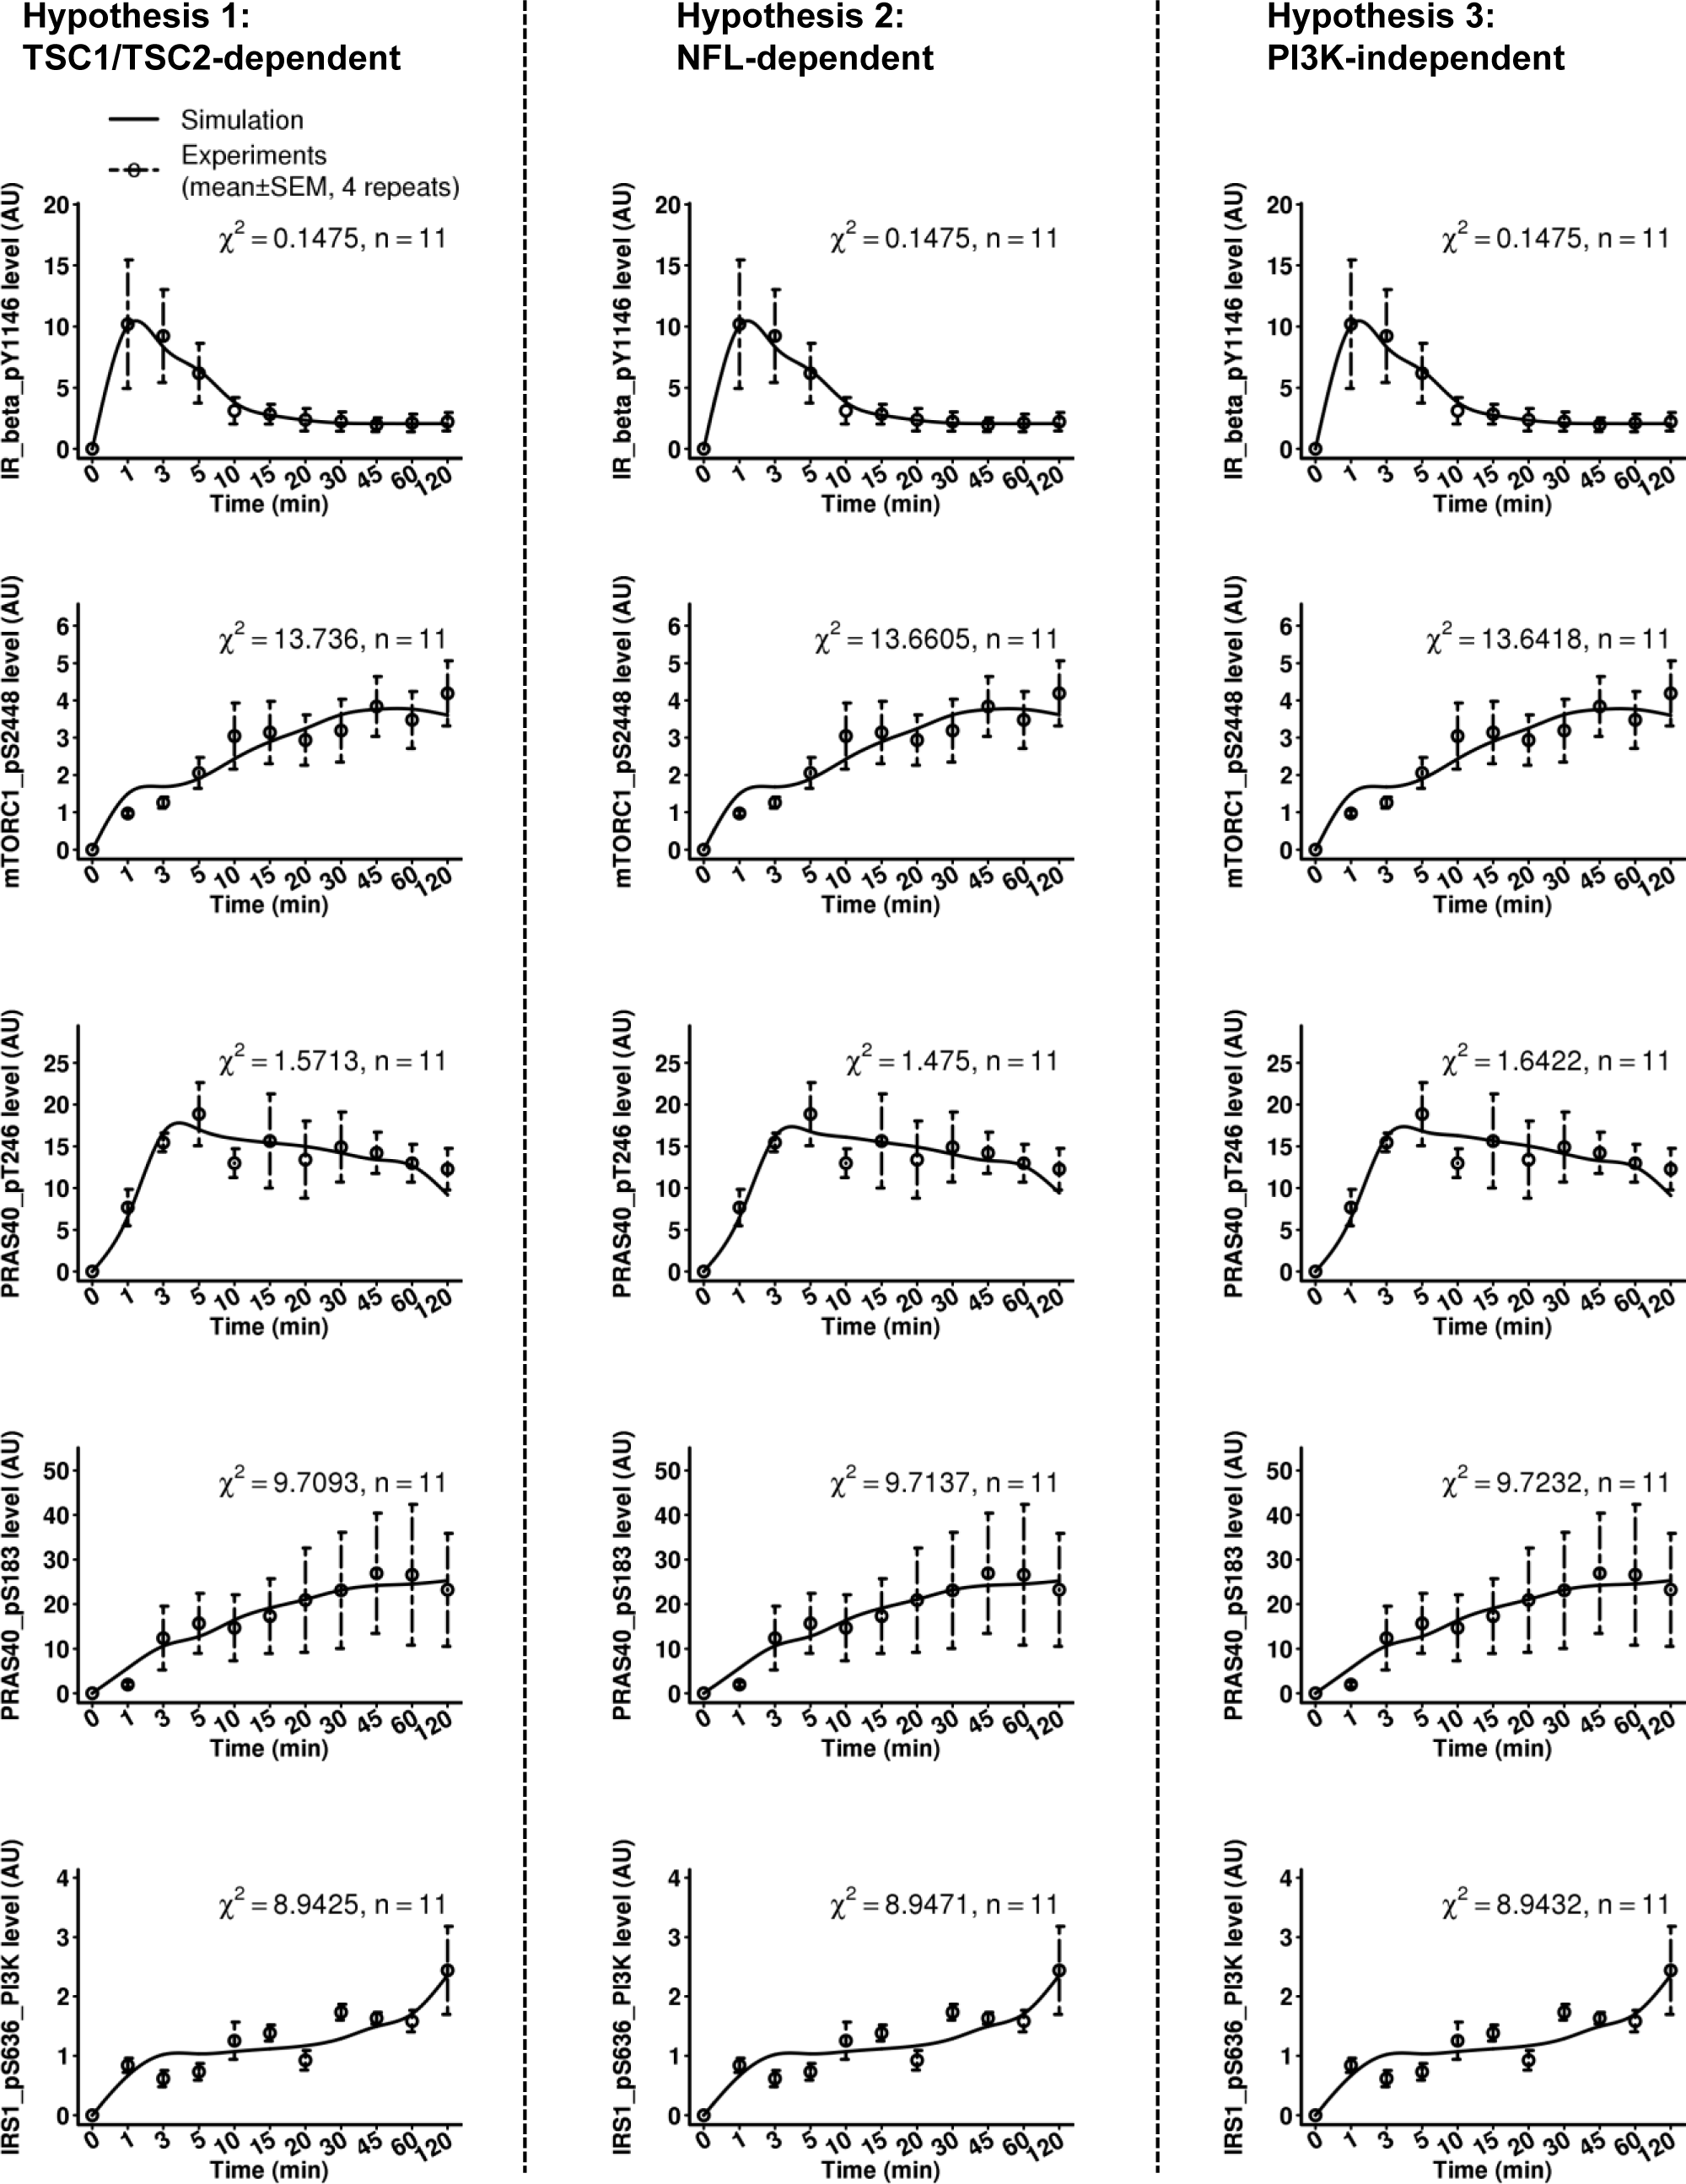
\includegraphics[scale=0.8]{2002469_supp_fig7.png}
		\caption[Comparison between the simulated and experimental time-courses for Hypotheses 1, 2, and 3 for readouts of the mTOR network]{Comparison between the simulated and experimental time-courses for Hypothesis 1, 2, and 3 for readouts of the mTOR network. The three hypotheses were consistent with each other for all the readouts indicating that introducing each hypothesis into the general model did not perturb the network. NFL = Negative Feedback Loop. \emph{In vitro} experiments were performed by Annika Sonntag, Freiburg University, Germany.}
		\label{fig:2002469_supp_fig7}
	\end{center}
\end{figure}
\clearpage

\begin{figure}[tb]
	\begin{center}
		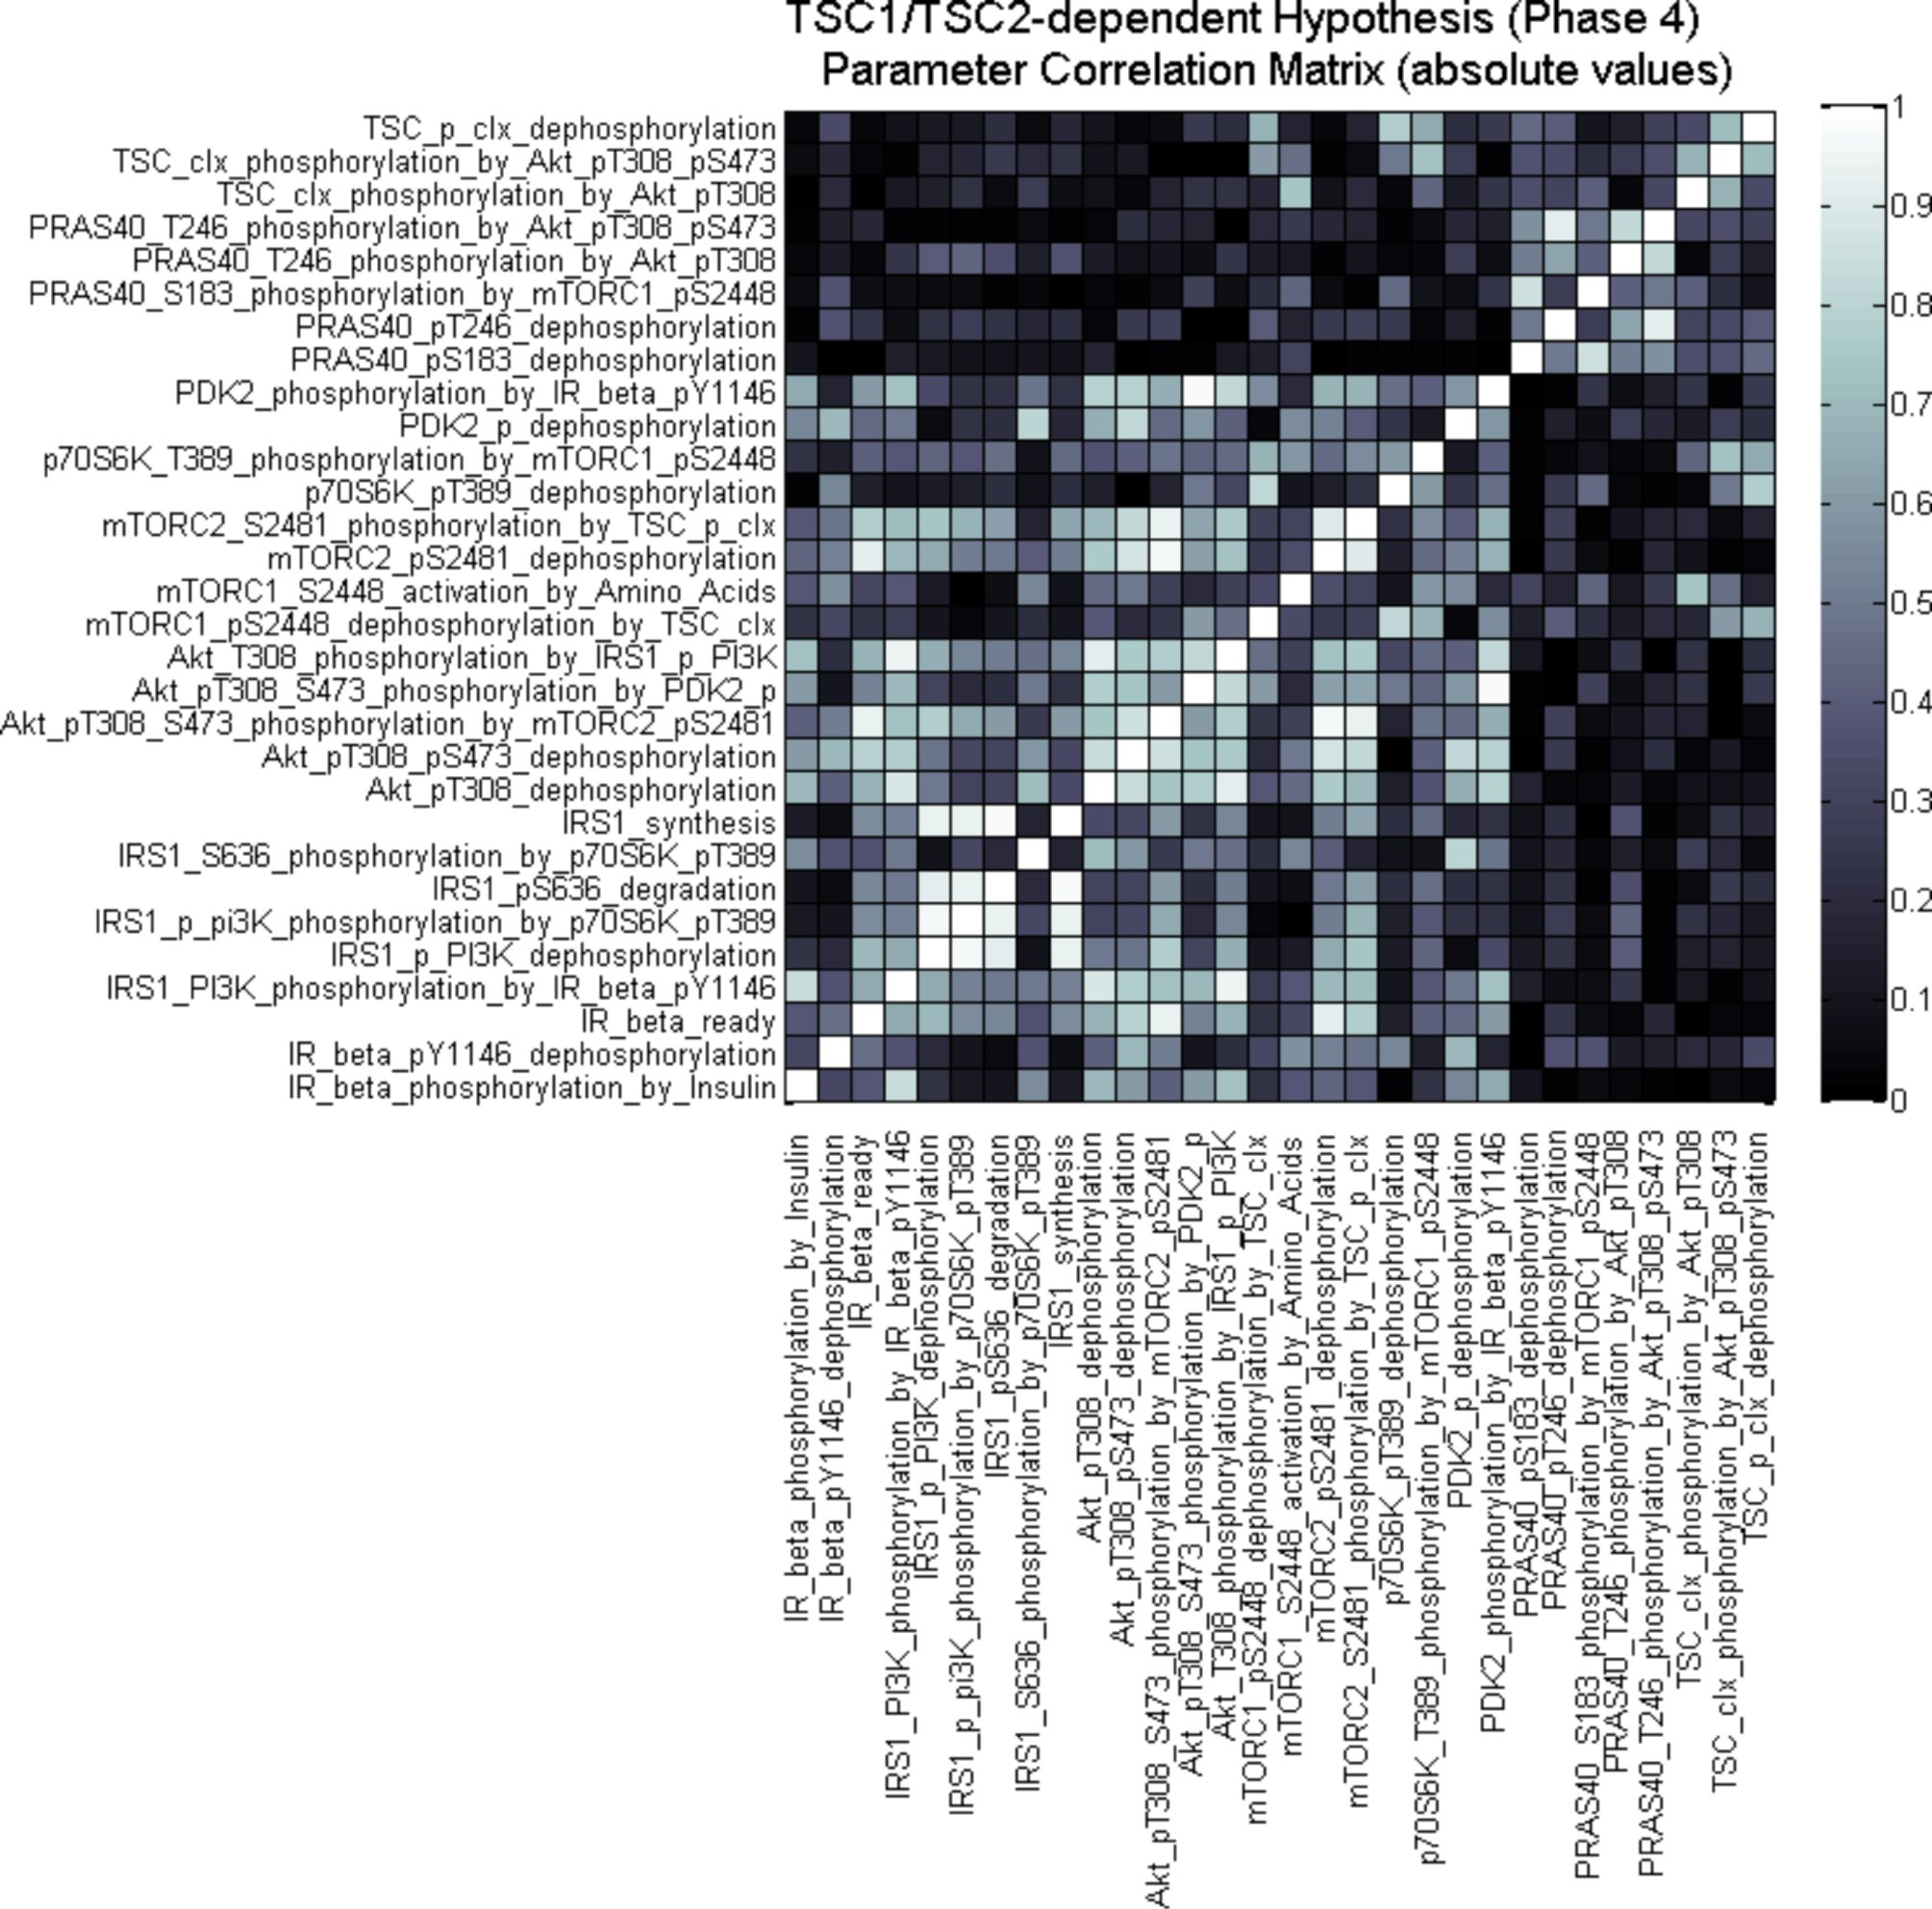
\includegraphics[scale=0.8]{2002469_supp_fig8.jpg}
		\caption[Identifiability analysis for Hypothesis 1: TSC1/TSC2-dependent mTORC2 regulation]{Identifiability analysis for Hypothesis 1: TSC1/TSC2-dependent mTORC2 regulation. Parameter correlation matrix for TSC1/TSC2-dependent hypothesis is shown. See Figure \ref{fig:2002469_supp_fig5} for details.}
		\label{fig:2002469_supp_fig8}
	\end{center}
\end{figure}
\clearpage

\begin{figure}[tb]
	\begin{center}
		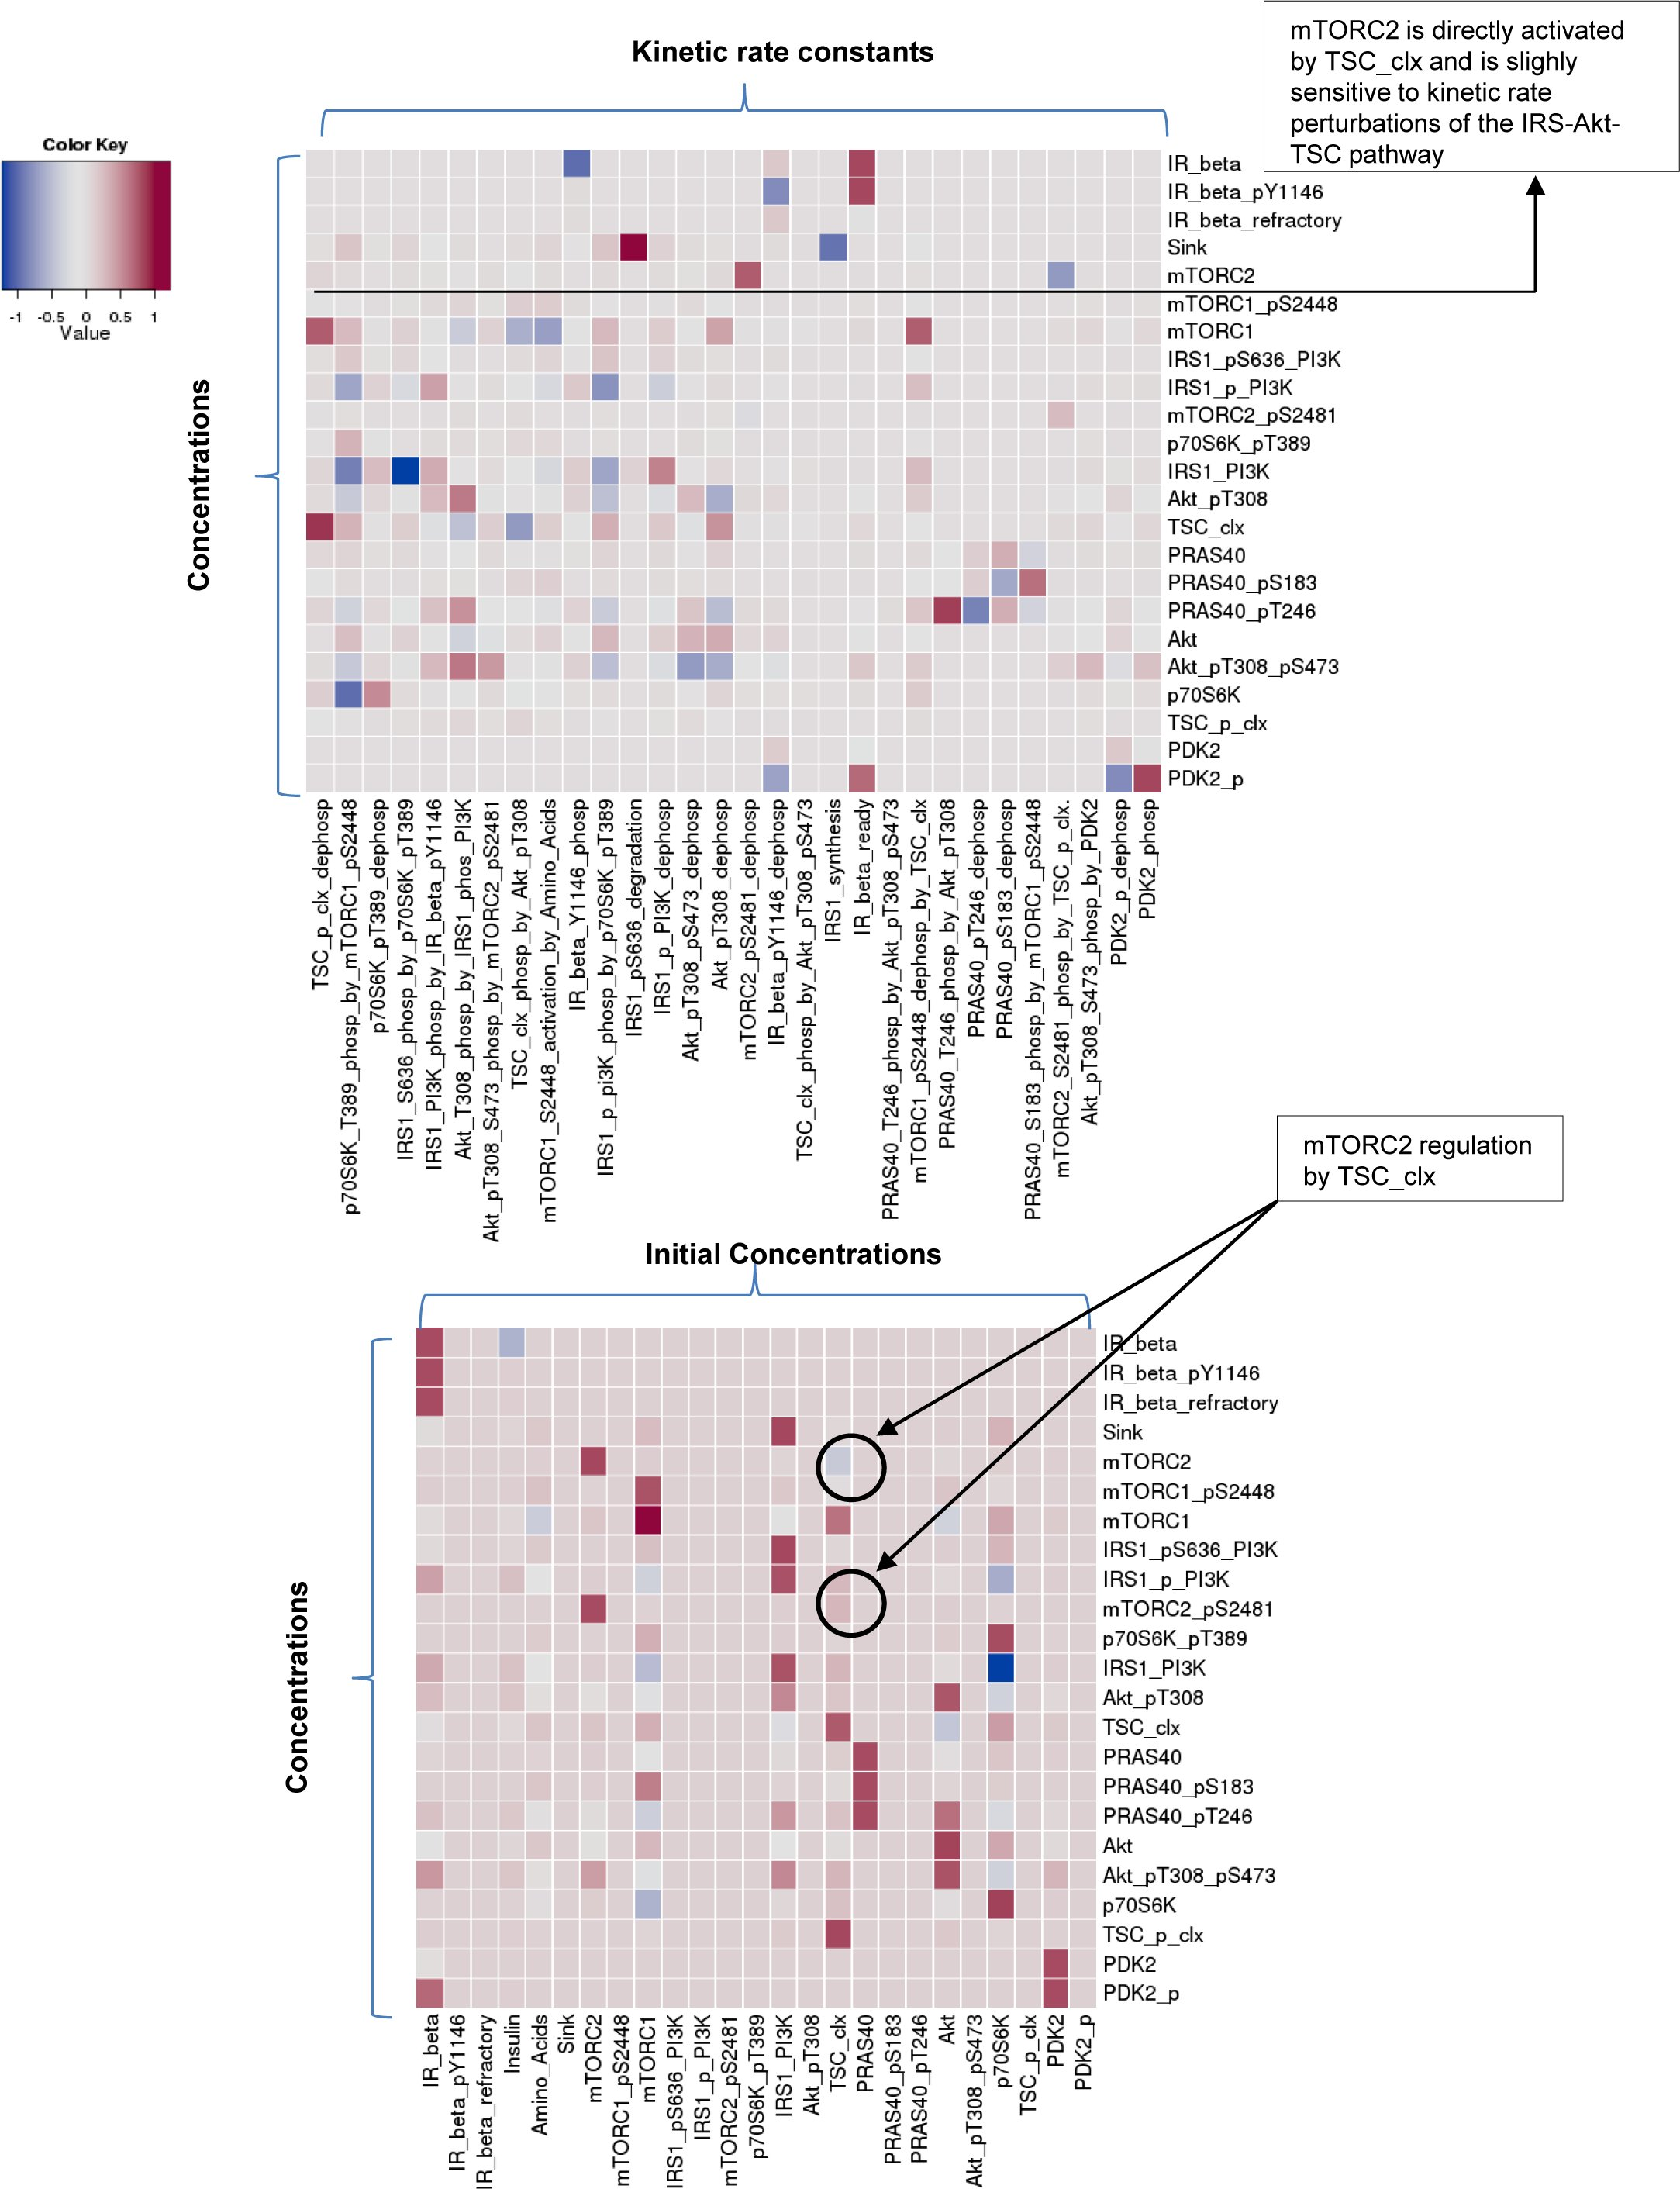
\includegraphics[width=5.10in]{2002469_supp_fig9.jpg}
		%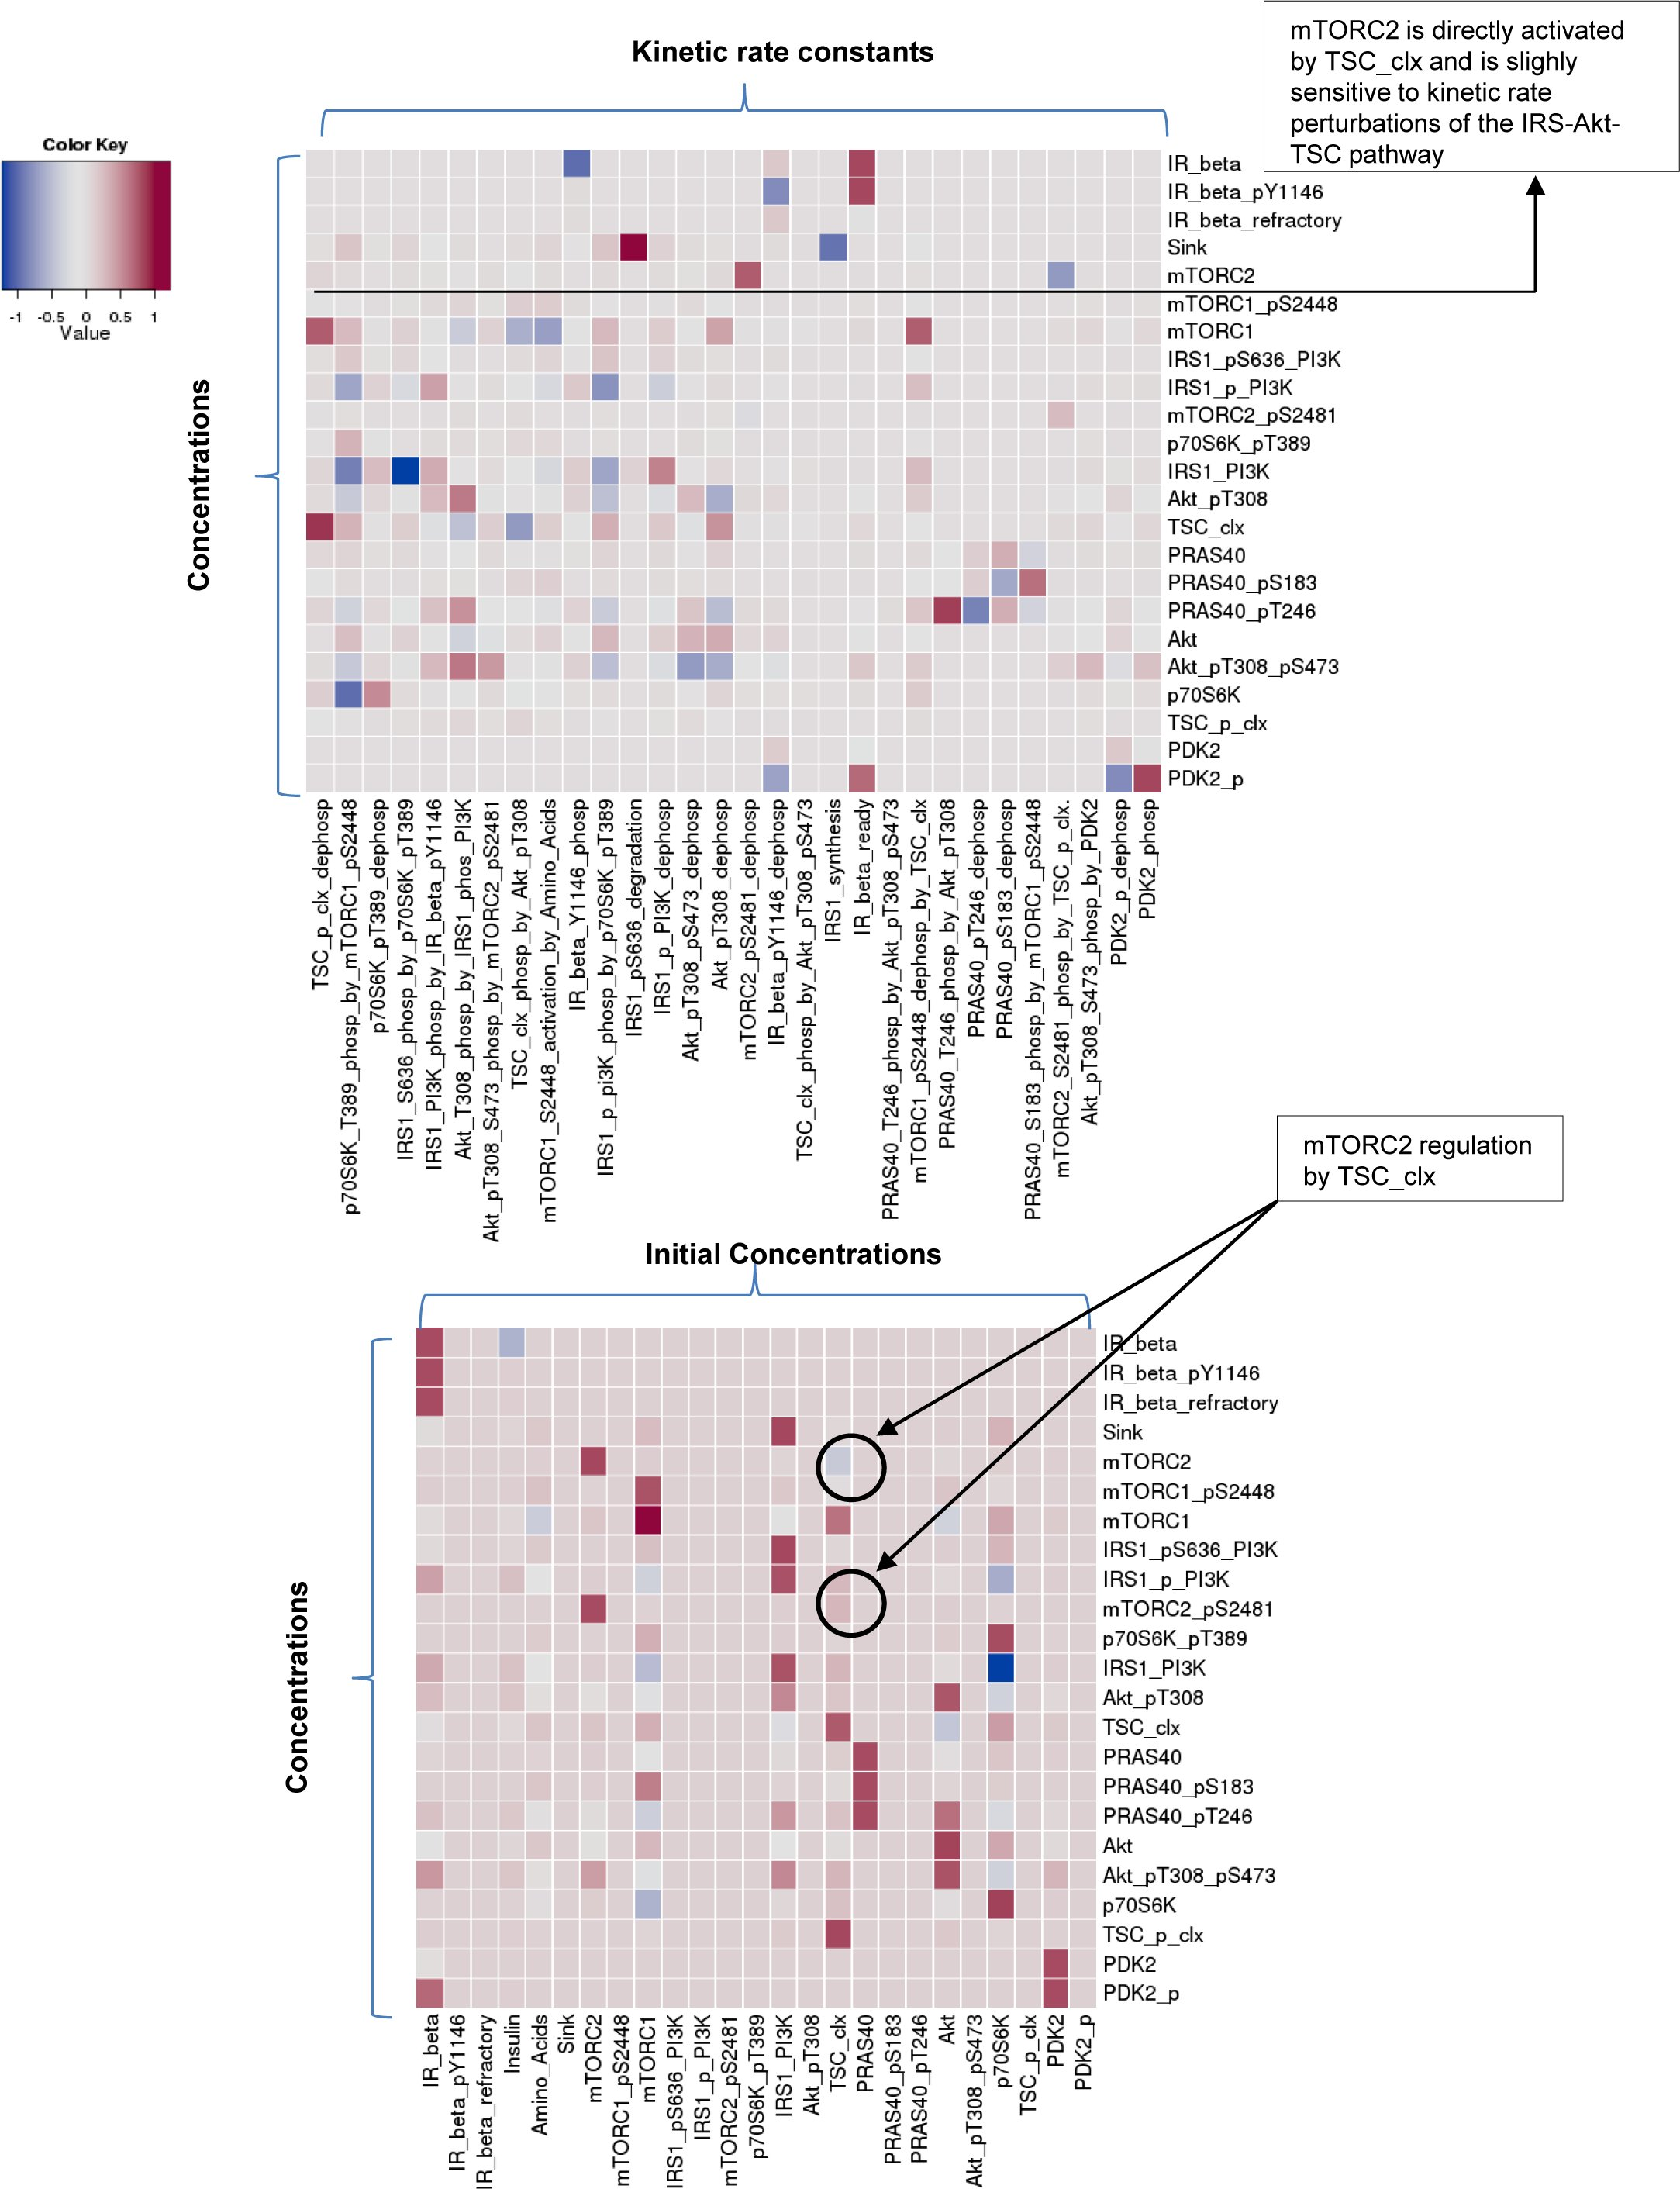
\includegraphics[scale=0.75]{2002469_supp_fig9.jpg}
		\caption[Sensitivity analysis for Hypothesis 1: TSC1/TSC2-dependent mTORC2 regulation]{Sensitivity analysis for Hypothesis 1: TSC1/TSC2-dependent mTORC2 regulation. The sensitivity analyses of the three hypotheses (see Figures \ref{fig:2002469_supp_fig11} and \ref{fig:2002469_supp_fig13}) showed a similar sensitivity analysis excluding the sensitivity for the parameters characterizing each specific hypothesis. This provided evidence that the proposed general model (common to the three hypotheses) behaved in a consistent manner following introduction of the three hypothetical models and, therefore, the three models were comparable. See Figure \ref{fig:2002469_supp_fig6} for details of the top and bottom plots.}
		\label{fig:2002469_supp_fig9}
	\end{center}
\end{figure}
\clearpage

\begin{figure}[tb]
	\begin{center}
		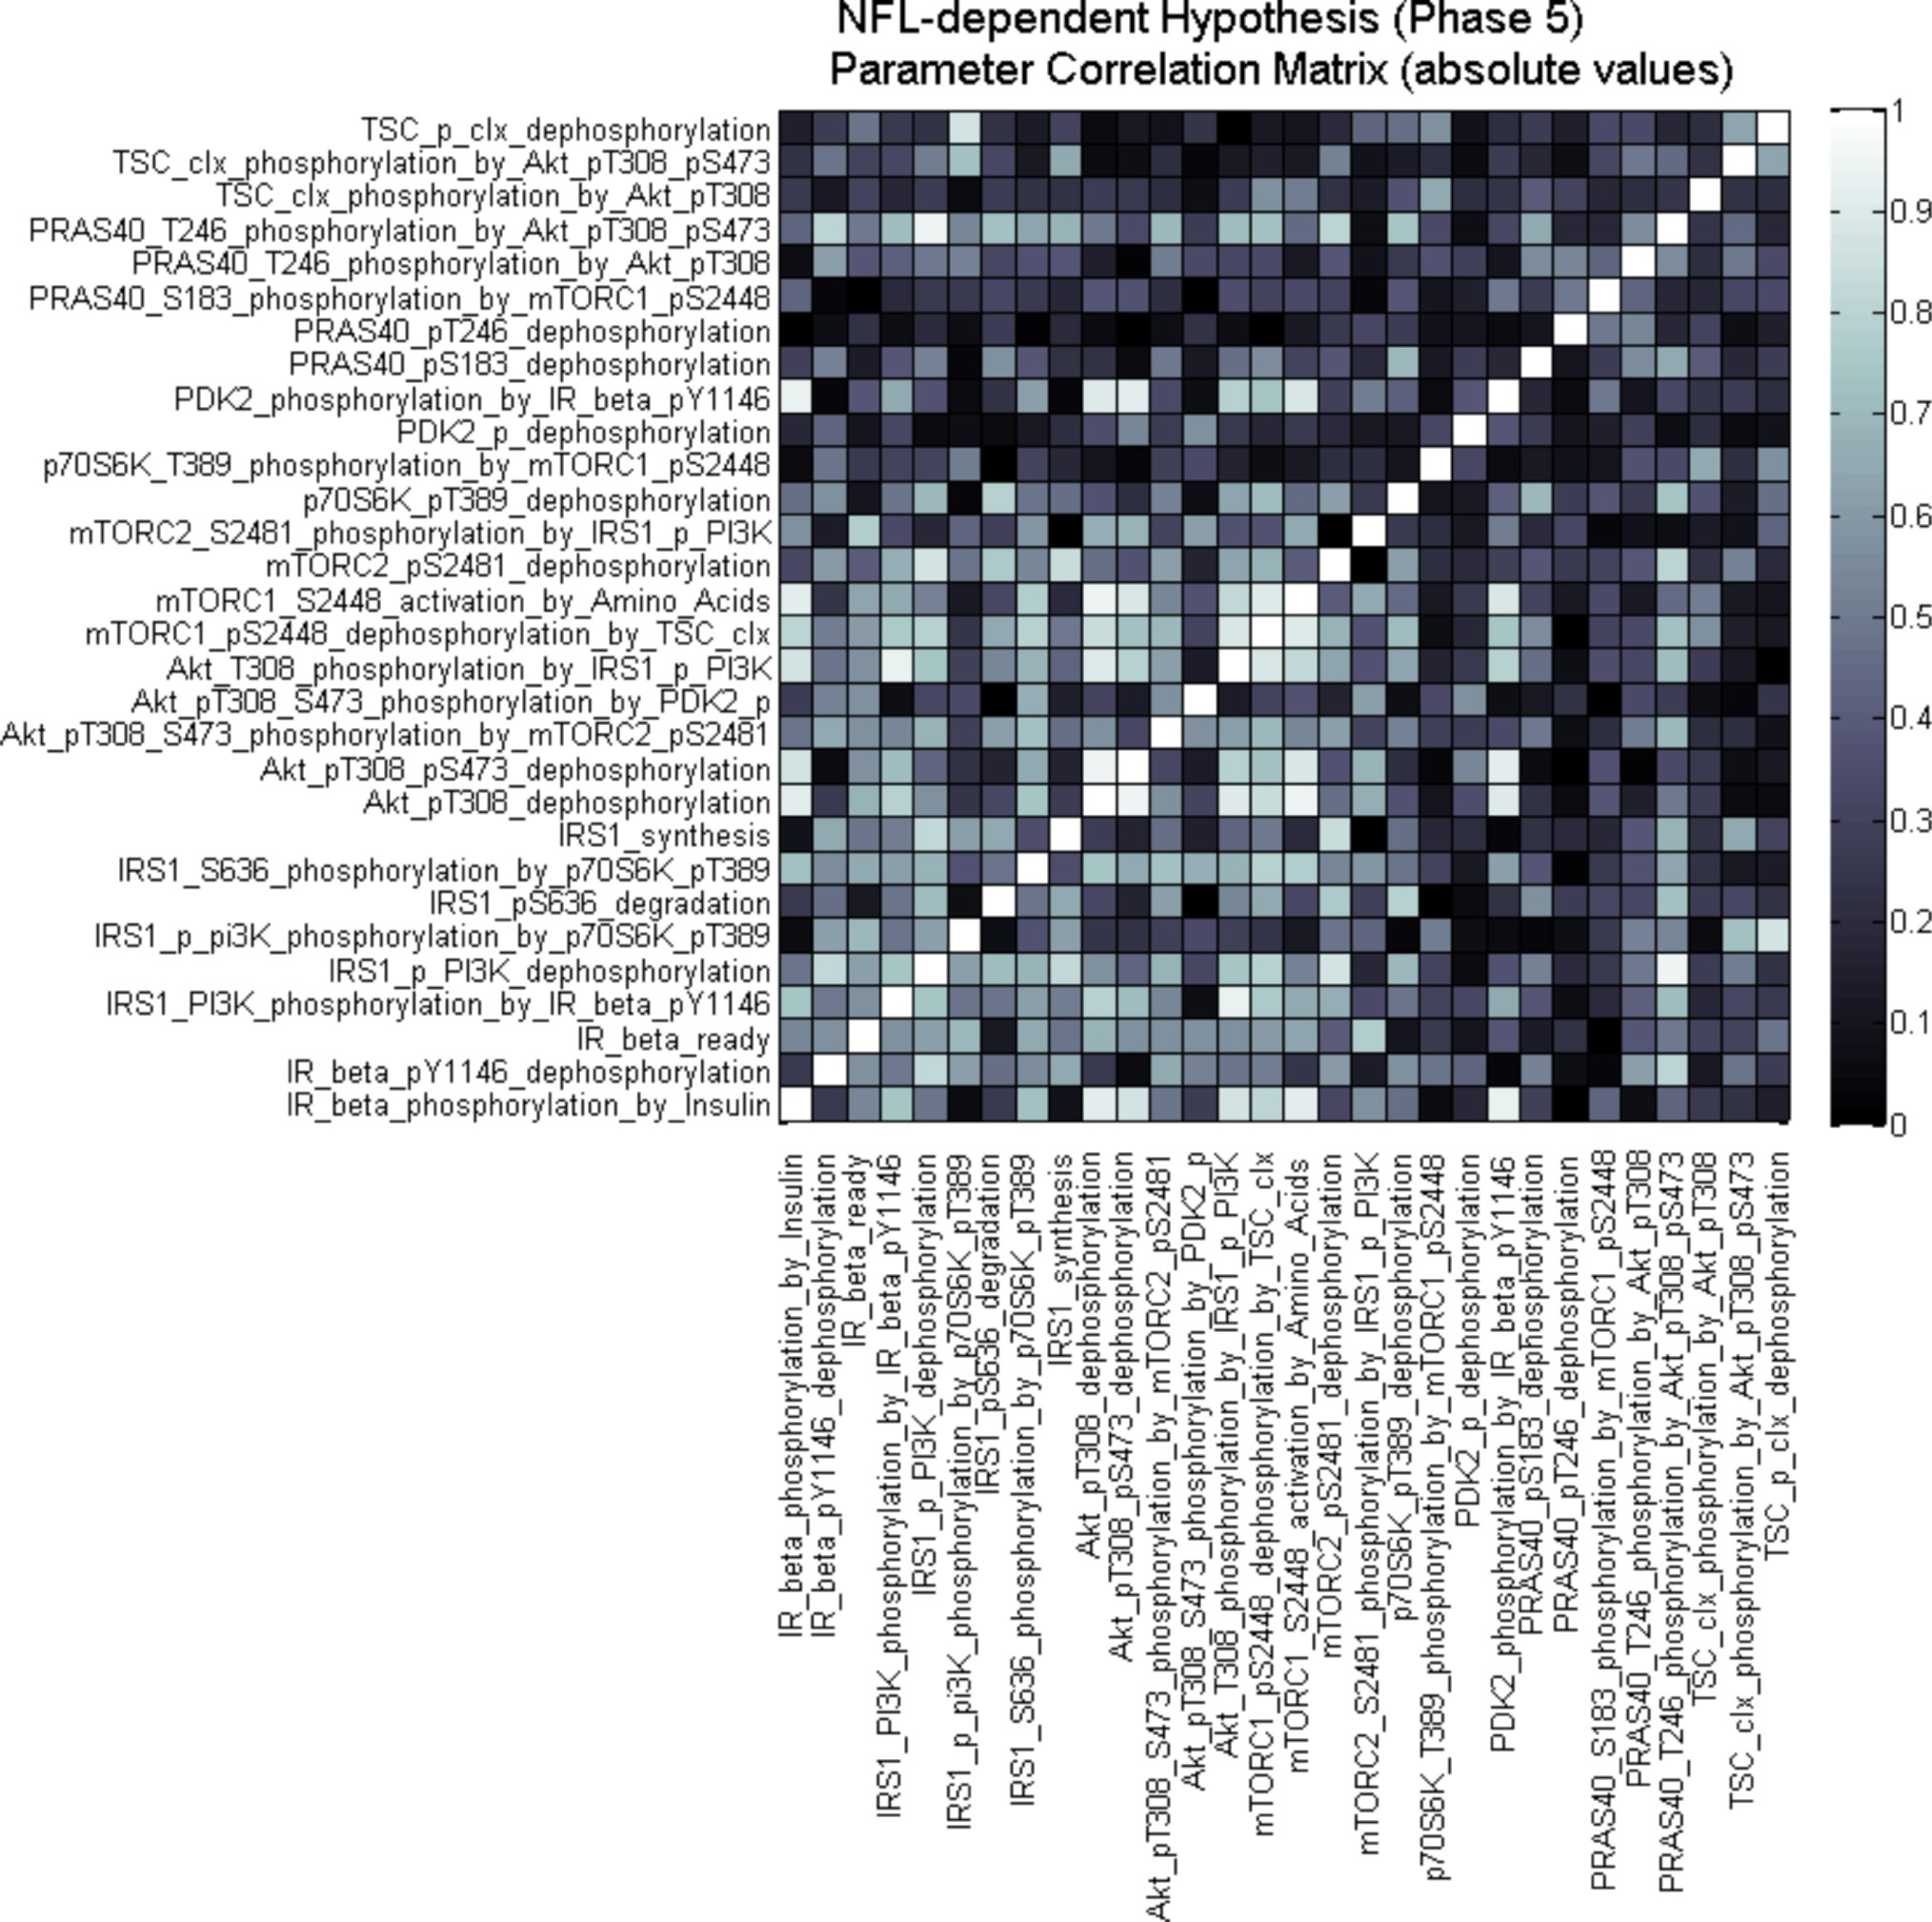
\includegraphics[scale=0.8]{2002469_supp_fig10.jpg}
		\caption[Identifiability analysis for Hypothesis 2: NFL-dependent mTORC2 regulation]{Identifiability analysis for Hypothesis 2: NFL-dependent mTORC2 regulation. Parameter correlation matrix for NFL-dependent hypothesis is shown. See Figure \ref{fig:2002469_supp_fig5} for details.}
		\label{fig:2002469_supp_fig10}
	\end{center}
\end{figure}
\clearpage

\begin{figure}[tb]
	\begin{center}
		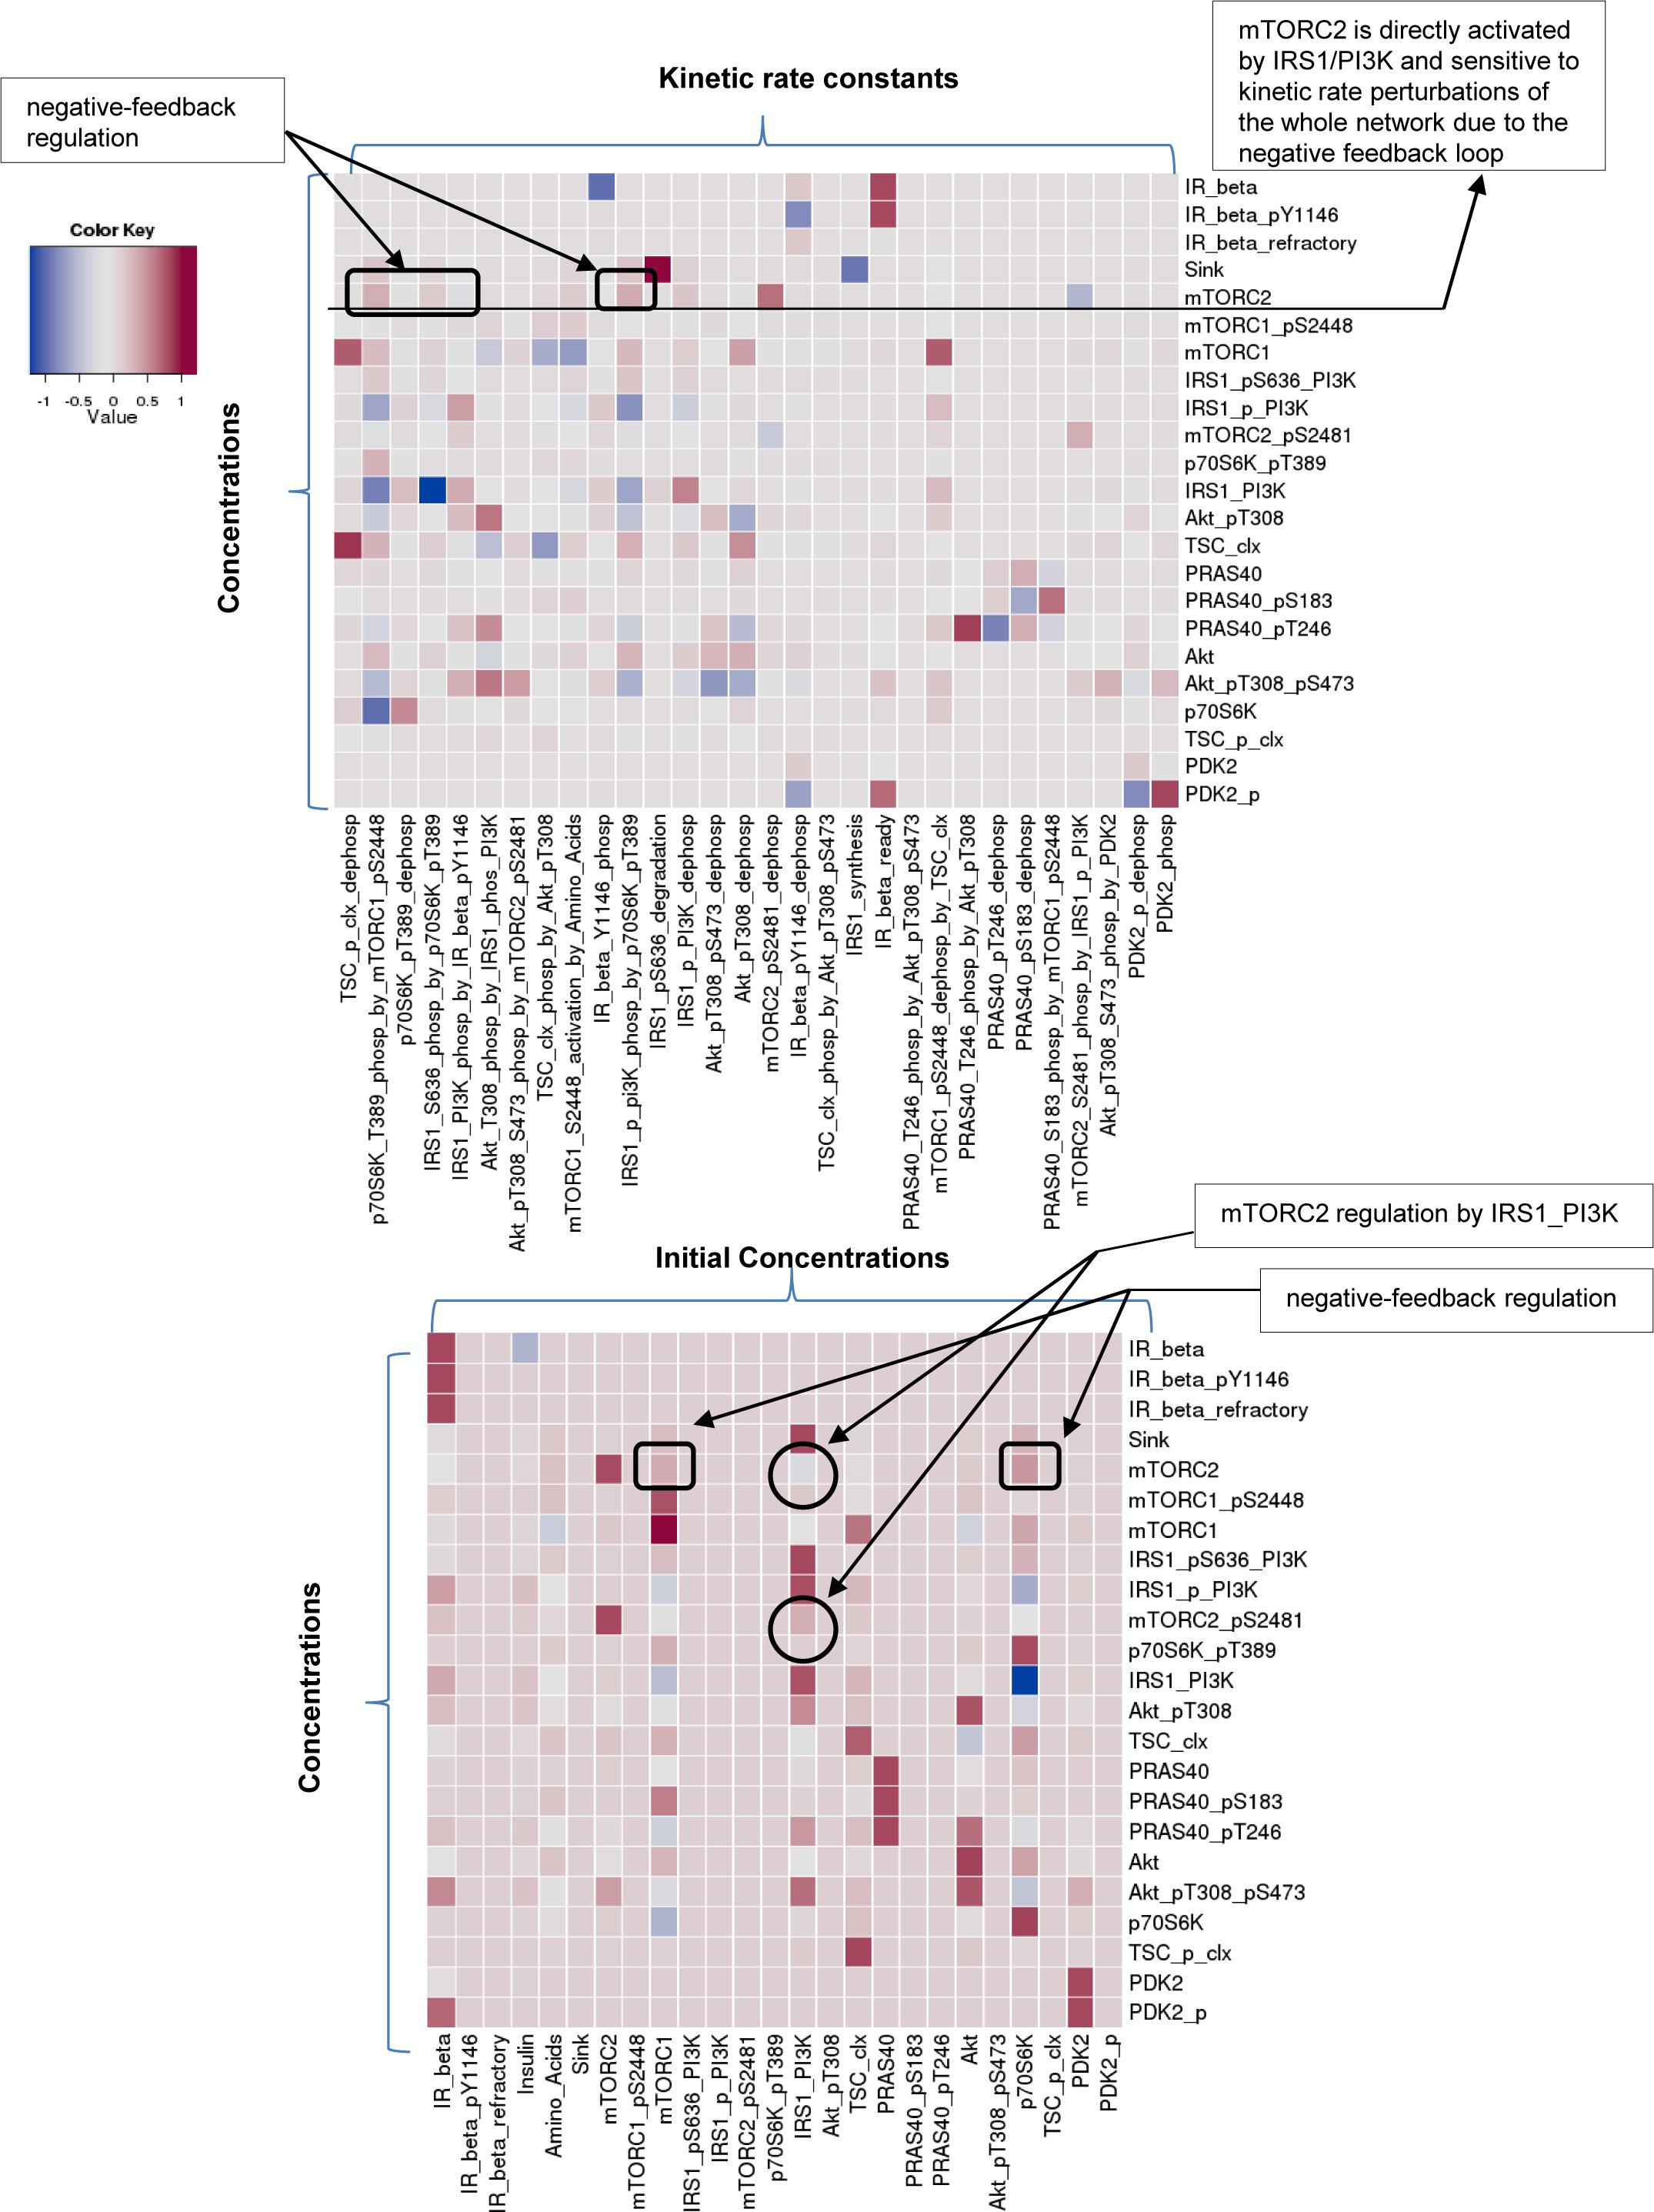
\includegraphics[scale=0.75]{2002469_supp_fig11.jpg}
		\caption[Sensitivity analysis for Hypothesis 2: NFL-dependent mTORC2 regulation]{Sensitivity analysis for Hypothesis 2: NFL-dependent mTORC2 regulation. Sensitivity analysis for the initial concentrations and the kinetic rates parameters for the NFL-dependent hypothesis is shown.  See Figure \ref{fig:2002469_supp_fig6} for details of the top and bottom plots.}
		\label{fig:2002469_supp_fig11}
	\end{center}
\end{figure}
\clearpage

\begin{figure}[tb]
	\begin{center}
		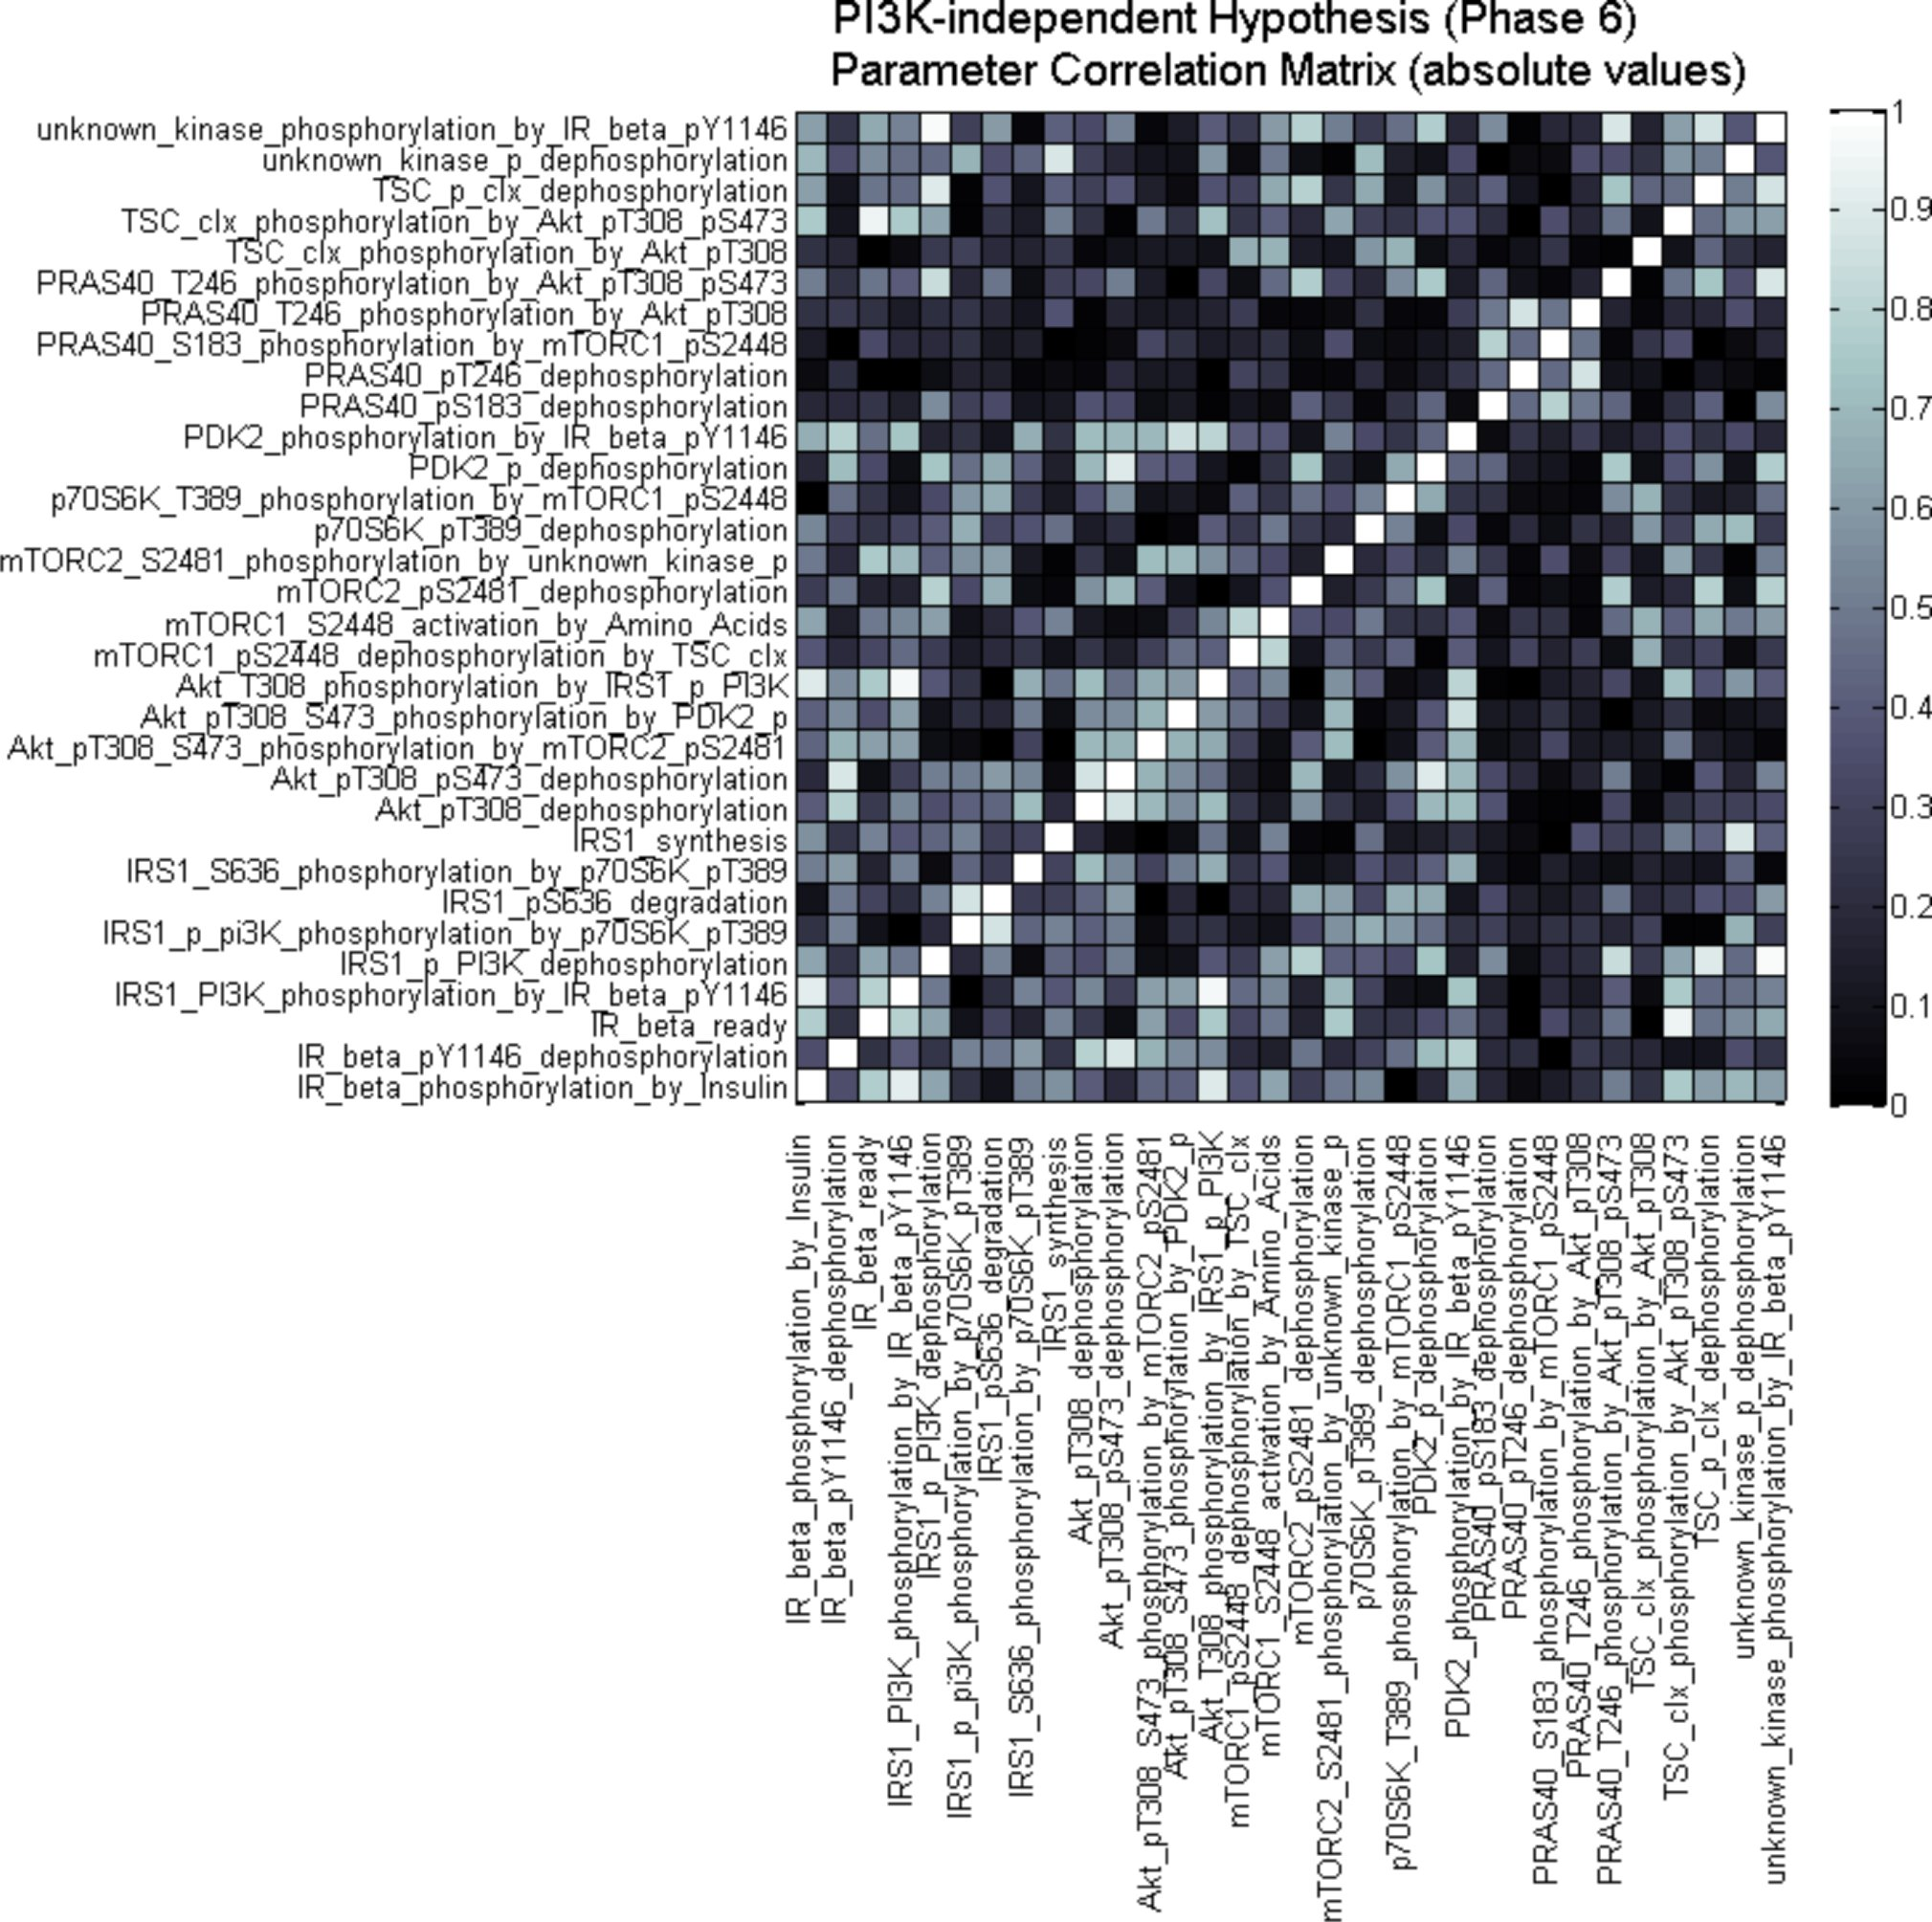
\includegraphics[scale=0.8]{2002469_supp_fig12.jpg}
		\caption[Identifiability analysis for Hypothesis 3: PI3K-independent mTORC2 regulation]{Identifiability analysis for Hypothesis 3: PI3K-independent mTORC2 regulation. Parameter correlation matrix for PI3K-independent hypothesis is shown. See Figure \ref{fig:2002469_supp_fig5} for details.}
		\label{fig:2002469_supp_fig12}
	\end{center}
\end{figure}
\clearpage

\begin{figure}[tb]
	\begin{center}
		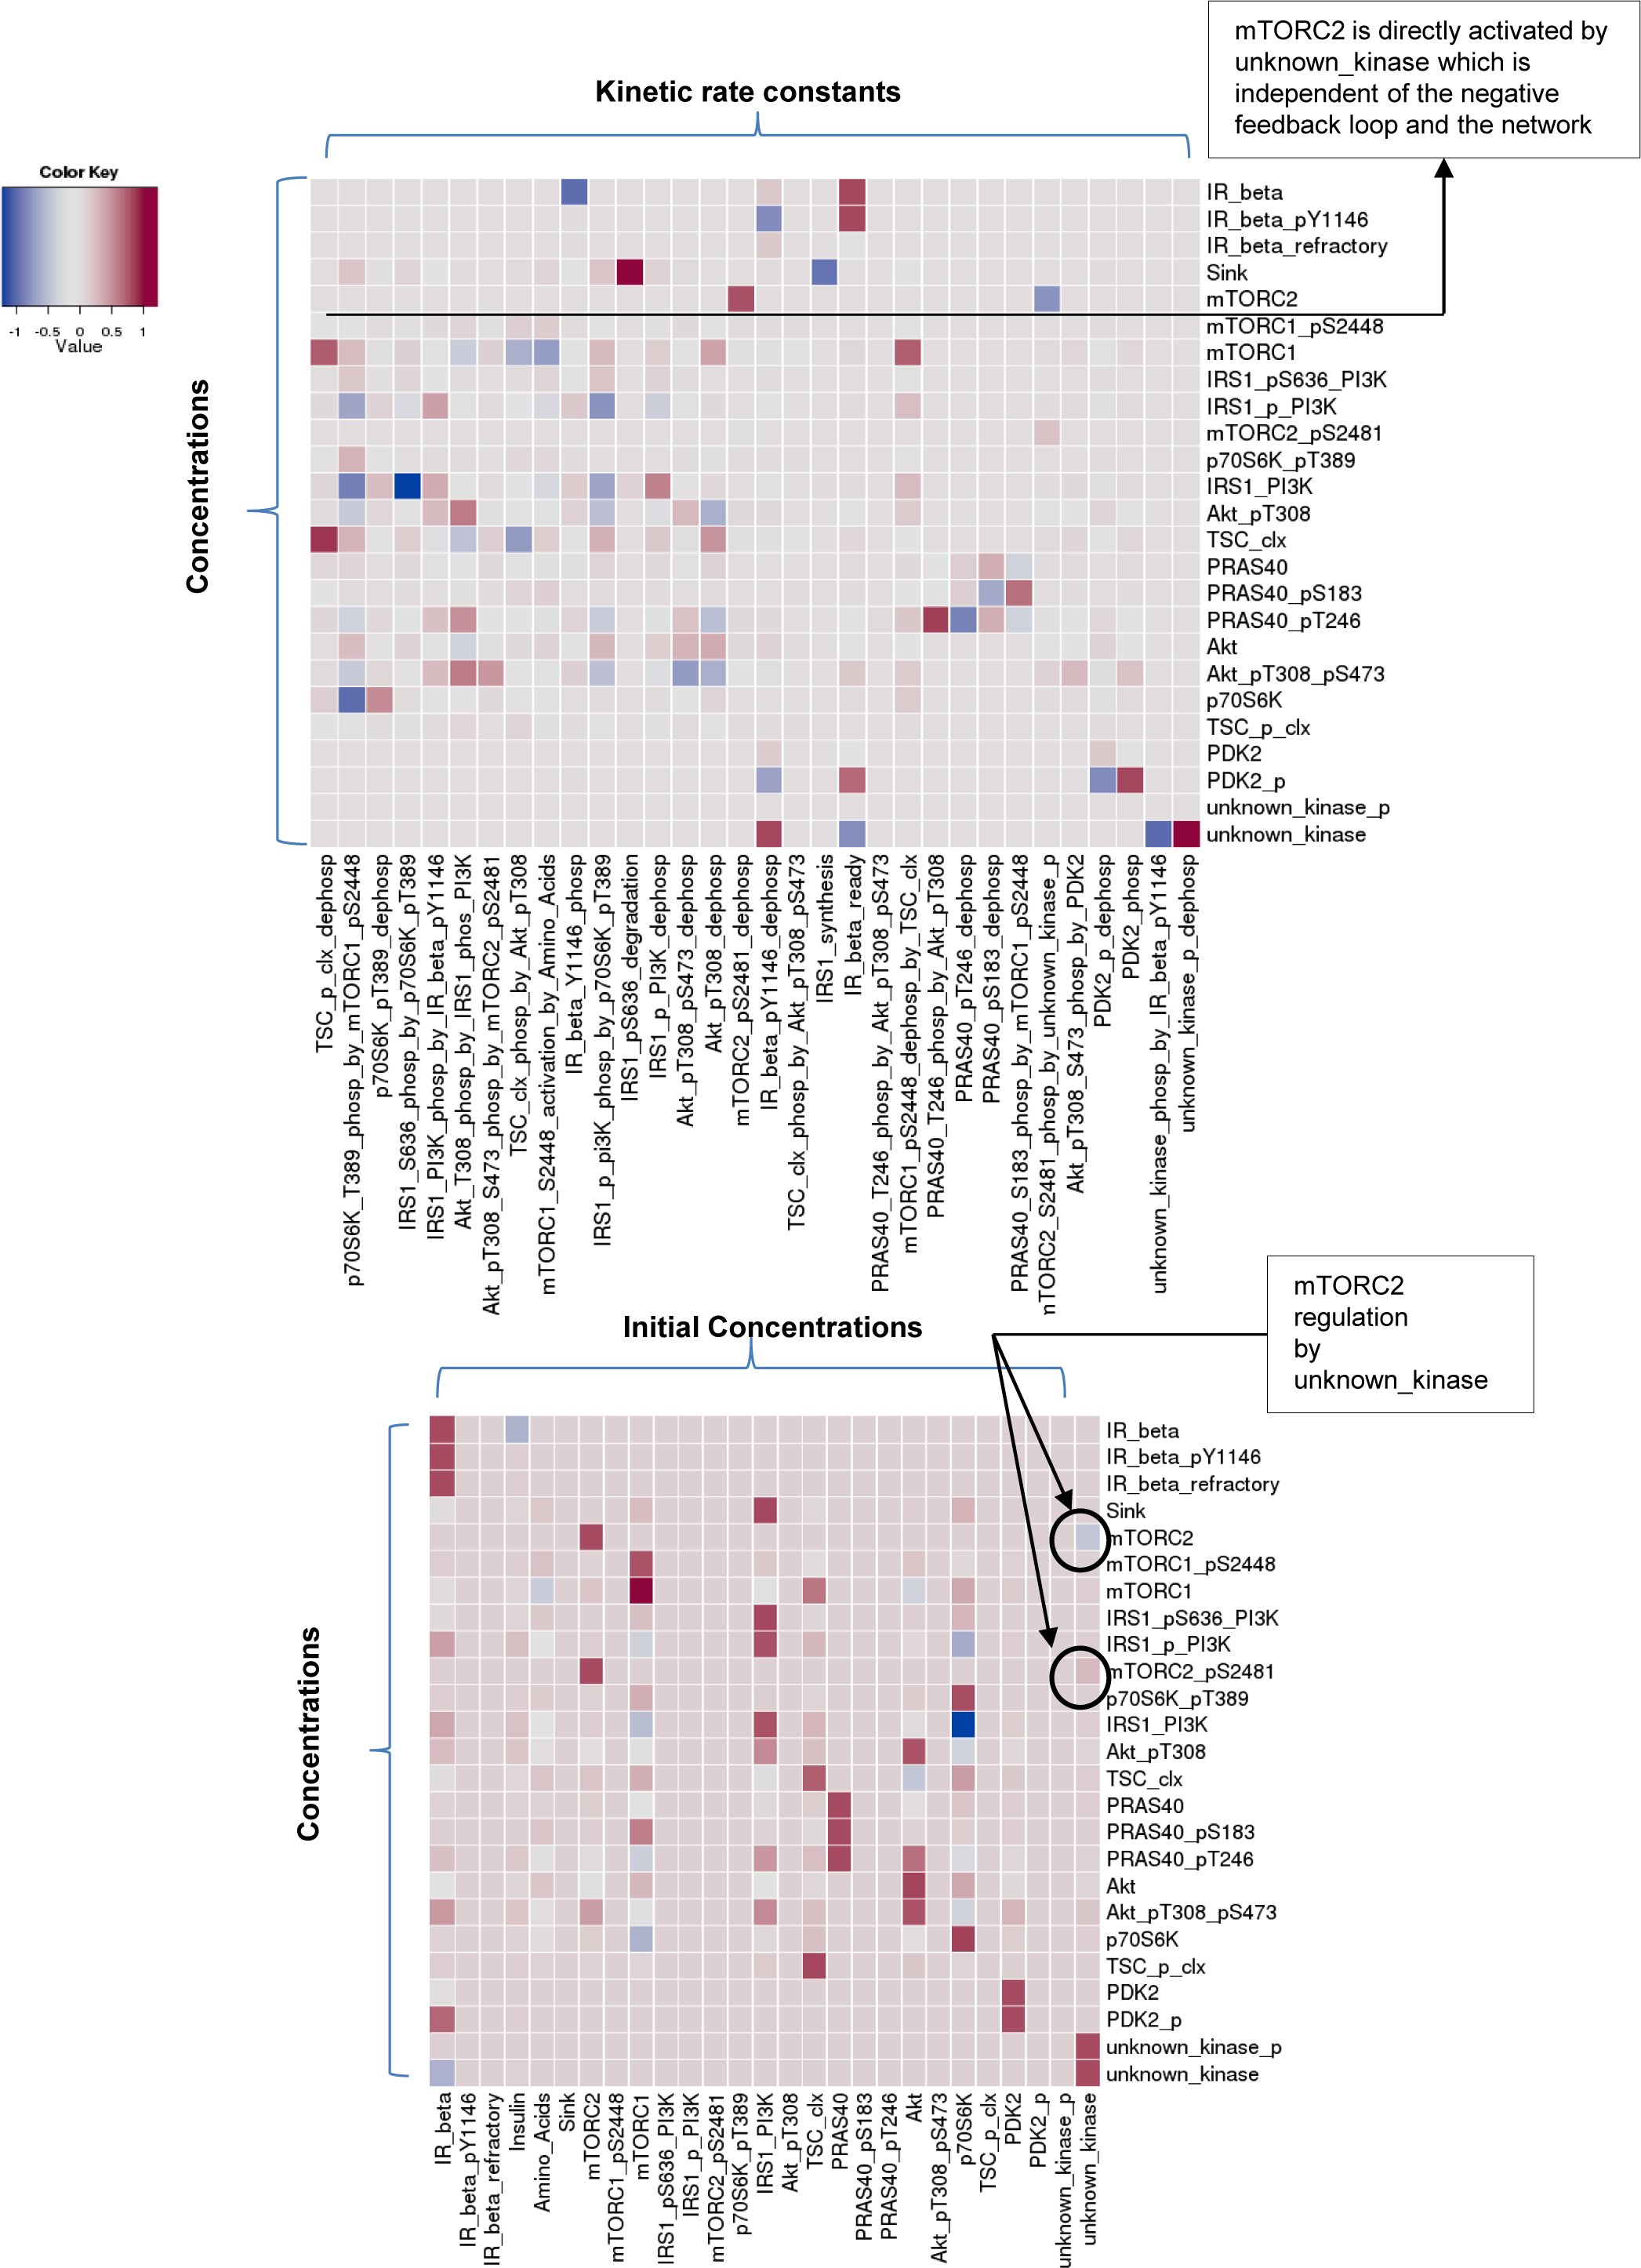
\includegraphics[scale=0.75]{2002469_supp_fig13.jpg}
		\caption[Sensitivity analysis for Hypothesis 3: PI3K-independent mTORC2 regulation]{Sensitivity analysis for Hypothesis 3: PI3K-independent mTORC2 regulation. Sensitivity analysis for the initial concentrations and the kinetic rates parameters for the PI3K-independent hypothesis is shown. See Figure \ref{fig:2002469_supp_fig6} for details of the top and bottom plots.}
		\label{fig:2002469_supp_fig13}
	\end{center}
\end{figure}
\clearpage

\begin{figure}[tb]
	\begin{center}
		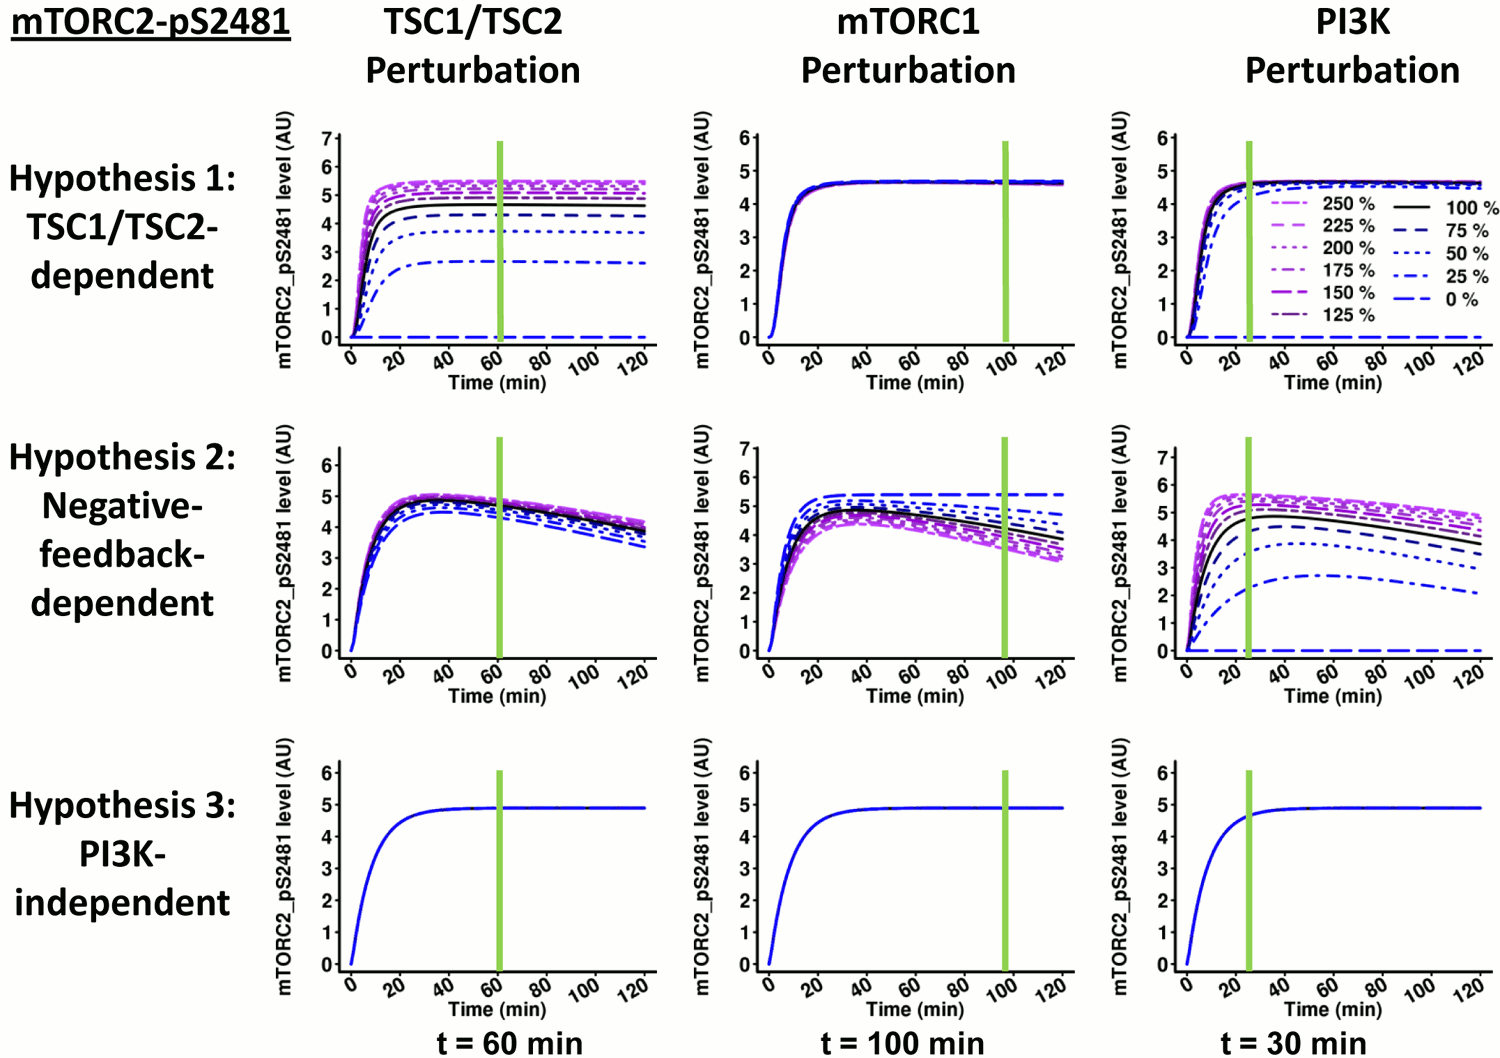
\includegraphics[scale=1.1]{2002469_fig5A.png}
		\caption[Simulations of network perturbations at several levels and differential dynamical network responses for the three different hypotheses (mTOR-pS2481 readout)]{Simulations of network perturbations at several levels and differential dynamical network responses for the three different hypotheses (mTOR-pS2481 readout). Simulated mTOR-pS2481 response upon amino acids/insulin induction in systems with the indicated perturbations: TSC1/TSC2 (experimental equivalent: gradual TSC2 knockdown), mTORC1 (experimental equivalent: gradual Raptor knockdown), and PI3K (experimental equivalent: gradual PI3K inhibition with Wortmannin) for Hypothesis 1, 2, and 3. The time points that were experimentally tested are indicated with green lines.}
		\label{fig:2002469_fig5A}
	\end{center}
\end{figure}

\clearpage
\begin{figure}[tb]
	\begin{center}
		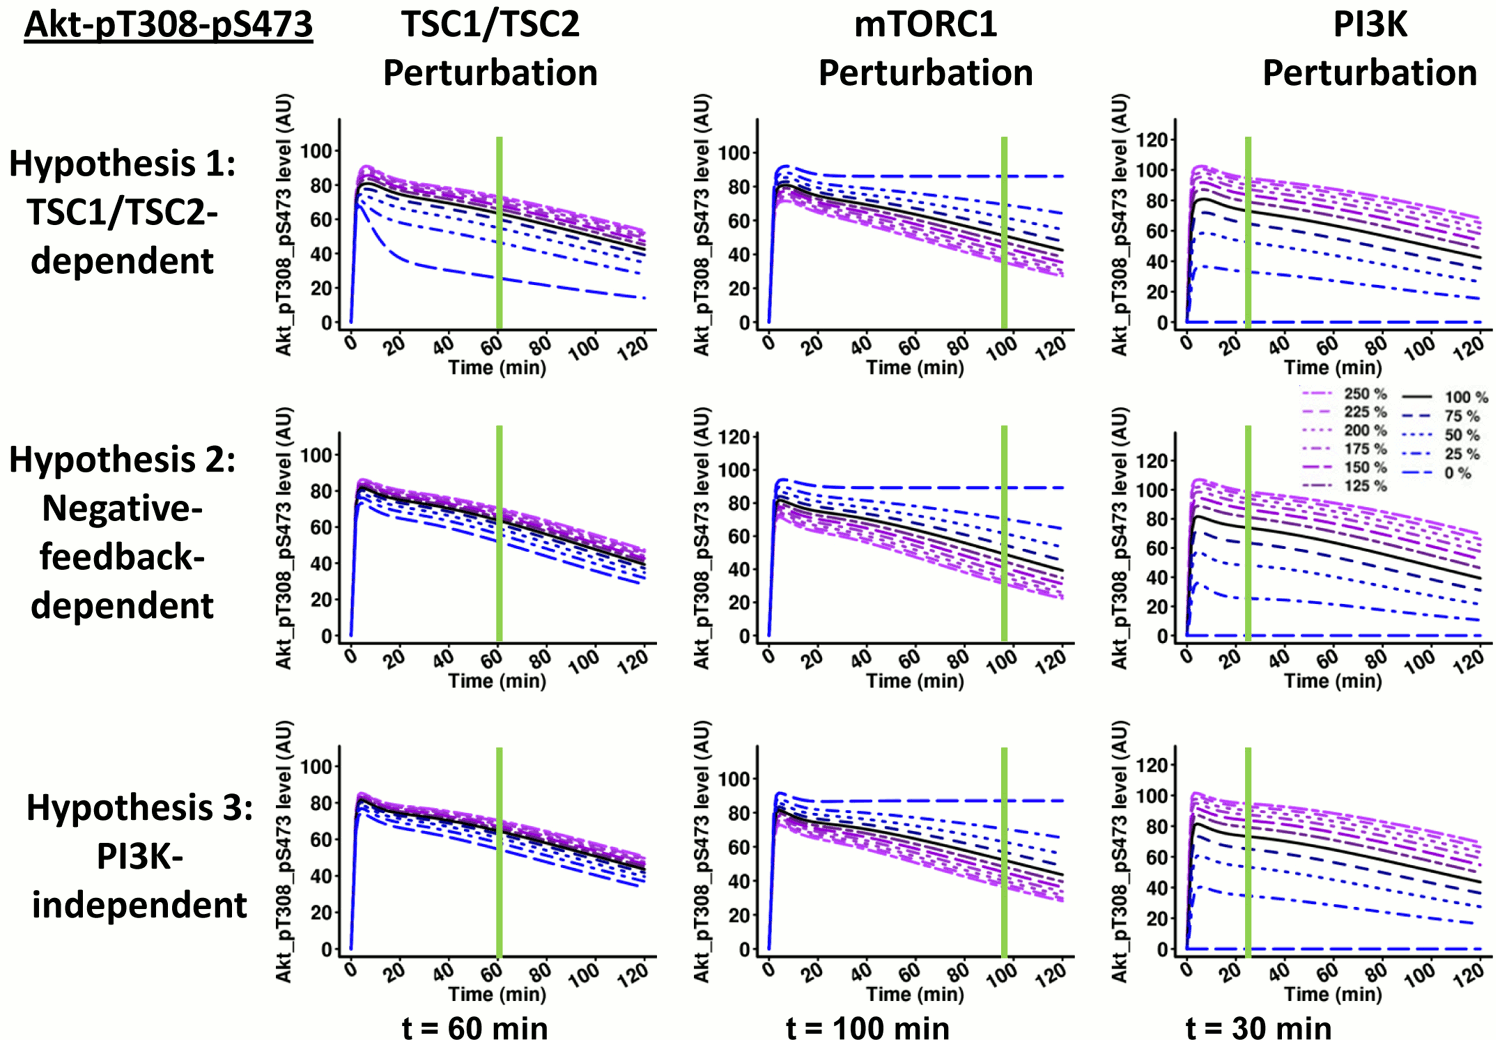
\includegraphics[scale=1.1]{2002469_fig5B.png}
		\caption[Simulations of network perturbations at several levels and differential dynamical network responses for the three different hypotheses (Akt-pS473 readout)]{Simulations of network perturbations at several levels and differential dynamical network responses for the three different hypotheses (Akt-pS473 readout). Simulated Akt-pT308-pS473 response for each of the three hypotheses upon amino acids/insulin induction in systems with perturbations of TSC1/TSC2, mTORC1, and PI3K. The time points that were experimentally tested are indicated with green lines.}
		\label{fig:2002469_fig5B}
	\end{center}
\end{figure}
\clearpage

\begin{figure}[tb]
	\begin{center}
		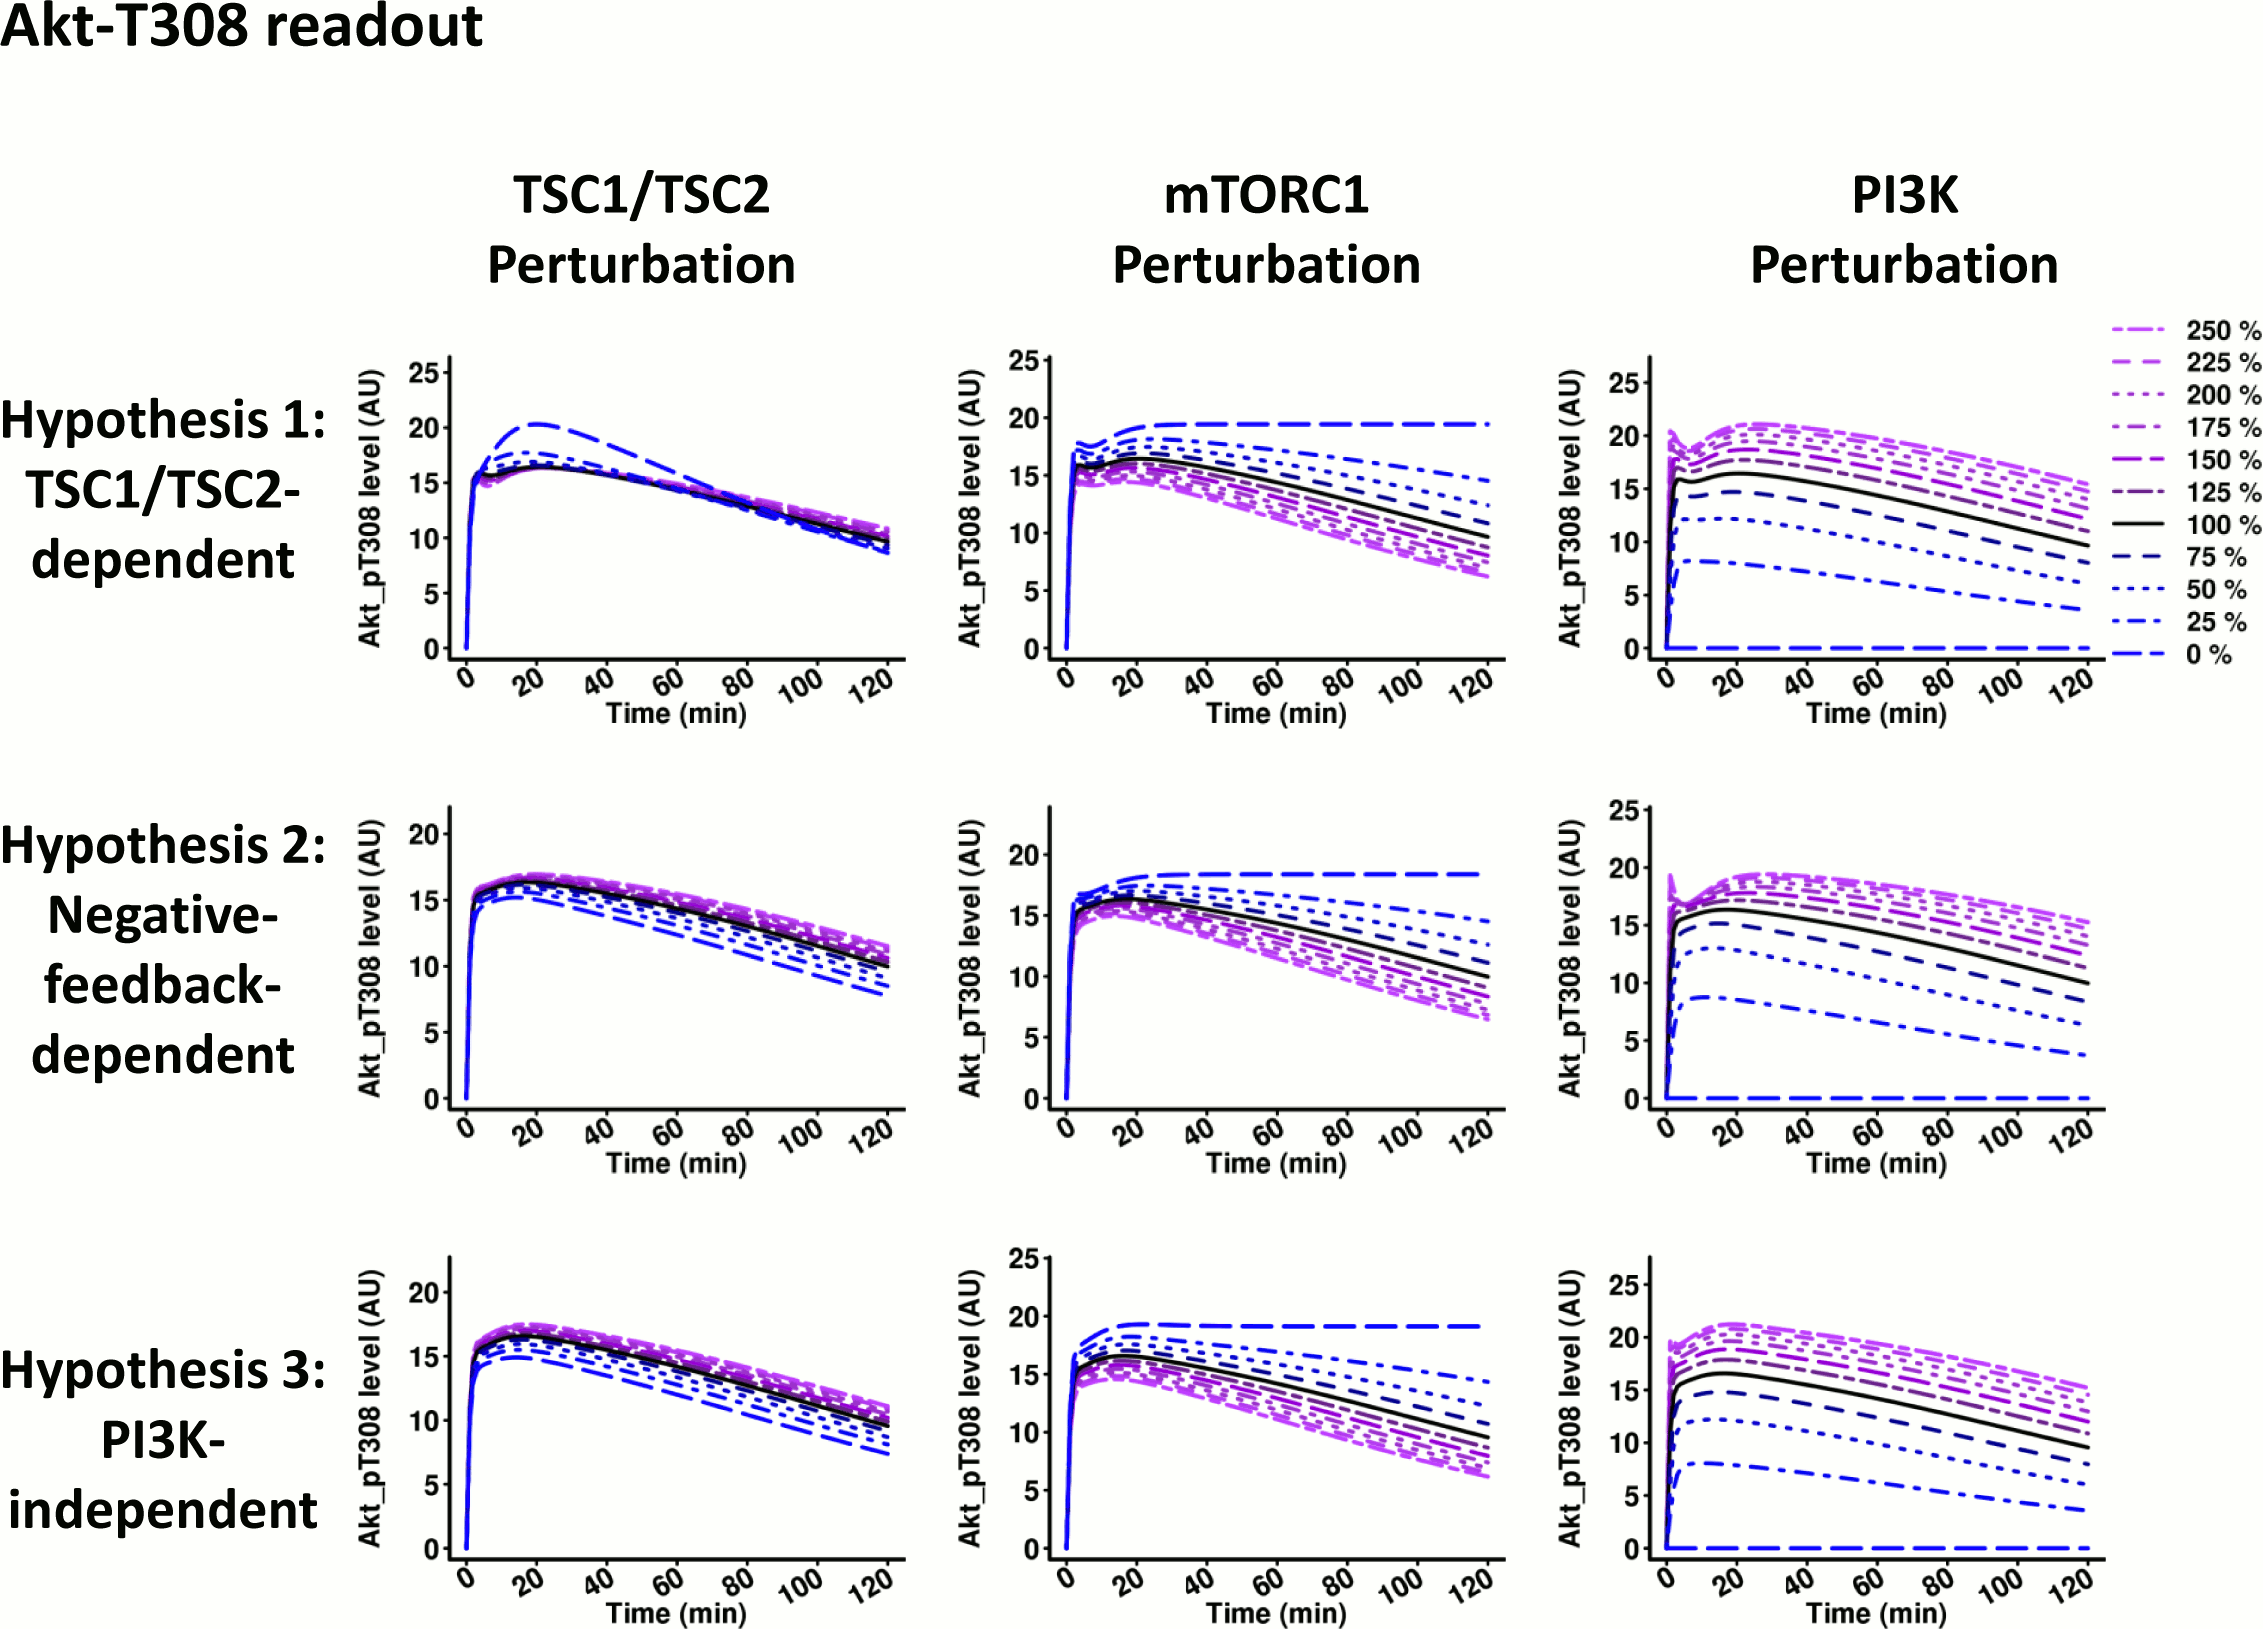
\includegraphics[scale=0.74]{2002469_supp_fig14.png}
		\caption[The influence of perturbations of TSC1/TSC2, mTORC1, or PI3K on the phosphorylation of Akt-T308 for the three hypotheses]{The influence of perturbations of TSC1/TSC2, mTORC1, or PI3K on the phosphorylation of Akt-T308 for the three hypotheses. The three hypotheses did not show any difference in the dynamics of Akt-T308 phosphorylation when varying the amounts of PI3K and mTORC1. A small difference was observed for TSC1/TSC2 perturbation where the TSC1/TSC2-dependent hypothesis showed a slight increase in Akt-T308 phosphorylation when TSC1/TSC2 activity was reduced. In the TSC1/TSC2-dependent hypothesis, the mTORC2 activity is reduced when the amount of TSC1/TSC2 is reduced.}
		\label{fig:2002469_supp_fig14}
	\end{center}
\end{figure}
\clearpage

\begin{figure}[tb]
	\begin{center}
		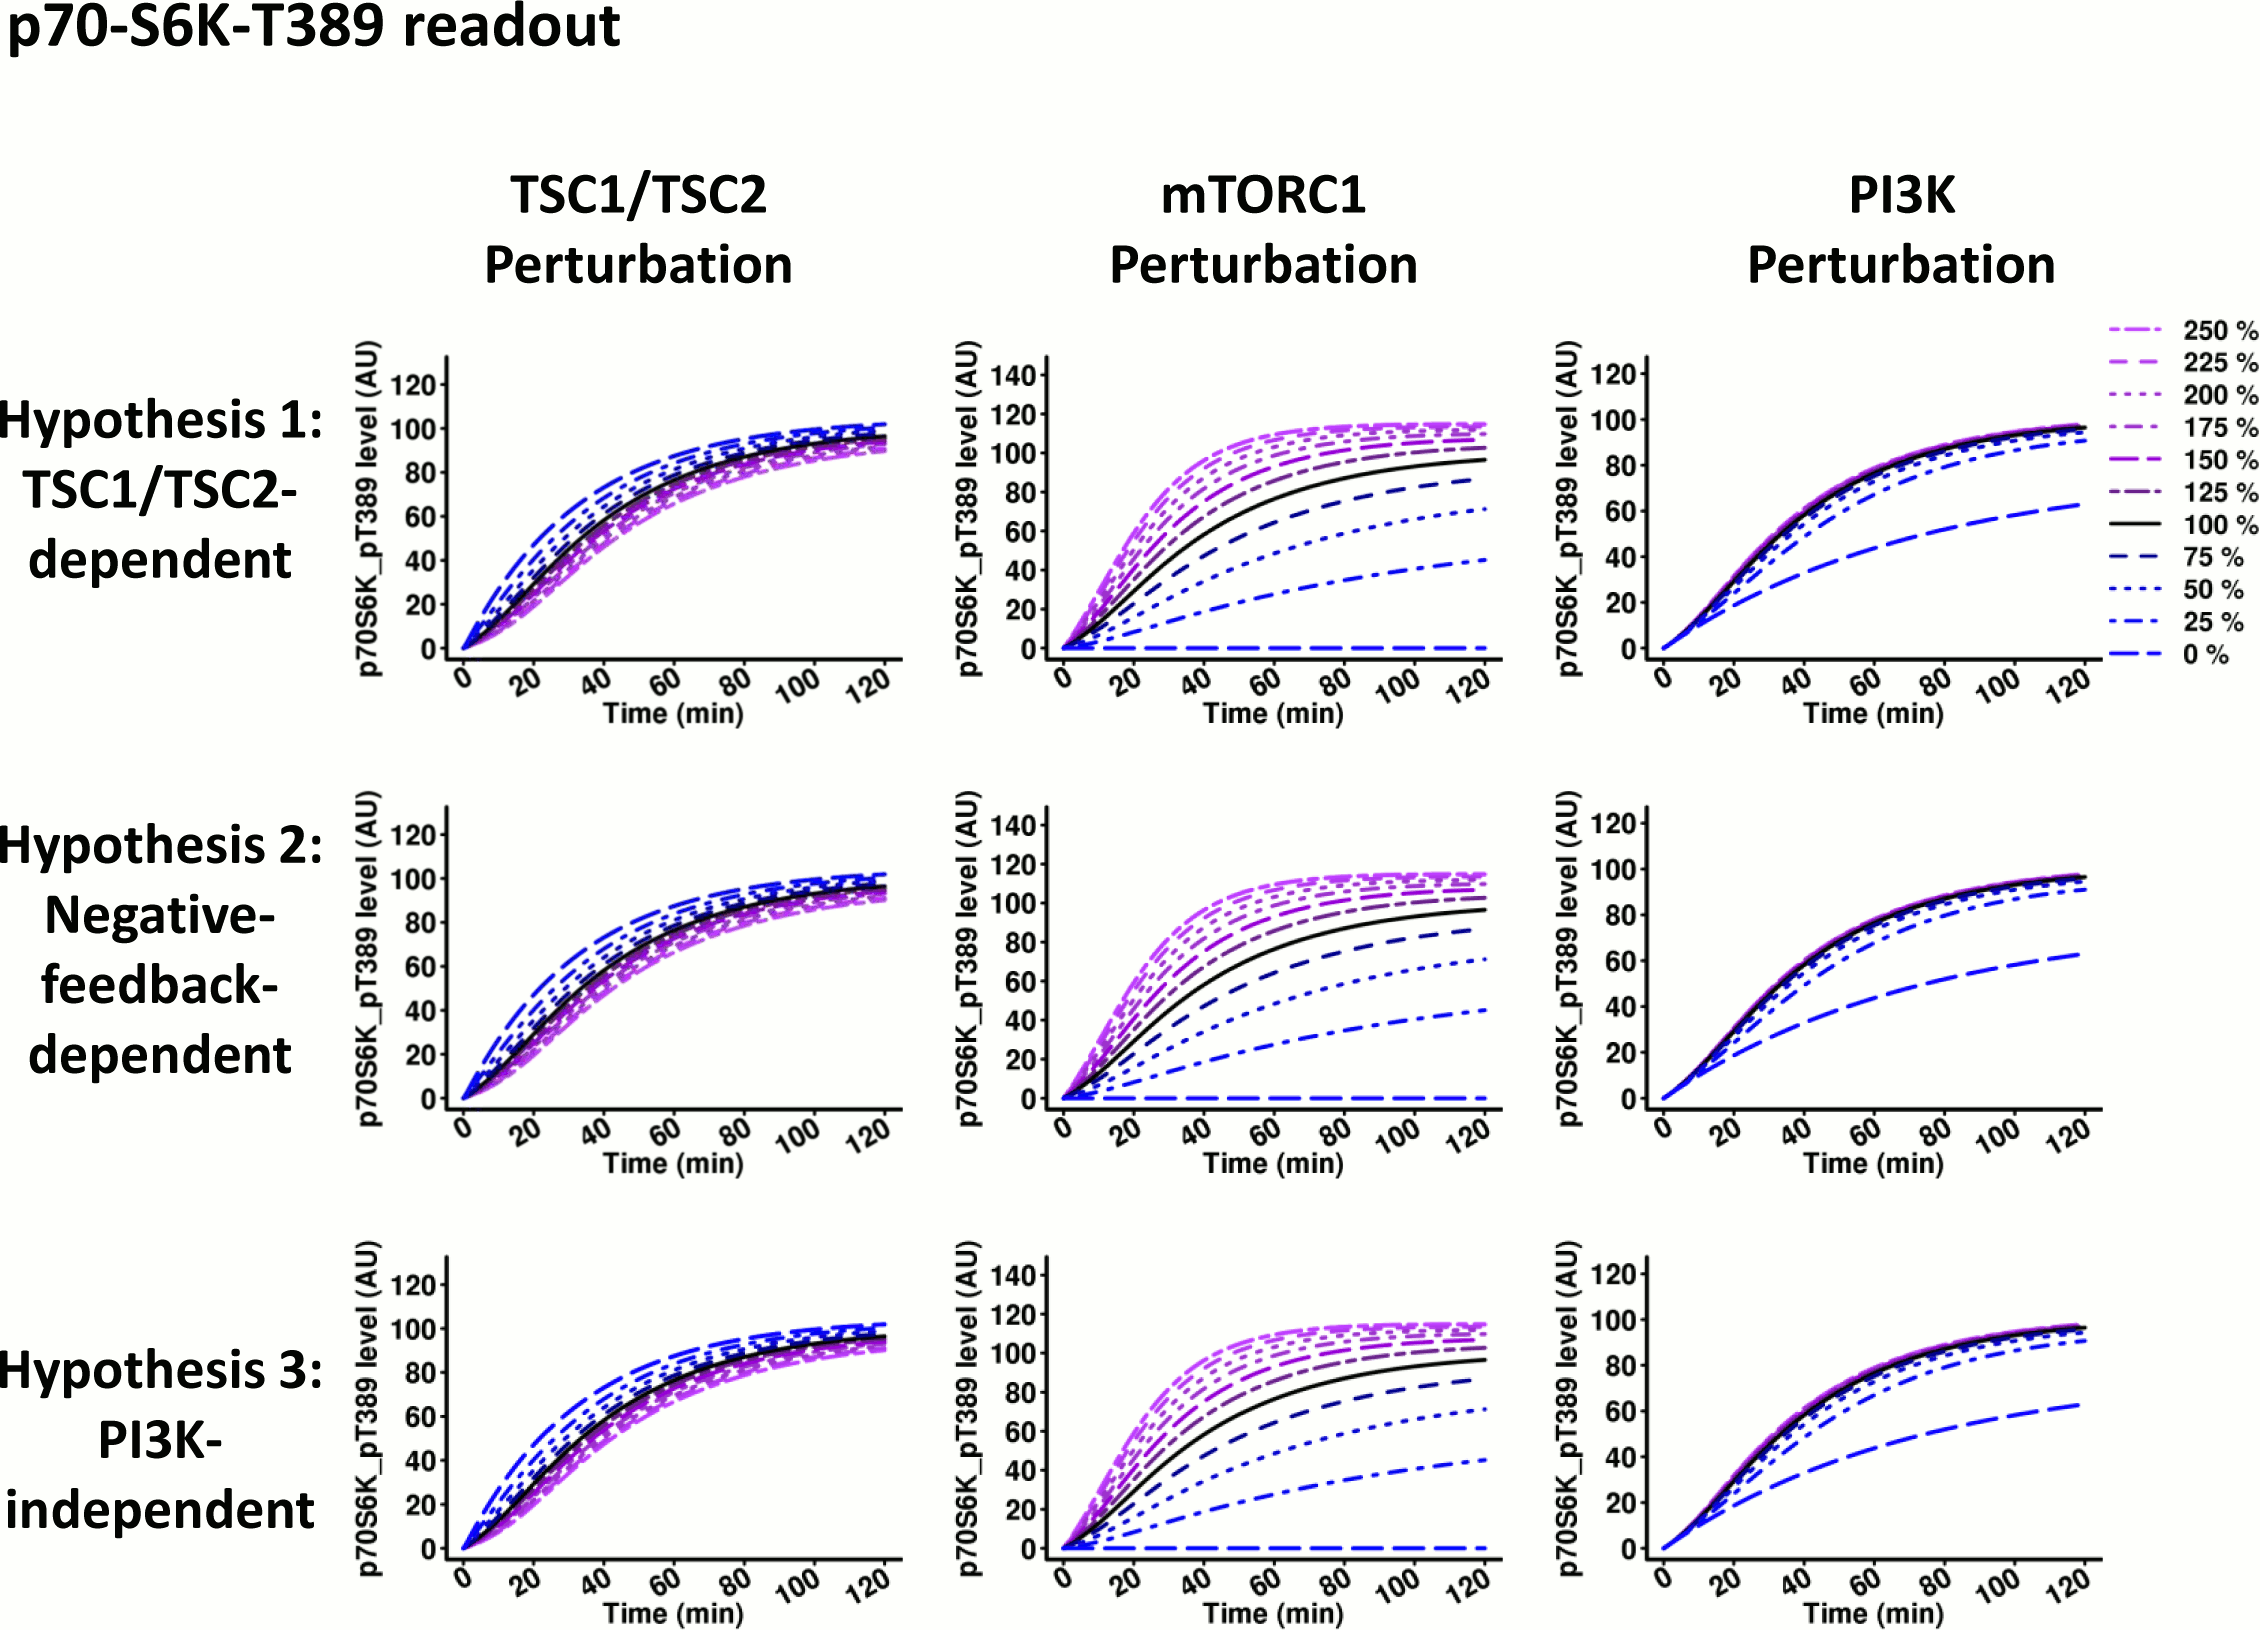
\includegraphics[scale=0.74]{2002469_supp_fig15.png}
		\caption[The influence of perturbations of TSC1/TSC2, mTORC1, or PI3K on the phosphorylation of p70-S6K-T389 for the three hypotheses]{The influence of perturbations of TSC1/TSC2, mTORC1, or PI3K on the phosphorylation of p70-S6K-T389 for the three hypotheses. The effect of each perturbation on the networks representing each hypothesis for the phosphorylation of p70-S6K-T389, which is a readout for mTORC1 activity, is shown.}
		\label{fig:2002469_supp_fig15}
	\end{center}
\end{figure}
\clearpage

\begin{figure}[tb]
	\begin{center}
		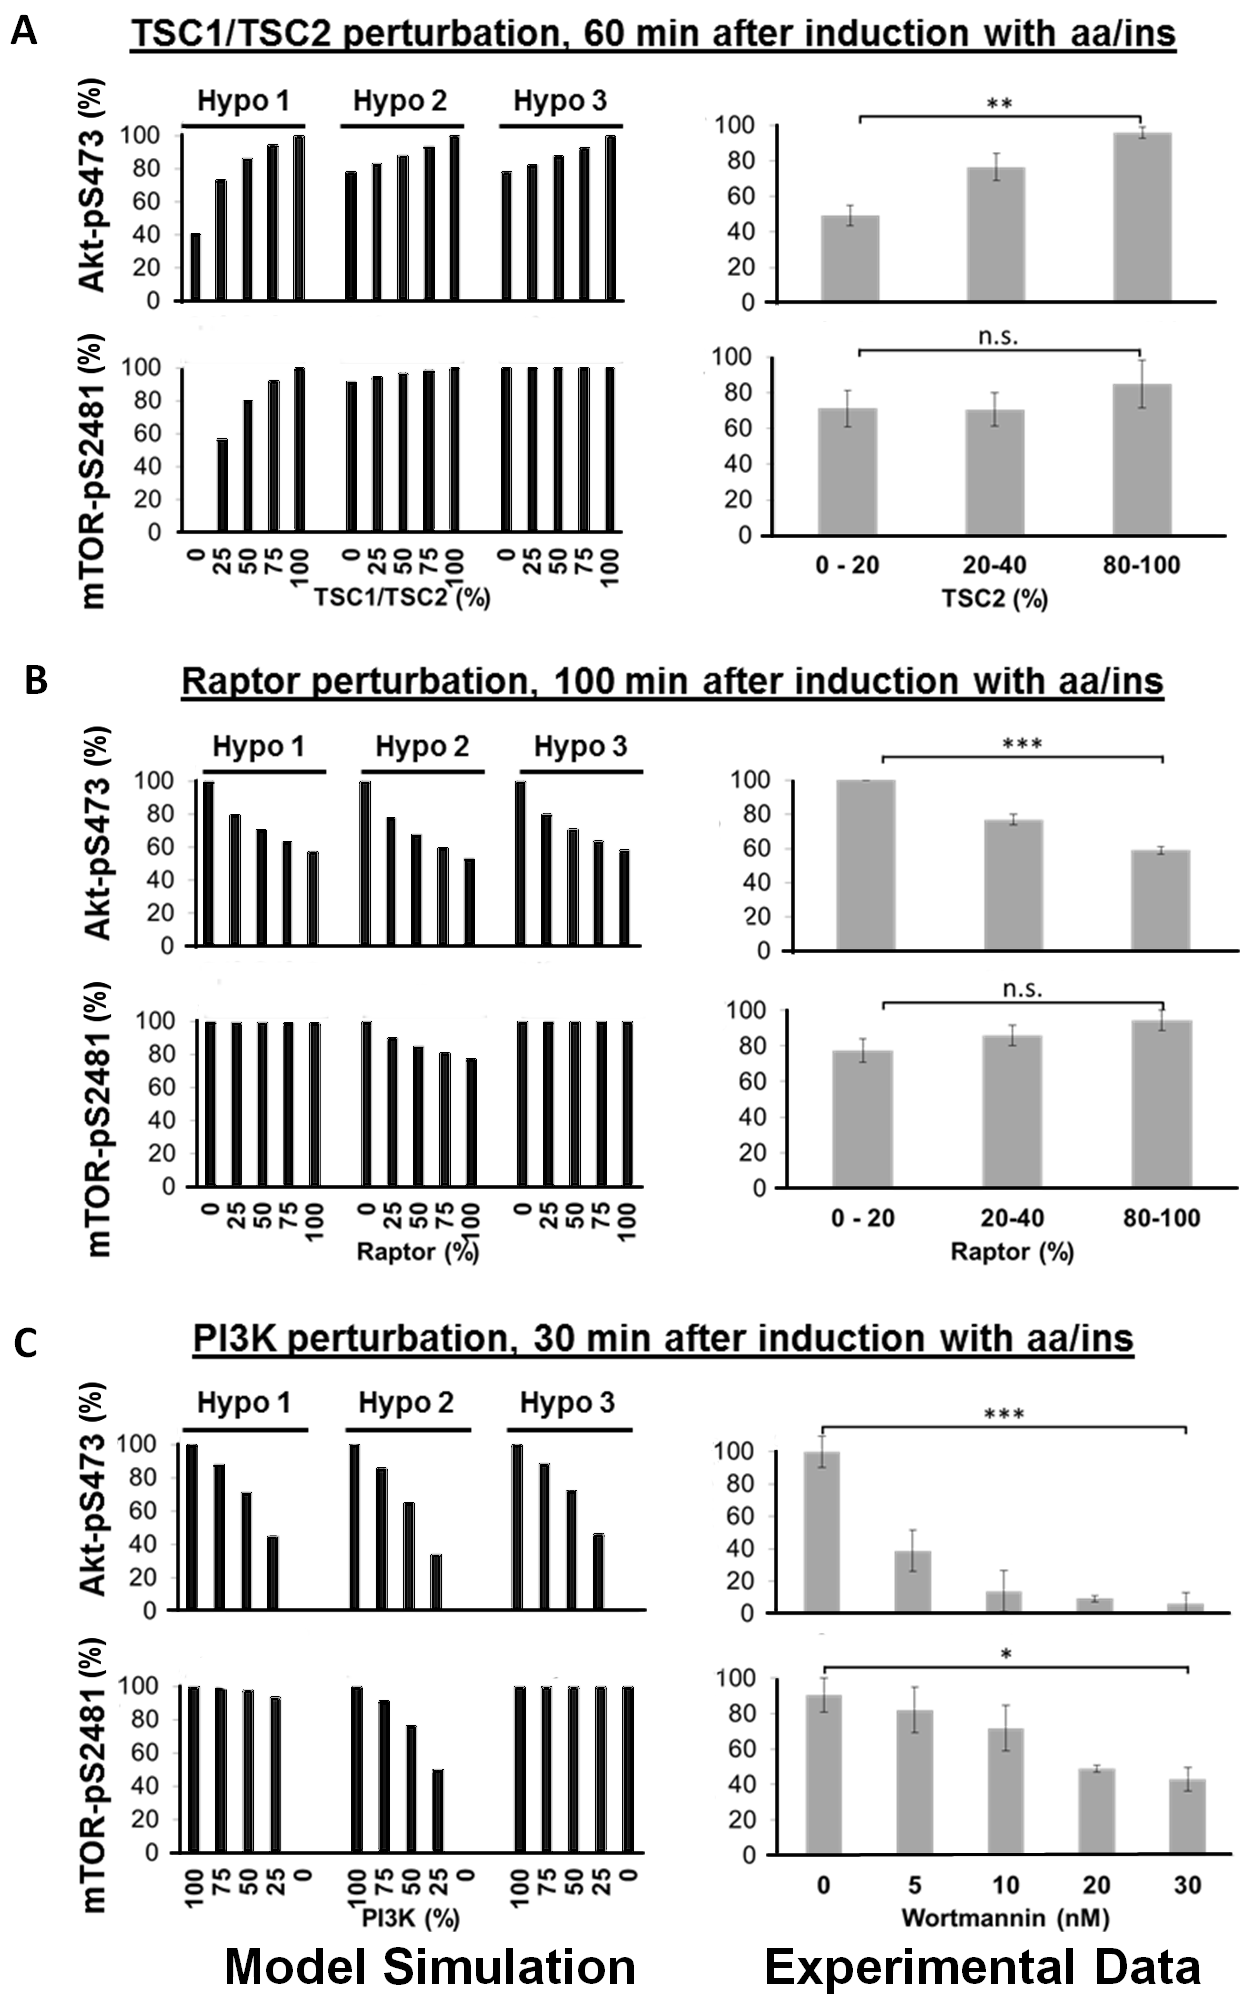
\includegraphics[width=4.0in]{2002469_fig678.png}
		%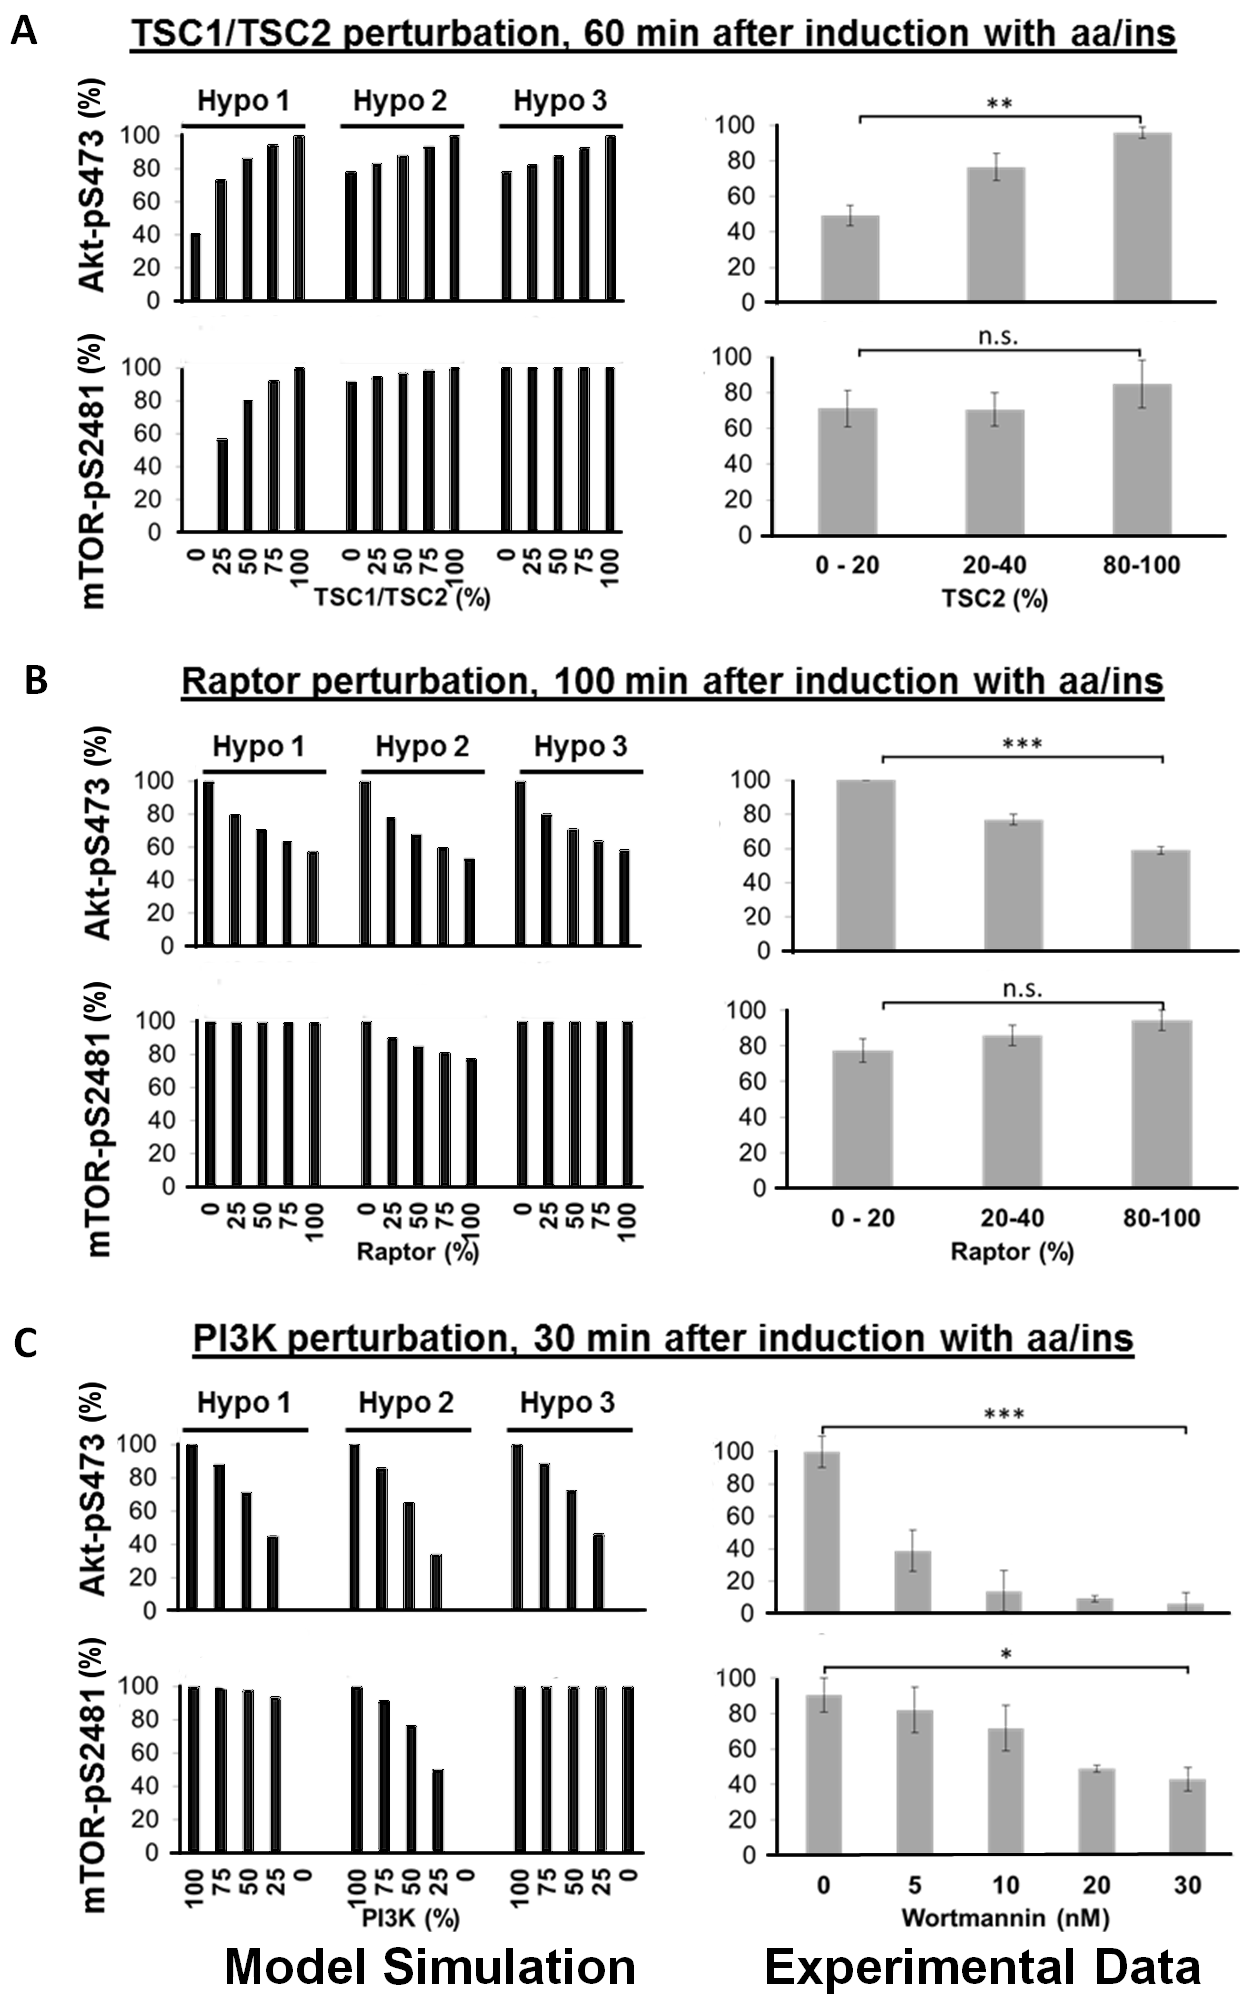
\includegraphics[scale=0.8]{2002469_fig678.png}
		\caption[Quantitative representations of simulated and experimentally determined Akt-pS473 and mTOR-pS2481]{Quantitative representations of simulated and experimentally determined Akt-pS473 and mTOR-pS2481. 
		(A) mTOR-pS2481 is not affected in response to a gradual TSC2 knock down for 60 min after induction with amino acids/insulin. 
		(B) mTOR-pS2481 is not affected by the NFL in response to Raptor knock down for 100 min after induction with amino acids/insulin. 
		(C) mTOR-pS2481 is sensitive to the PI3K inhibitor Wortmannin (Wmn) for 30 min after induction with amino acids/insulin. Data are the average and SEM computed from 3 repeats. * $P\;<\;0.05$, ** $P\;<\;0.01$, *** $P\;<\;0.001$, n.s. not significant. d = days, Hypo = hypothesis. \emph{In vitro} experiments were performed by Annika Sonntag, Freiburg University, Germany.}
		\label{fig:2002469_fig678}
	\end{center}
\end{figure}
\clearpage

\begin{figure}[tb]
	\begin{center}
		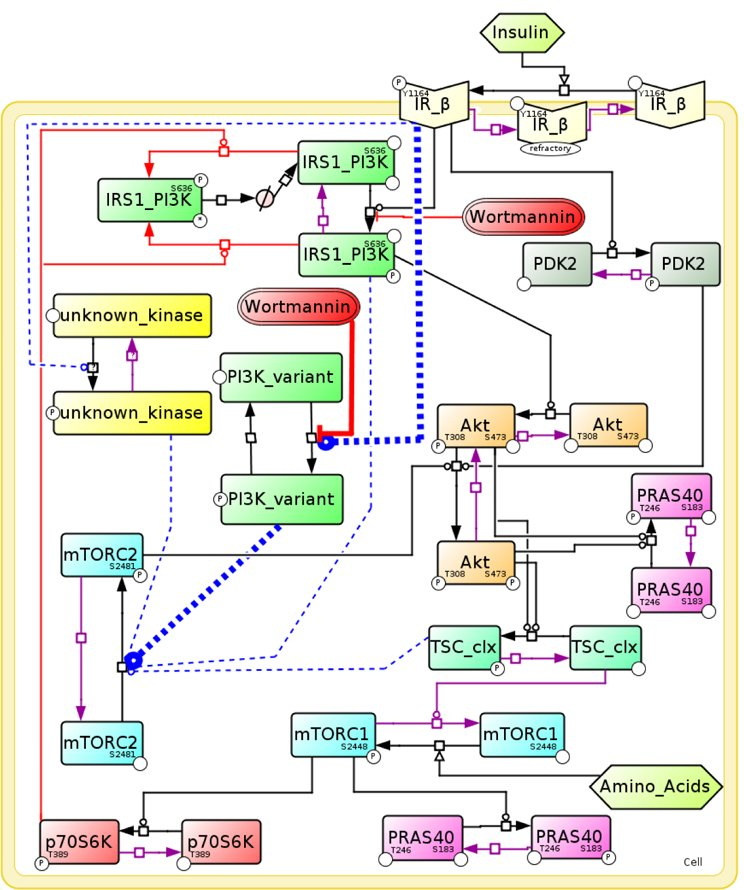
\includegraphics[scale=1.8]{2002469_fig9B.jpg}
		\caption[A new hypothesis and network structure for mTORC2 regulation by insulin]{A new hypothesis and network structure for mTORC2 regulation by insulin. Schematic representation of the pathway for Hypothesis 4: Insulin induction of mTORC2 by a PI3K (red) that is insensitive to TSC1/TSC2 and to the S6K to IRS-mediated NFL. This hypothesis was equivalent to Hypothesis 3 (PI3K and TSC1/TSC2-independent activation), assuming that the mTORC2 activator was sensitive to Wortmannin.}
		\label{fig:2002469_fig9B}
	\end{center}
\end{figure}

\clearpage
\begin{figure}[tb]
	\begin{center}
		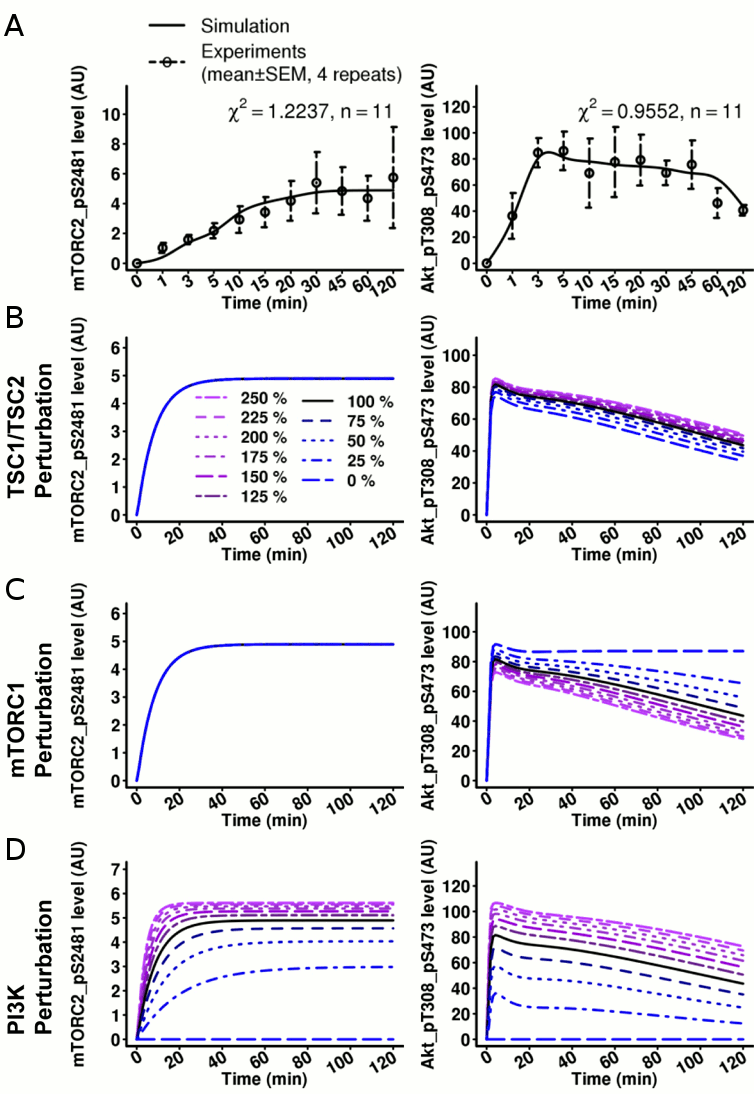
\includegraphics[scale=1.35]{2002469_fig9CF.png}
		\caption[A new hypothesis and network structure for mTORC2 regulation by insulin]{A new hypothesis and network structure for mTORC2 regulation by insulin. (A) The model simulation data for Hypothesis match the experimental dynamical phosphorylation data. The simulated and experimentally measured dynamics are shown for the mTORC2 readouts mTOR-pS2481 and Akt-pS473 (see Figure \ref{fig:2002469_supp_fig16} for all other readouts). (B) Predictions for mTOR-pS2481 and Akt-pS473 upon gradual TSC1/TSC2 knock down match the experimental data, which is presented in Figure \ref{fig:2002469_fig678}A. Whereas at 60 min after induction Akt-pS473 is gradually reduced by TSC2 inhibition, mTOR-pS2481 is TSC2-insensitive. See Figure \ref{fig:2002469_supp_fig16} for Akt-pT308 and p70-S6K-pT389. (C) Predictions for mTOR-pS2481 and Akt-pS473 readouts upon gradual Raptor knock down match the experimental data, which is presented in Figure \ref{fig:2002469_fig678}B. Whereas at 100 min after induction Akt-pS473 is gradually 
induced by Raptor inhibition, mTOR-pS2481 is Raptor-insensitive. See Figure \ref{fig:2002469_supp_fig16} for Akt-pT308 and p70-S6K-pT389. (D) Predictions for mTOR-pS2481 and Akt-pS473 readouts upon gradual PI3K inhibition match the experimental data, which is presented in Figure \ref{fig:2002469_fig678}C. Both Akt-pS473 and mTOR-pS2481 are gradually reduced by Wortmannin at 30 min after induction. See Figure \ref{fig:2002469_supp_fig16} for Akt-pT308 and p70-S6K-pT389. \emph{In vitro} experiments were performed by Annika Sonntag, Freiburg University, Germany.}
		\label{fig:2002469_fig9CF}
	\end{center}
\end{figure}
\clearpage

\begin{figure}[tb]
	\begin{center}
		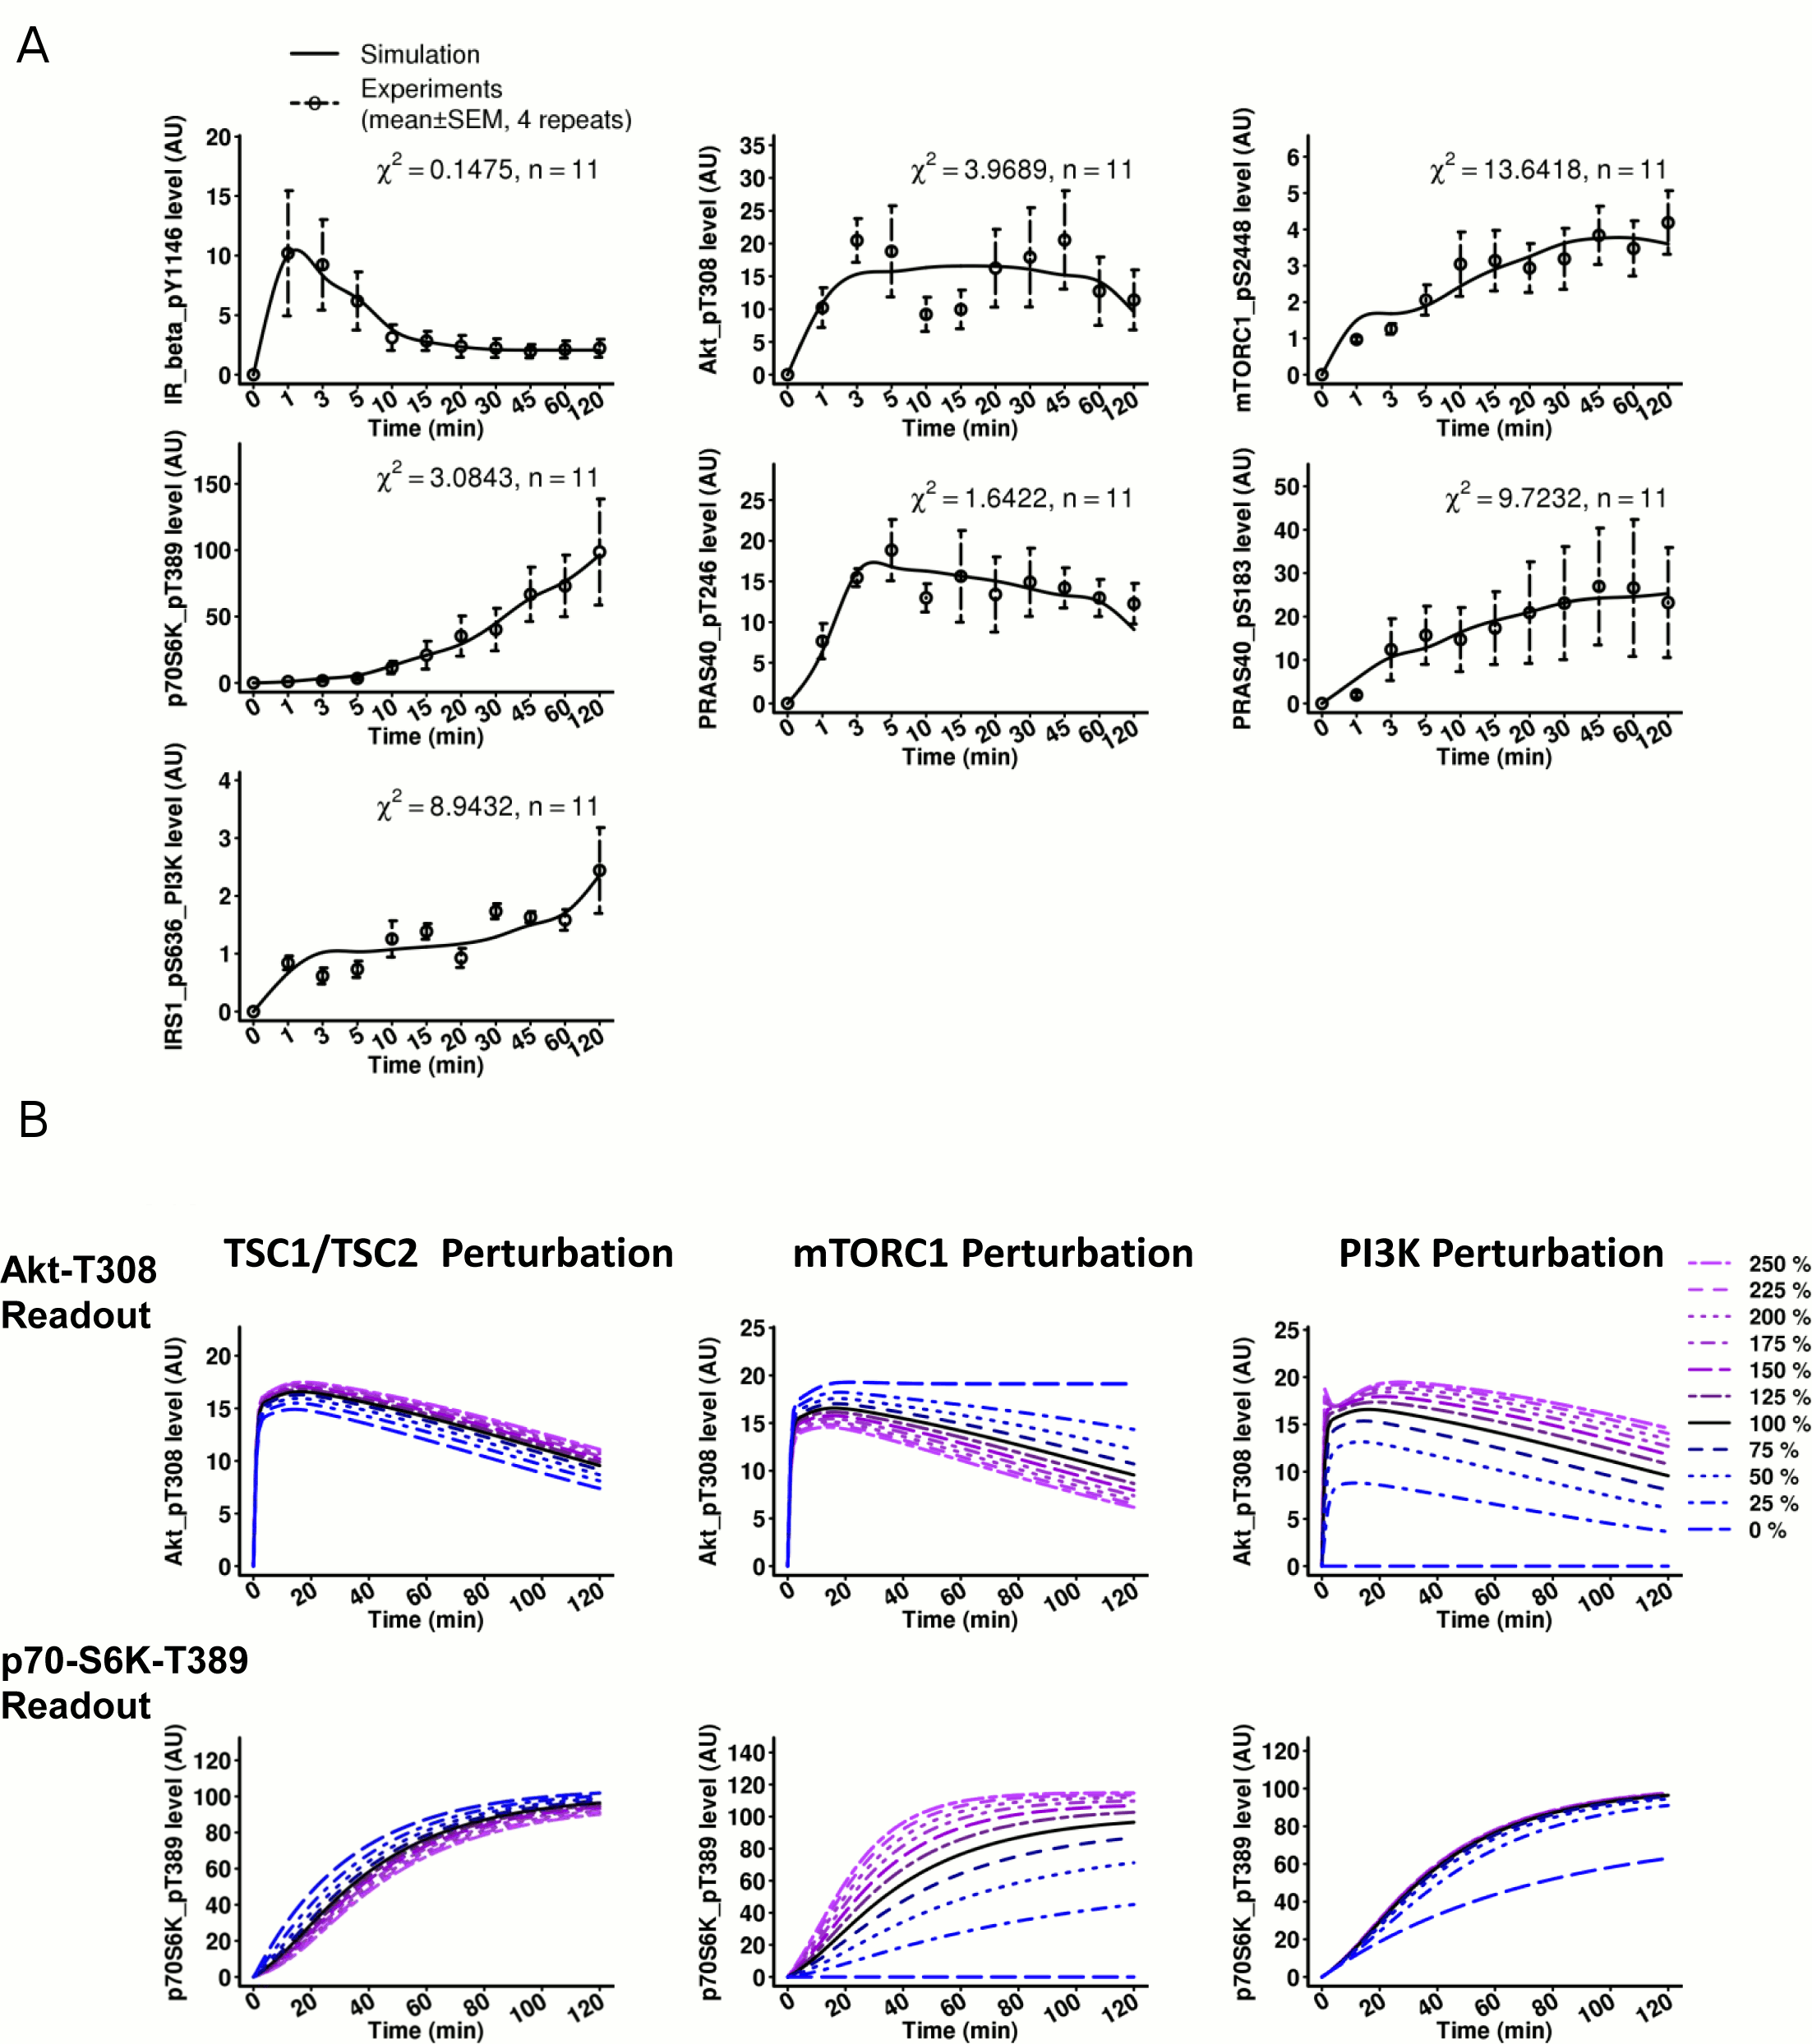
\includegraphics[scale=0.75]{2002469_supp_fig16.png}
		\caption[Simulation and perturbations for the new network structure based on Hypothesis 4: PI3K-dependent, NFL-independent regulation of mTORC2]{Simulation and perturbations for the new network structure based on Hypothesis 4: PI3K-dependent, NFL-independent regulation of mTORC2. (A) Comparison between the simulated and experimental time courses for Hypothesis 4 shows that the simulated time courses match the experimental readouts. (B) The influence of perturbations of TSC1/TSC2, mTORC1, or PI3K on the dynamics of phosphorylation of Akt-T308 and p70-S6K-T389 for Hypothesis 4. \emph{In vitro} experiments were performed by Annika Sonntag, Freiburg University, Germany.}
		\label{fig:2002469_supp_fig16}
	\end{center}
\end{figure}
\clearpage

\begin{figure}[tb]
	\begin{center}
		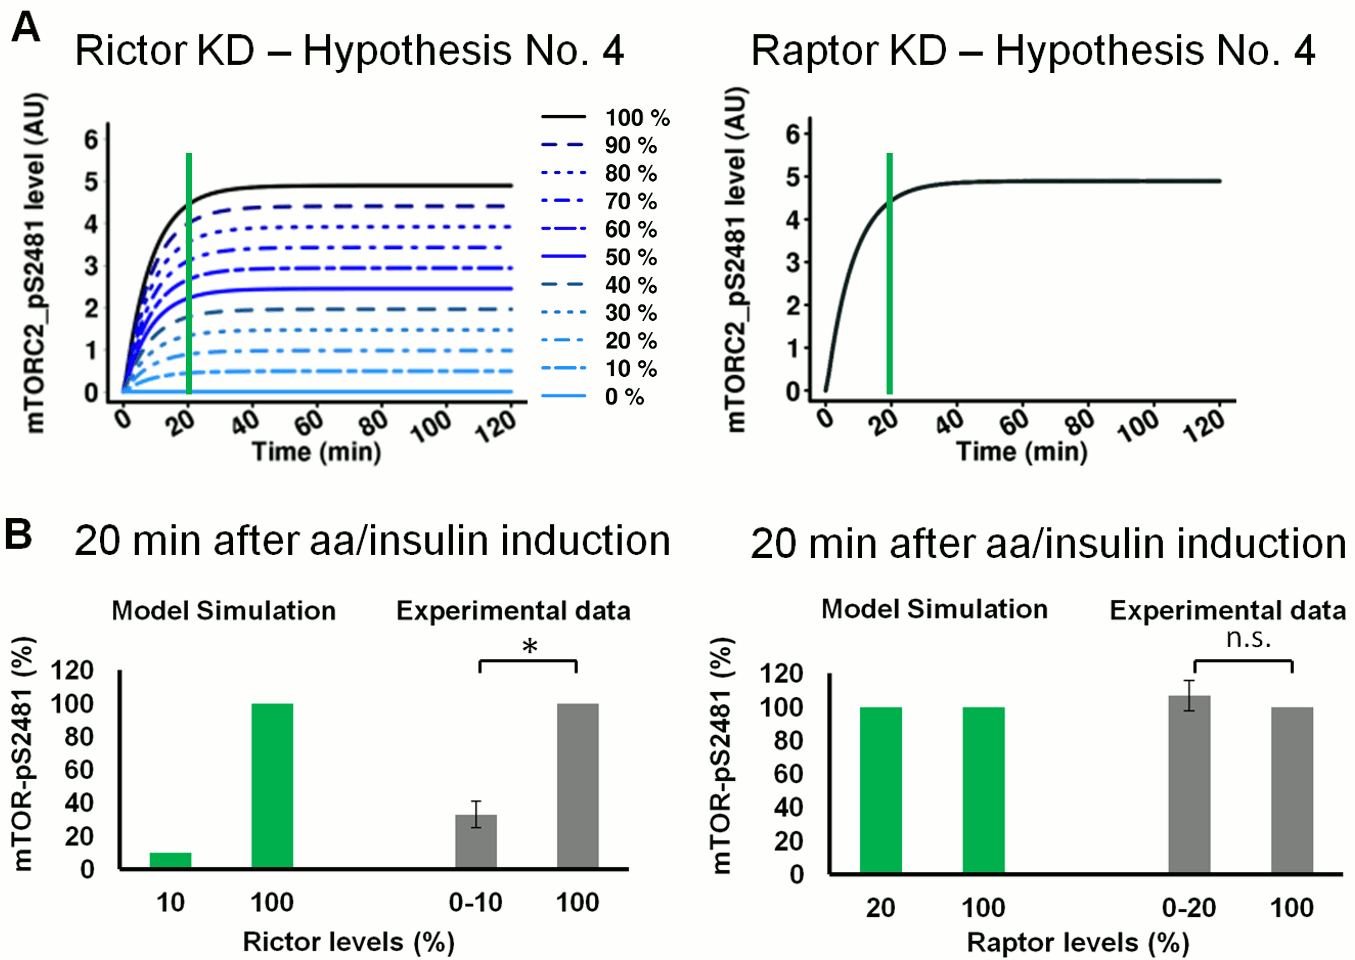
\includegraphics[scale=1]{response_letter_fig1.png}
		\caption[Validation Hypothesis 4 by Rictor and Raptor knock down.]{Validation Hypothesis 4 by Rictor and Raptor knock down. (A) Simulation of mTOR-pS2481 dynamic in response to addition of amino acids and insulin when Rictor or Raptor is knocked down (KD). (B) Quantifications of the simulations and experimental data for mTOR-pS2481 upon Rictor or Raptor knock down 20 min after amino acids/insulin induction. * $P\;<\;0.01$; n.s., not significant; Student's $t$-test. \emph{In vitro} experiments were performed by Annika Sonntag, Freiburg University, Germany. (See \citep[Fig. 1]{DallePezze2012b}).}
		\label{fig:response_letter_fig1}
	\end{center}
\end{figure}
\clearpage

\begin{figure}[tb]
	\begin{center}
		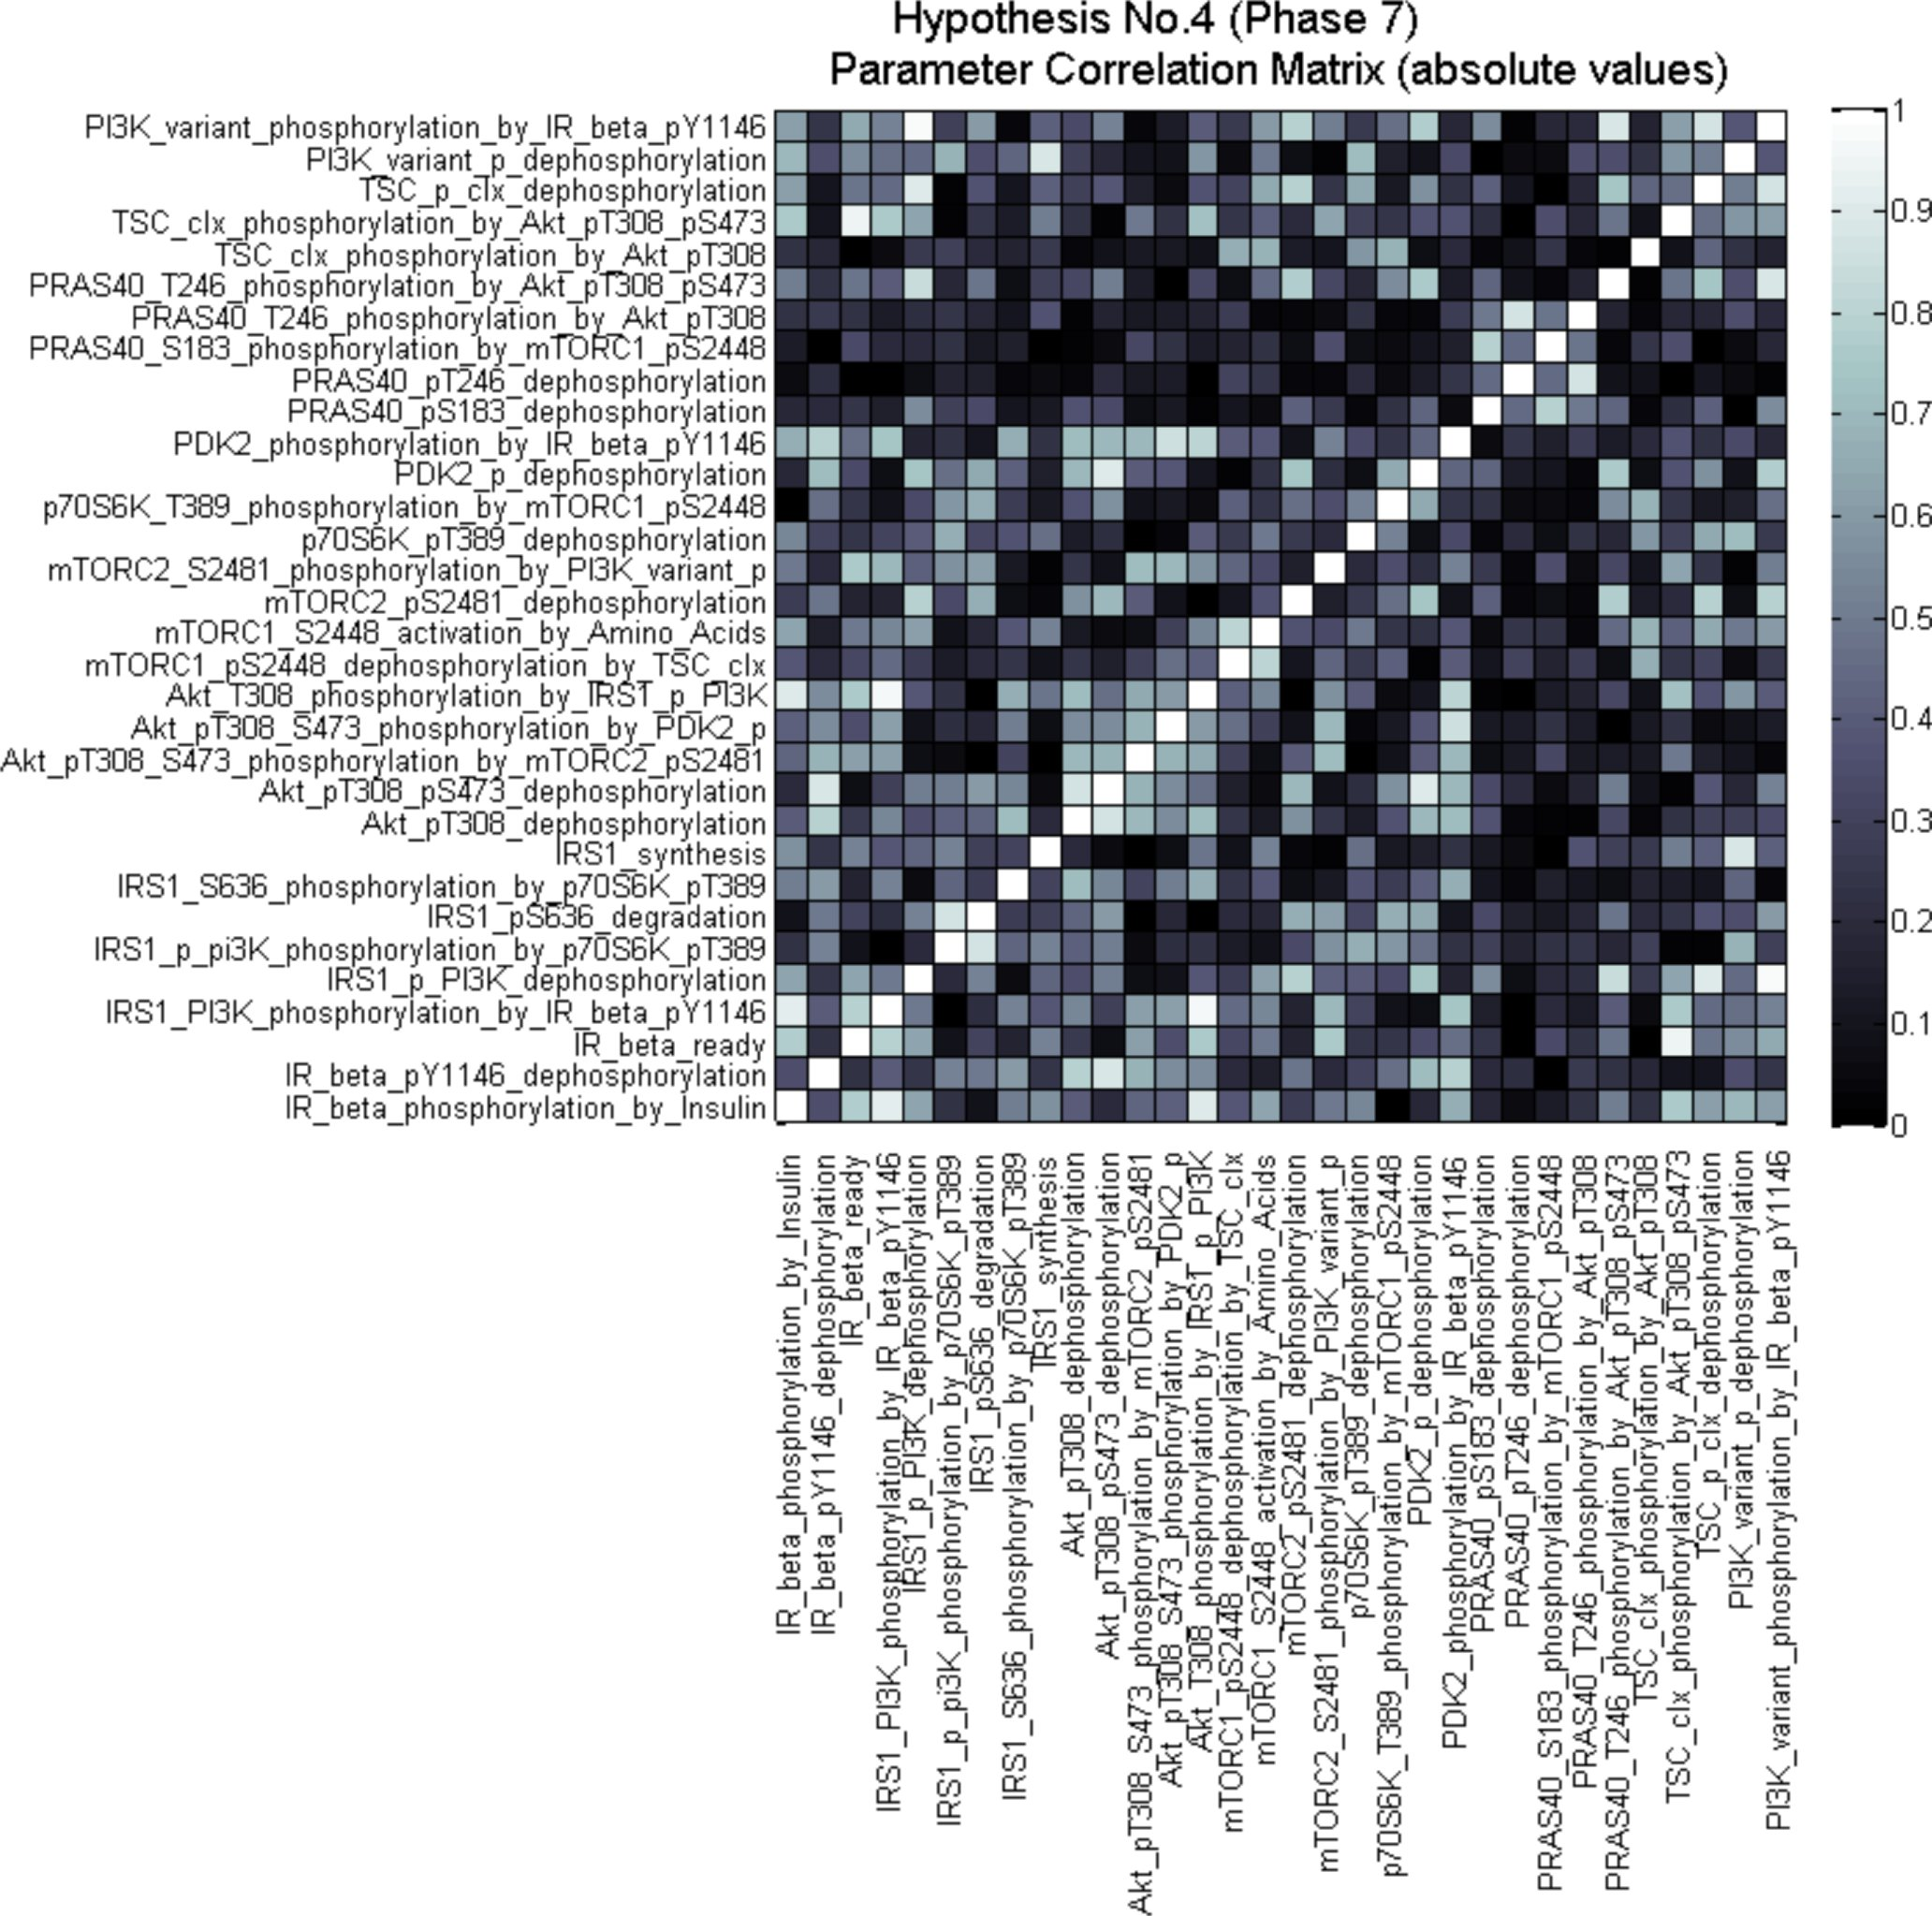
\includegraphics[scale=0.8]{2002469_supp_fig17.jpg}
		\caption[Identifiability analysis for Hypothesis 4: PI3K-dependent, NFL-independent regulation of mTORC2]{Identifiability analysis for Hypothesis 4: PI3K-dependent, NFL-independent regulation of mTORC2. Parameter correlation matrix for Hypothesis 4 is shown. See Figure \ref{fig:2002469_supp_fig5} for details.}
		\label{fig:2002469_supp_fig17}
	\end{center}
\end{figure}
\clearpage

\begin{figure}[tb]
	\begin{center}
		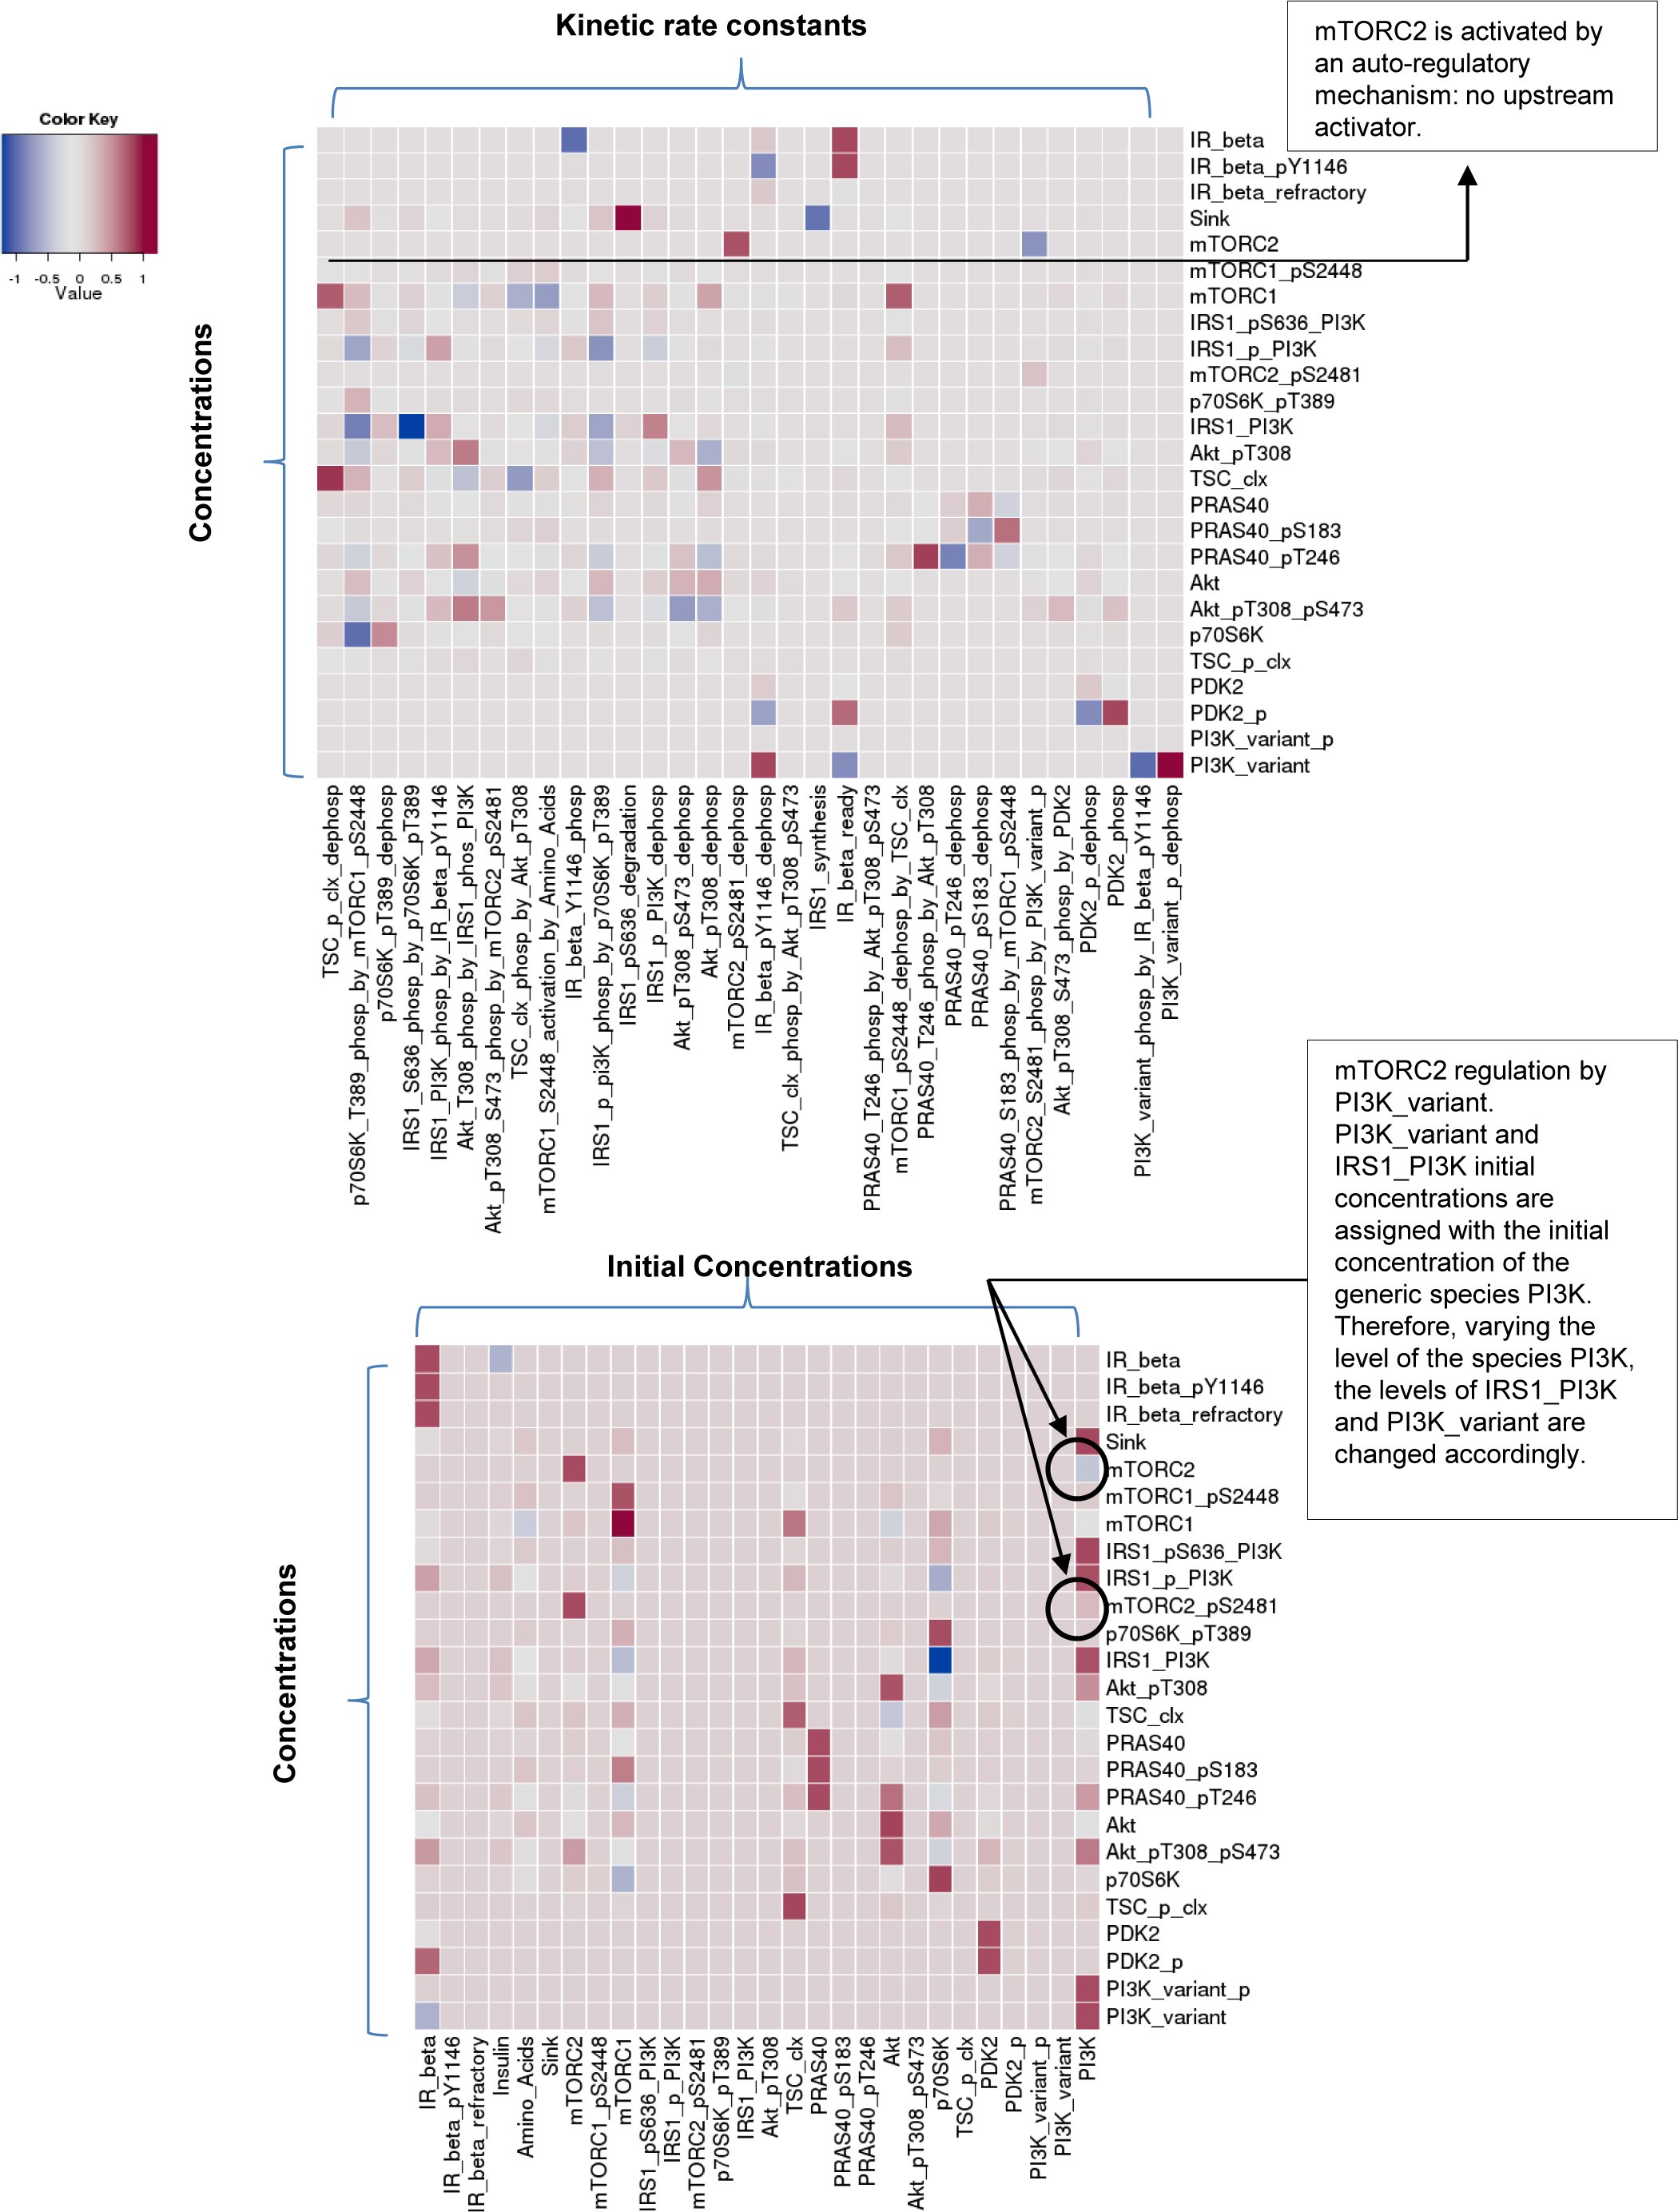
\includegraphics[scale=0.75]{2002469_supp_fig18.jpg}
		\caption[Sensitivity analysis for Hypothesis 4: PI3K-dependent, NFL-independent regulation of mTORC2]{Sensitivity analysis for Hypothesis 4: PI3K-dependent, NFL-independent regulation of mTORC2. Sensitivity analysis for the initial concentrations and the kinetic rates parameters for Hypothesis 4 is shown. See Figure \ref{fig:2002469_supp_fig6} for details of the top and bottom plots.}
		\label{fig:2002469_supp_fig18}
	\end{center}
\end{figure}
\clearpage






%\section{Tables}
%\label{paper1-sec:Tables}

\begin{table}[tb]
	\begin{center}
		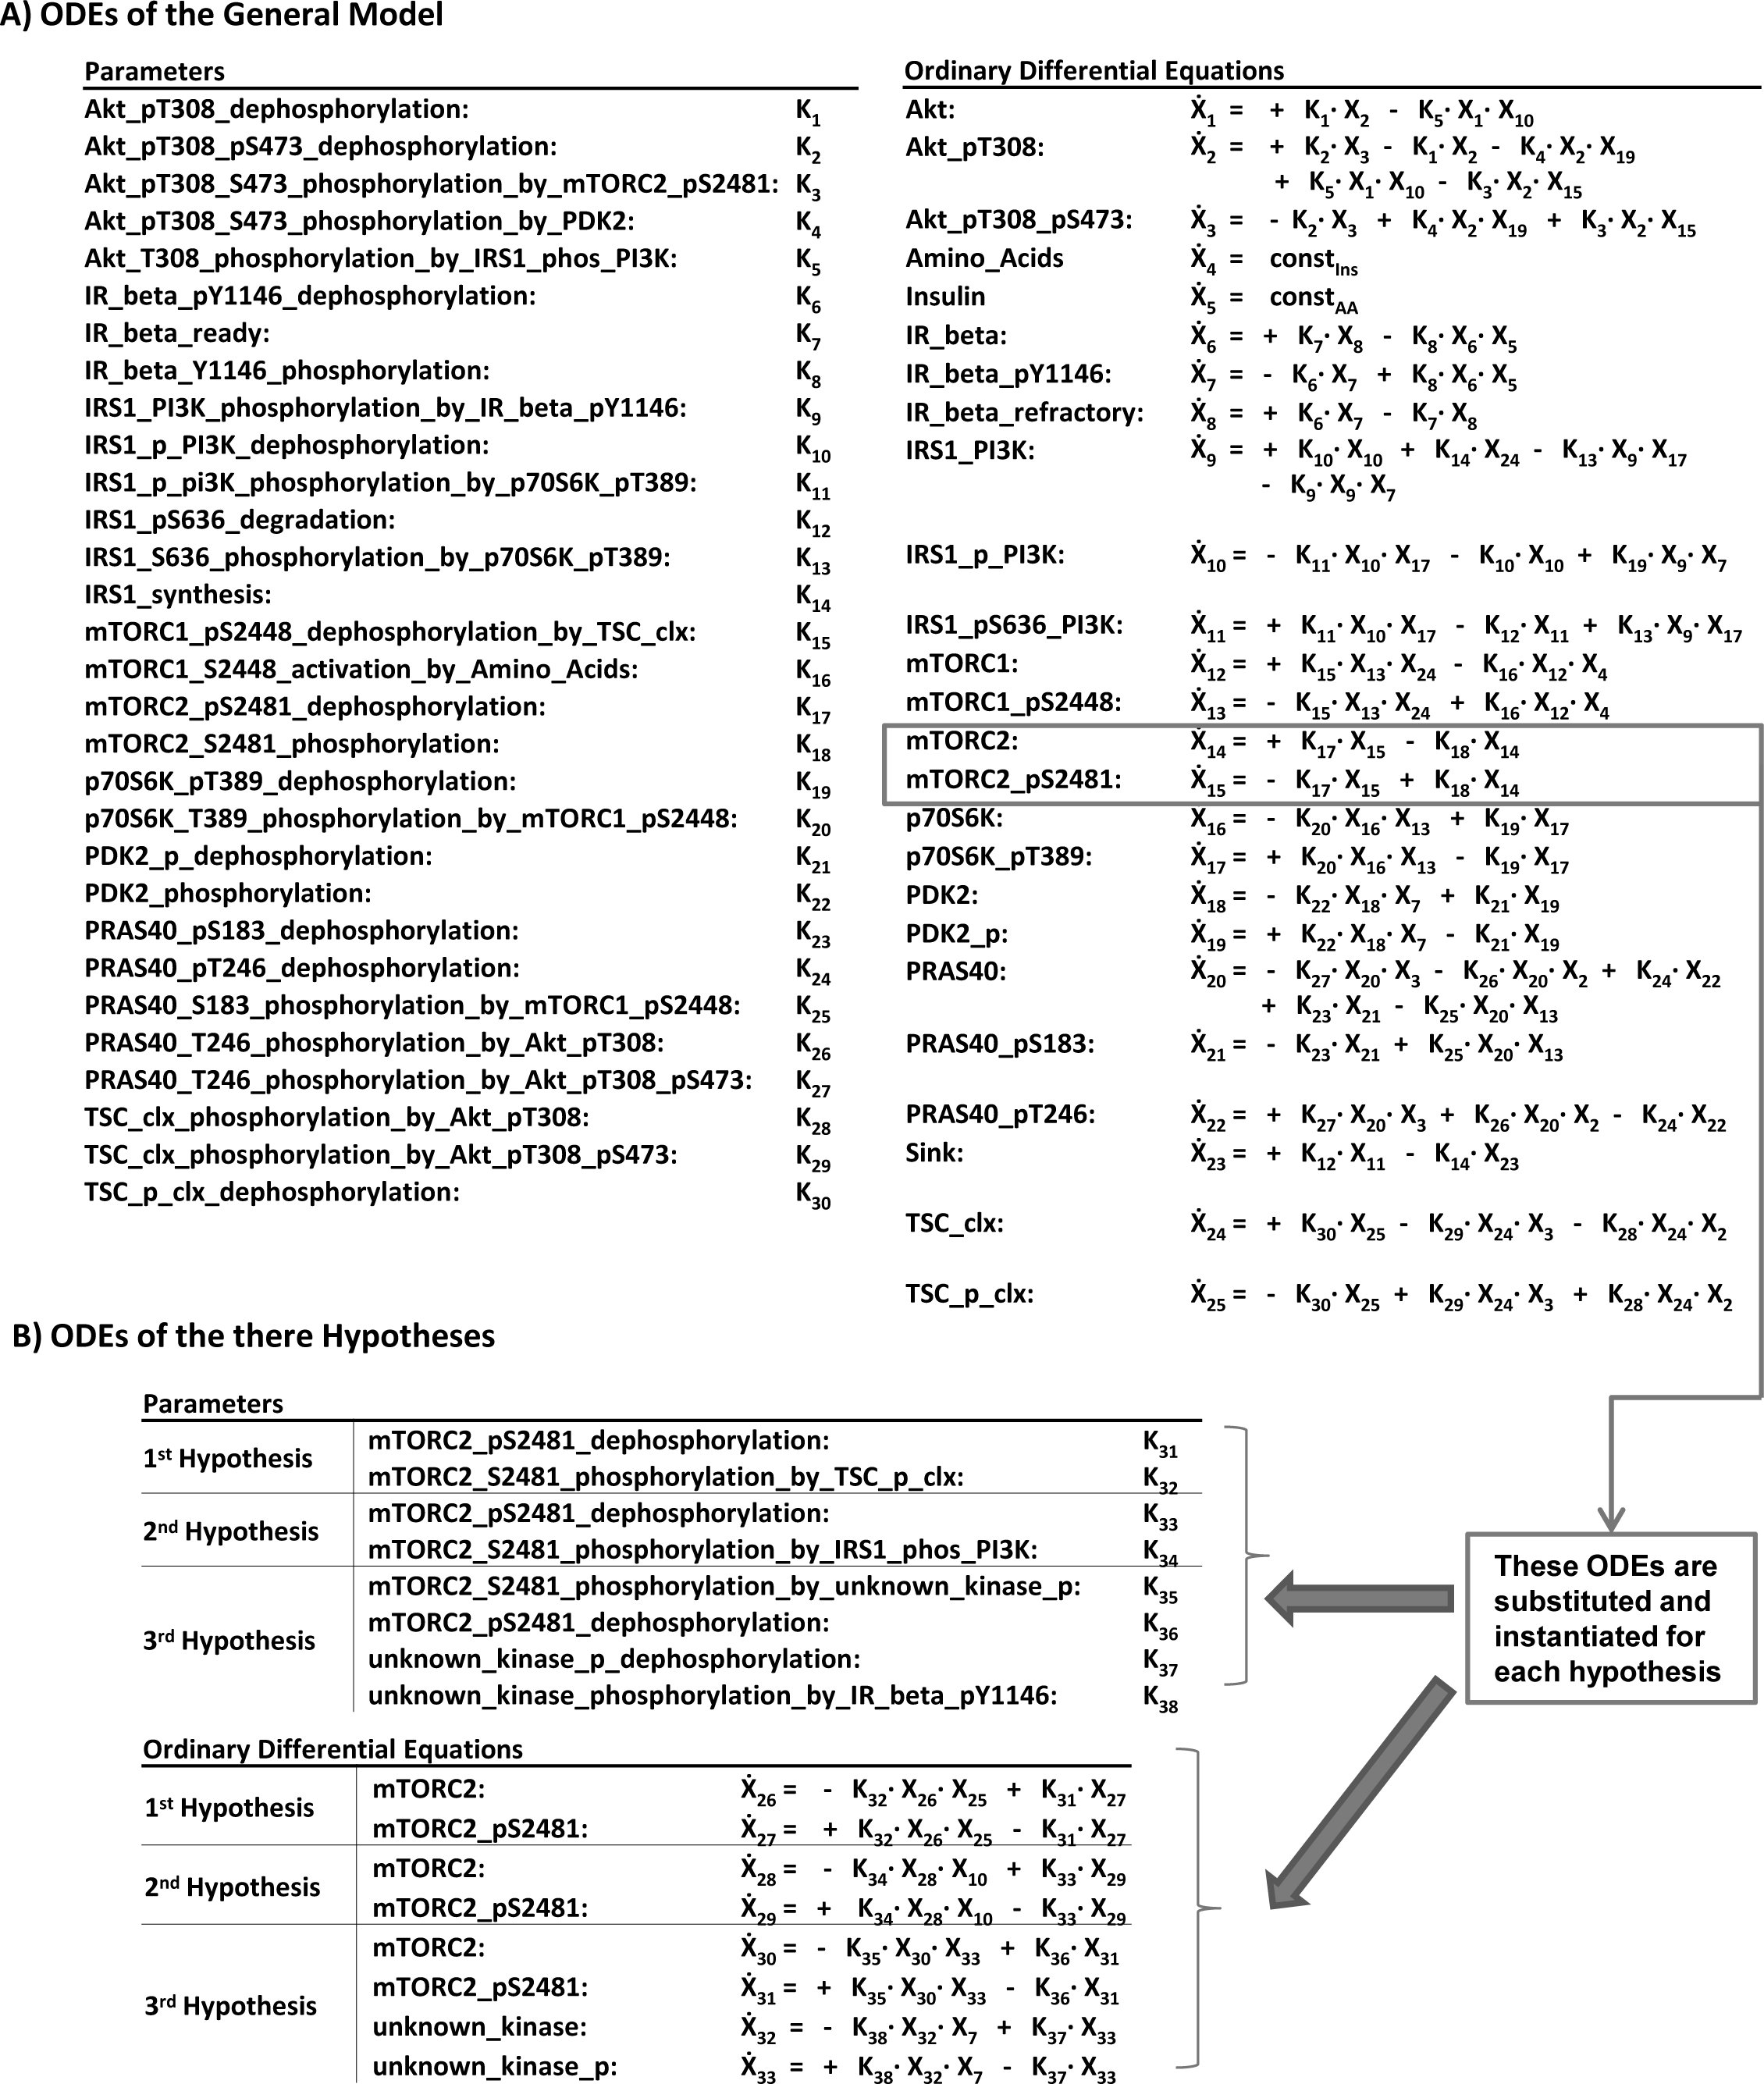
\includegraphics[scale=0.75]{2002469_supp_tab1.png}
		\caption[Ordinary differential equations of the general model and the models representing Hypothesis 1, 2, and 3 for mTORC2 activation]{Ordinary differential equations of the general model and the models representing Hypothesis 1, 2, and 3 for mTORC2 activation. List of kinetic rate constants and ordinary differential equations (ODEs) for the general model (A) and the Hypotheses 1, 2, and 3 (B). Each hypothesis is derived from the general model by replacing the mTORC2 ODEs, shown in the box, with those corresponding to the hypothesis.}
		\label{tab:2002469_supp_tab1}
	\end{center}
\end{table}
\clearpage

\begin{table}[tb]
	\begin{center}
		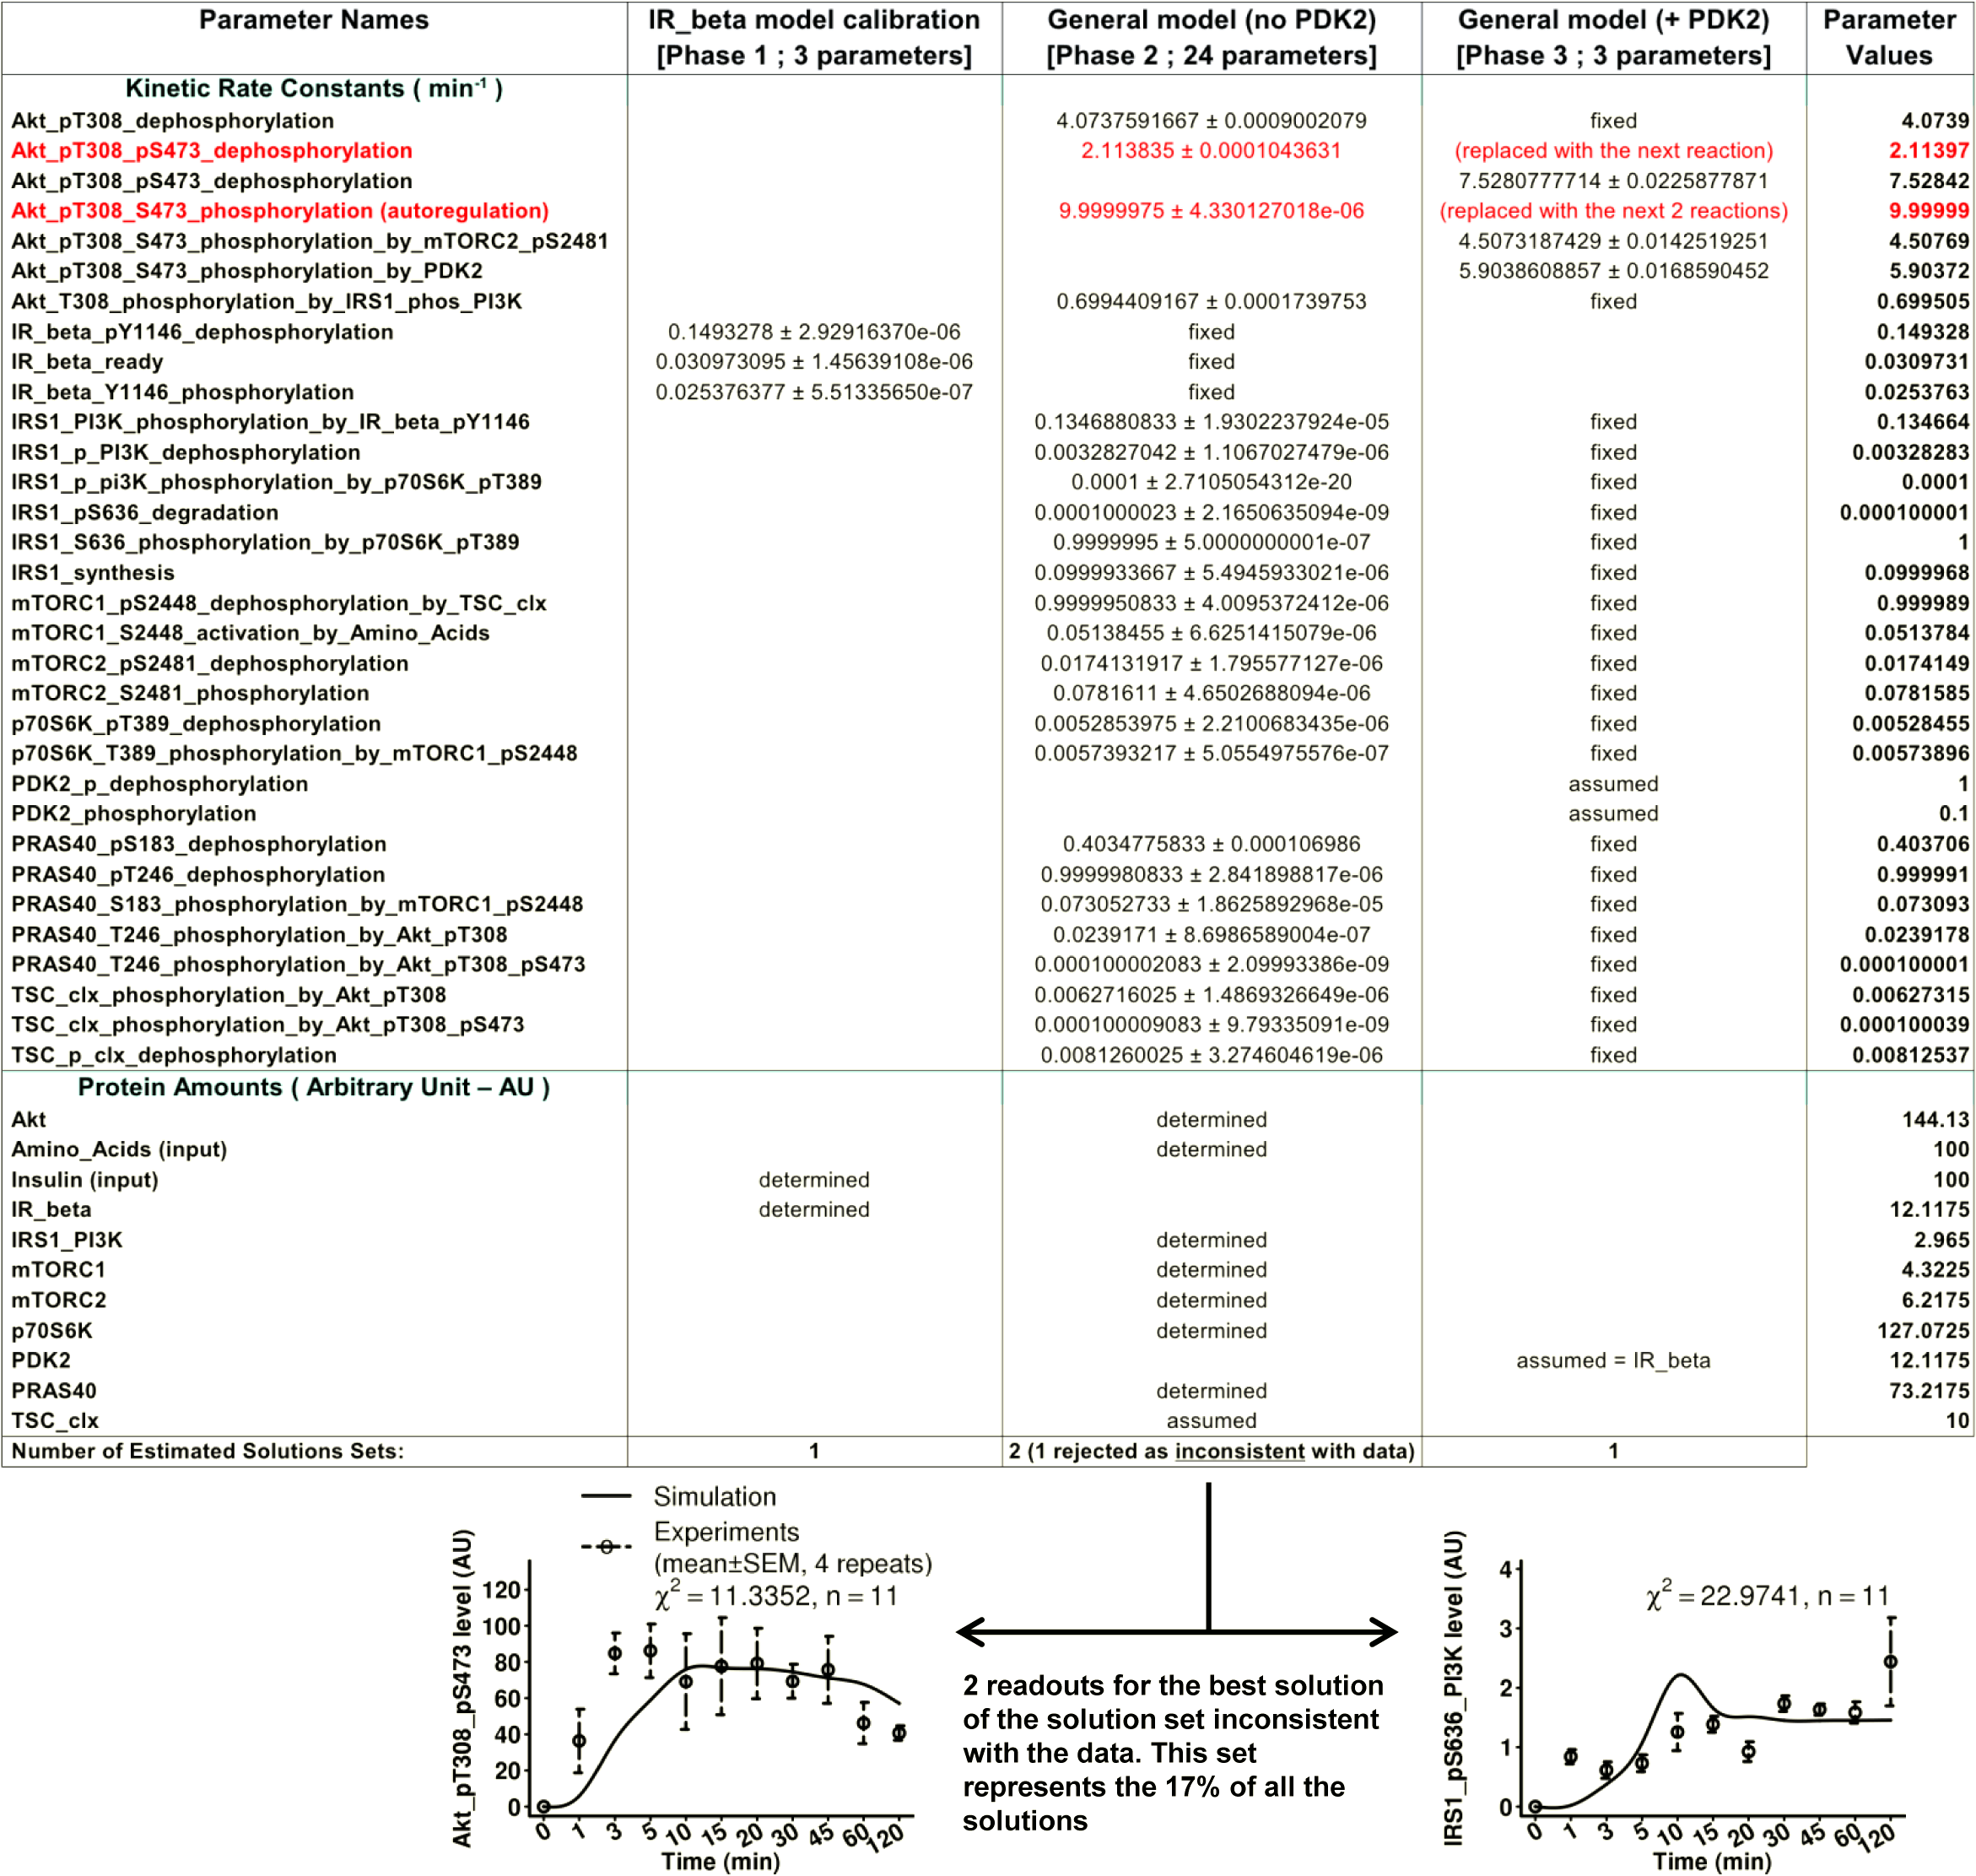
\includegraphics[scale=0.72]{2002469_supp_tab2.png}
		\caption[Parameter values of the general model]{Parameter values of the general model. The general model was fully parameterised by three steps. Phase 1, 3 kinetic rate constants of the insulin receptor (IR-beta) were determined. Phase 2, the general model without PDK2 was obtained by parameterising 24 kinetic rate constants. In this phase, Akt-S473 activation is modelled as autoregulation, independent of mTORC2 and PDK2. Phase 3, PDK2 dynamics were added to the system and the 3 parameters regulating Akt-S473 phosphorylation were calibrated by substituting the previously introduced autoregulatory mechanism (parameters values shown in red) of Akt. For each phase, 350 independent calibrations, starting from random initial configurations of the parameters, were executed and the best solution set fitting the data was selected. Phase 1 and 3 converged to a single solution set. Phase 2 converged to two solutions sets of which one was discarded as inconsistent with the experimental data (shown for phosphorylated 
Akt-S473 and IRS1-S636 readouts). For each phase, the mean and standard deviation of the estimated parameters were computed from the selected solution set. The solution closest to the centroid of the selected solution cluster was chosen for fixing the parameter values. \emph{In vitro} experiments were performed by Annika Sonntag, Freiburg University, Germany.}
		\label{tab:2002469_supp_tab2}
	\end{center}
\end{table}
\clearpage

\begin{table}[tb]
	\begin{center}
		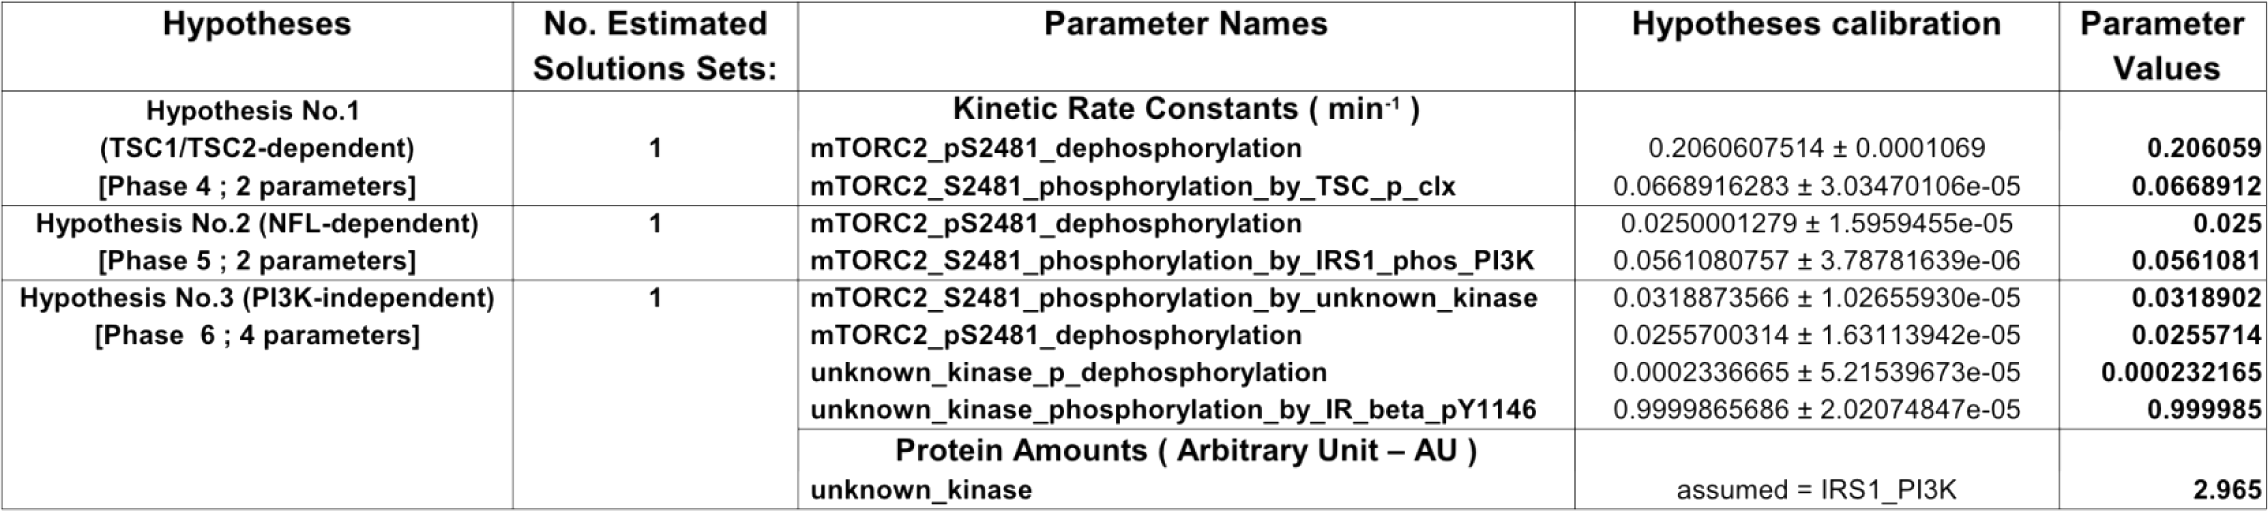
\includegraphics[scale=0.75]{2002469_supp_tab3.png}
		\caption[Parameter values of Hypotheses 1, 2, and 3]{Parameter values of Hypotheses 1, 2, and 3. For each hypothesis, the estimated parameters were calibrated using the same protocol provided in Table \ref{tab:2002469_supp_tab2}. For each hypothesis, all the corresponding calibrations converged to a single solution set.}
		\label{tab:2002469_supp_tab3}
	\end{center}
\end{table}
\clearpage

\begin{table}[tb]
	\begin{center}
		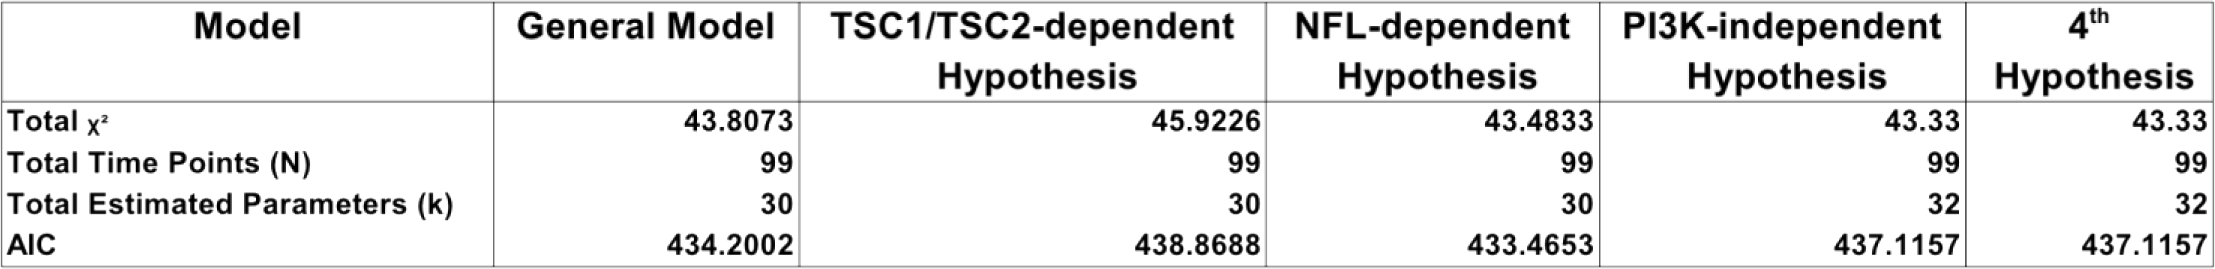
\includegraphics[scale=0.75]{2002469_supp_tab4.png}
		\caption[Summary of model goodness-of-fit]{Summary of model goodness-of-fit. The total $\chi^2$ and Akaike Information Criterion (AIC) measures are reported for the general model and the four hypotheses. Both the measures slightly penalise the TSC1/TSC2-dependent hypothesis. AIC also penalises the PI3K-independent and the fourth hypotheses due to the higher number of parameters in these two models. However, these differences are not statistically significant for rejection of any model.}
		\label{tab:2002469_supp_tab4}
	\end{center}
\end{table}
\clearpage




% ------------------------------------------------------------------------

%%% Local Variables: 
%%% mode: latex
%%% TeX-master: "../thesis"
%%% End: 
